% ---------------------------------------------------------------------------
% ---------------------------------------------------------------------------
% Modelo LaTex para preparação do documento final de Monografia TCC
% O modelo está em conformidade com ABNT NBR
% ---------------------------------------------------------------------------
% ---------------------------------------------------------------------------
\newcommand\myworries[1]{\textcolor{red}{#1}}

\documentclass[
	% -- opções da classe memoir --
	12pt,					% tamanho da fonte
	openright,				% capítulos começam em pág ímpar (insere página vazia caso preciso)
	oneside,					% para impressão em verso e anverso. Oposto a oneside
	a4paper,					% tamanho do papel. 
	% -- opções da classe abntex2 --
	%chapter=TITLE,			% títulos de capítulos convertidos em letras maiúsculas
	%section=TITLE,			% títulos de seções convertidos em letras maiúsculas
	%subsection=TITLE,		% títulos de subseções convertidos em letras maiúsculas
	%subsubsection=TITLE,	% títulos de subsubseções convertidos em letras maiúsculas
	% -- opções do pacote babel --
	english,					% idioma adicional para hifenização
	%french,					% idioma adicional para hifenização
	%spanish,				% idioma adicional para hifenização
	brazil					% o último idioma é o principal do documento
	]{abntex2}

% ---------------------
% Pacotes OBRIGATÓRIOS
% ---------------------
\usepackage{lmodern}				% Usa a fonte Latin Modern			
\usepackage[T1]{fontenc}			% Selecao de codigos de fonte.
\usepackage[utf8]{inputenc}		% Codificacao do documento (conversão automática dos acentos)
\usepackage{lastpage}			% Usado pela Ficha catalográfica
\usepackage{indentfirst}			% Indenta o primeiro parágrafo de cada seção.
\usepackage{color}				% Controle das cores
\usepackage{graphicx,graphicx}	% Inclusão de gráficos
\usepackage{epsfig,subfig}		% Inclusão de figuras
\usepackage{float}              %delimitar posição de figura
\usepackage{microtype} 			% Melhorias de justificação
% ---------------------
		
% ---------------------
% Pacotes ADICIONAIS
% ---------------------
\usepackage{lipsum}						% Geração de dummy text
\usepackage{amsmath,amssymb,mathrsfs}	% Comandos matemáticos avançados 
\usepackage{setspace}  					% Para permitir espaçamento simples, 1 1/2 e duplo
\usepackage{verbatim}					% Para poder usar o ambiente "comment"
\usepackage{tabularx} 					% Para poder ter tabelas com colunas de largura auto-ajustável
\usepackage{afterpage} 					% Para executar um comando depois do fim da página corrente
\usepackage{url} 	% Para formatar URLs (endereços da Web)
% ---------------------

\usepackage{svg}    %usar arquivo.svg

% ---------------------
% Pacotes de CITAÇÕES
% ---------------------
\usepackage[brazilian,hyperpageref]{backref}	% Paginas com as citações na bibl
\usepackage[alf]{abntex2cite}				% Citações padrão ABNT (alfa)
%\usepackage[num]{abntex2cite}				% Citações padrão ABNT (numericas)
% ---------------------

% Configurações de CITAÇÕES para abntex2
% --- 
% CONFIGURAÇÕES DE PACOTES
% --- 

% ---
% Configurações do pacote backref
% Usado sem a opção hyperpageref de backref
\renewcommand{\backrefpagesname}{Citado na(s) página(s):~}
% Texto padrão antes do número das páginas
\renewcommand{\backref}{}
% Define os textos da citação
\renewcommand*{\backrefalt}[4]{
	\ifcase #1 %
		Nenhuma citação no texto.%
	\or
		Citado na página #2.%
	\else
		Citado #1 vezes nas páginas #2.%
	\fi}%
% ---

% Inclusão de dados para CAPA e FOLHA DE ROSTO (título, autor, orientador, etc.)
% ---
% Informações de dados para CAPA e FOLHA DE ROSTO
% ---
\titulo{Controle e Automação de Vant com Visão Computacional para Sensoriamento Populacional}
\autor{Fabiano Dutra Filereno}
\local{Porto Alegre-RS}
\data{2020}
\orientador{prof. Dr. Leonardo Albernaz Amaral}
%\coorientador{Fulano Coorientador}
\instituicao{%
  Centro Universitário Uniftec}
\tipotrabalho{Trabalho de Conclusão de Curso (TCC)}
% O preambulo deve conter o tipo do trabalho, o objetivo,
% o nome da instituição e a área de concentração
\preambulo{Trabalho apresentado para o Curso de Engenharia do Computação, de Centro Universitário Uniftec como parte dos requisitos para avaliação da unidade curricular de TCC.}
% ---

% Inclui Configurações de aparência do PDF Final
%  Configurações de aparência do PDF final
% NÃO ALTERAR!!!

% alterando o aspecto da cor azul
\definecolor{blue}{RGB}{41,5,195}

% informações do PDF
\makeatletter
\hypersetup{
     	%pagebackref=true,
		pdftitle={\@title}, 
		pdfauthor={\@author},
    		pdfsubject={\imprimirpreambulo},
	    pdfcreator={LaTeX with abnTeX2},
		pdfkeywords={abnt}{latex}{abntex}{abntex2}{trabalho acadêmico}, 
		colorlinks=true,       		% false: boxed links; true: colored links
    		linkcolor=blue,          	% color of internal links
    		citecolor=blue,        		% color of links to bibliography
    		filecolor=magenta,      		% color of file links
		urlcolor=blue,
		bookmarksdepth=4
} 
\makeatother
% --- 

% O tamanho da identação do parágrafo é dado por:
\setlength{\parindent}{1.3cm}

% Controle do espaçamento entre um parágrafo e outro:
\setlength{\parskip}{0.2cm}  % tente também \onelineskip

% ---------------------
% Compila o indice
% ---------------------
\makeindex
% ---------------------

%%%%%%%%%%%%%%%%%%%%%%%%%%%
%%  INICIO DO DOCUMENTO  %%
%%%%%%%%%%%%%%%%%%%%%%%%%%%
\begin{document}

% Retira espaço extra obsoleto entre as frases.
\frenchspacing

% ----------------------------------------------------------
% ELEMENTOS PRÉ-TEXTUAIS (Capa, Resumo, Abstract, etc.)
% ----------------------------------------------------------
\pretextual

% Capa
% ---
% Impressão da Capa
% ---
  \begin{capa}%
    \begin{figure}[h!]%
        \centering%
        
\includegraphics[scale=0.7]{figs/logoftec1.png}%
      \end{figure}%
    \center
	\ABNTEXchapterfont\large{CURSO SUPERIOR DE ENGENHARIA DA COMPUTAÇÃO}
	%\vspace{1.5cm}

    \vfill
    \ABNTEXchapterfont\large\imprimirautor
    
    \vfill

	%\vfill
	\ABNTEXchapterfont\bfseries\LARGE\imprimirtitulo
	\vfill
%
    \large\imprimirlocal
    \linebreak
    \large\imprimirdata

    \vspace*{1cm}
  \end{capa}
% ---

% Folha de rosto (o * indica que haverá a ficha bibliográfica)
\imprimirfolhaderosto

% Imprimir Ficha Catalográfica
%% ---
% Ficha Catalográfica
% ---
% Isto é um exemplo de Ficha Catalográfica, ou ``Dados internacionais de
% catalogação-na-publicação''. Você pode utilizar este modelo como referência. 
% Porém, provavelmente a biblioteca da sua universidade lhe fornecerá um PDF
% com a ficha catalográfica definitiva após a defesa do trabalho. Quando estiver
% com o documento, salve-o como PDF no diretório do seu projeto e substitua todo
% o conteúdo de implementação deste arquivo pelo comando abaixo:
%
% \begin{fichacatalografica}
%     \includepdf{fig_ficha_catalografica.pdf}
% \end{fichacatalografica}
\begin{fichacatalografica}
	\vspace*{\fill}					% Posição vertical
	\hrule							% Linha horizontal
	\begin{center}					% Minipage Centralizado
	\begin{minipage}[c]{12.5cm}		% Largura
	
	\imprimirautor
	
	\hspace{0.5cm} \imprimirtitulo  / \imprimirautor. --
	\imprimirlocal, \imprimirdata-
	
	\hspace{0.5cm} \pageref{LastPage} p. : il. (algumas color.) ; 30 cm.\\
	
	\hspace{0.5cm} \imprimirorientadorRotulo~\imprimirorientador\\
	
	\hspace{0.5cm}
	\parbox[t]{\textwidth}{\imprimirtipotrabalho~--~\imprimirinstituicao,
	\imprimirdata.}\\
	
	\hspace{0.5cm}
		1. Palavra-chave1.
		2. Palavra-chave2.
		I. Orientador.
		II. Universidade xxx.
		III. Faculdade de xxx.
		IV. Título\\ 			
	
	\hspace{8.75cm} CDU 02:141:005.7\\
	
	\end{minipage}
	\end{center}
	\hrule
\end{fichacatalografica}
% ---

% Inserir Folha de Aprovação
% ---
% Assinaturas
% ---
% Isto é um exemplo de Folha de aprovação, elemento obrigatório da NBR
% 14724/2011 (seção 4.2.1.3). Você pode utilizar este modelo até a aprovação
% do trabalho. Após isso, substitua todo o conteúdo deste arquivo por uma
% imagem da página assinada pela banca com o comando abaixo:
%
% \includepdf{folhadeaprovacao_final.pdf}
%
\begin{folhadeaprovacao}

  \begin{center}
    {\ABNTEXchapterfont\large\imprimirautor}

    \vspace*{\fill}\vspace*{\fill}
    \begin{center}
      \ABNTEXchapterfont\bfseries\Large\imprimirtitulo
    \end{center}
    \vspace*{\fill}
    
    \hspace{.45\textwidth}
    \begin{minipage}{.5\textwidth}
        \imprimirpreambulo
    \end{minipage}%
    \vspace*{\fill}
   \end{center}
%    \begin{center}
%        Trabalho aprovado. \imprimirlocal, 01 de janeiro de 2014:
%    \end{center}        
   

   \assinatura{\textbf{\imprimirorientador} \\ Orientador} 
%   \assinatura{\textbf{\imprimircoorientador} \\ Co-Orientador} 
   \assinatura{\textbf{Professor} \\ Convidado 1}
   \assinatura{\textbf{Professor} \\ Convidado 2}
%   \assinatura{\textbf{Professor} \\ Convidado 3}
      
   \begin{center}
    \vspace*{0.5cm}
    {\large\imprimirlocal}
    \par
    {\large\imprimirdata}
    \vspace*{1cm}
  \end{center}
  
\end{folhadeaprovacao}
% ---

% Dedicatória
%% ---
% Dedicatória
% ---
\begin{dedicatoria}
   \vspace*{\fill}
   \centering
   \noindent
   \textit{ Aos meus pais XXXXXXXX e YYYYYYY, \\ por sempre estarem comigo em todos os momentos.} \vspace*{\fill}
\end{dedicatoria}
% ---

% Agradecimentos
%% ---
% Agradecimentos
% ---
\begin{agradecimentos}

Agradeço a Deus.

Agradeço aos meus pais, XXXXX e YYYYY, por ...

Aos meus irmãos, por.....

Agradeço ao meu orientador, XXXXXXXXX, por todos os conselhos, pela paciência e ajuda nesse período.

Aos meus amigos ...

Aos professores ...

À XXXXXX pelo apoio financeiro para realização deste trabalho de pesquisa.

\end{agradecimentos}
%% ---

% Epígrafe
%% ---
% Epígrafe
% ---
\begin{epigrafe}
    \vspace*{\fill}
	\begin{flushright}
		\textit{``Não sei o que, \\
		          não sei o que,\\
                  não sei o que lá.''\\
		          (Autor Desconhecido)}
	\end{flushright}
\end{epigrafe}
% ---

% Resumo e Abstract
%% ---
% RESUMOS
% ---

% RESUMO em português
\setlength{\absparsep}{18pt} % ajusta o espaçamento dos parágrafos do resumo
\begin{resumo}
 Segundo a ABNT, o resumo deve ressaltar o
 objetivo, o método, os resultados e as conclusões do documento. A ordem e a extensão
 destes itens dependem do tipo de resumo (informativo ou indicativo) e do
 tratamento que cada item recebe no documento original. O resumo deve ser
 precedido da referência do documento, com exceção do resumo inserido no
 próprio documento. (\ldots) As palavras-chave devem figurar logo abaixo do
 resumo, antecedidas da expressão Palavras-chave:, separadas entre si por
 ponto e finalizadas também por ponto.

 \textbf{Palavras-chaves}: latex. abntex. editoração de texto.
\end{resumo}

% ABSTRACT in english
\begin{resumo}[Abstract]
 \begin{otherlanguage*}{english}
   This is the english abstract.

   \vspace{\onelineskip}
 
   \noindent 
   \textbf{Keywords}: latex. abntex. text editoration.
 \end{otherlanguage*}
\end{resumo}

% Lista de ilustrações
\pdfbookmark[0]{\listfigurename}{lof}
\listoffigures*
\cleardoublepage

% Lista de tabelas
\pdfbookmark[0]{\listtablename}{lot}
\listoftables*
\cleardoublepage

% Lista de abreviaturas e siglas
\begin{siglas}
  \item[ABNT] Associação Brasileira de Normas Técnicas
  \item[abnTeX] ABsurdas Normas para TeX
\end{siglas}

% Lista de símbolos
%\begin{simbolos}
%  \item[$ \Gamma $] Letra grega Gama
% \item[$ \Lambda $] Lambda
%  \item[$ \zeta $] Letra grega minúscula zeta
%  \item[$ \in $] Pertence
%\end{simbolos}

% Inserir o SUMÁRIO
\pdfbookmark[0]{\contentsname}{toc}
\tableofcontents*
\cleardoublepage

% ----------------------------------------------------------
% ELEMENTOS TEXTUAIS (Capítulos)
% ----------------------------------------------------------
\textual
% Elementos textuais com numeração arábica
\pagenumbering{arabic}
% Reinicia a contagem do número de páginas
\setcounter{page}{1}

% Inclui cada capitulo da Dissertação
\chapter{Introdução}\label{cap:introducao}


%\chapter*[Introdução]{Introdução}
%\addcontentsline{toc}{chapter}{Introdução}

%Este documento segue as normas estabelecidas pela~\citeonline[3.1-3.2]{NBR6028:2003}.

A segurança pública hoje é um tema muito noticiado em veículos de mídia. Segundo estudos, hoje no Brasil aproximadamente 10\% dos crimes cometidos são solucionados \cite{um} e isso se dá principalmente devido ao fato das polícias terem um baixo efetivo não dando conta de cobrirem certas áreas. Outro fator muito importante é a falta de investimento em tecnologias o que não acontece em países de primeiro mundo que possuem uma alta taxa de soluções em casos criminais pelo fato destes países terem um alto investimento tecnológico na área de segurança. Um bom exemplo seria a China que possui hoje o melhor sistema de vigilância existente, composto de um complexo produto de IA utilizando visão computacional o que faz com que eles possuam uma taxa de crimes mais baixa que a de países da Europa e equivalente ao de países como a Suíça \cite{dois}.  

No Brasil, os crimes são solucionados pelo fato da polícia geralmente adquirir provas através de alguma imagem feita por uma câmera de terceiro, ou seja, equipamentos privados que foram instalados em residências ou empresas \cite{dezesseis}. Contudo, percebemos que no Brasil existe uma grande falta de investimentos em pesquisa focada em novas tecnologias que poderiam suprir o mercado e principalmente a área de segurança. 

Hoje existem tecnologias com distribuição livre que podem ser utilizadas no mercado Brasileiro na área de segurança. Um exemplo são as ferramentas de visão computacional como o OpenCV, ferramenta muito poderosa que é utilizada em vários países com foco principalmente em reconhecimento facial, identificação de padrões de comportamento, detecção de objetos, entre outras várias funcionalidades, todas utilizando aprendizagem de máquina (Machine Learning) \cite{dezessete}.  

Com investimento em pesquisa e desenvolvimento, a tecnologia de visão computacional pode ser aplicada como ferramenta para suprir a demanda de tecnologias na área de segurança pública no Brasil.

Alguns países que utilizam detecção facial já estão desenvolvendo sistemas integrados desta tecnologia com a utilização de um veículo aéreo não tripulado (VANT) \cite{dois}. Com um VANT é possível cobrir uma grande área utilizando o espaço aéreo e em casos de desaparecimentos, este equipamento poderá acessar áreas de difícil acesso. Um bom exemplo e o caso do rompimento da barragem de Brumadinho, aonde ocorreu de vários corpos não serem localizados pelo fato da lama dificultar as buscas. Neste caso, uma empresa estrangeira veio com uma solução utilizando VANTs que possibilitou a busca em certos locais. Os equipamentos utilizados possuíam câmeras com tecnologias que possibilitavam identificar um corpo em meio ou dentro da lama \cite{dezoito}.  

%Tecnologias de drones para visão computacional ainda estão em desenvolvimento e possuem algumas limitações como a comunicação de uma controladora de vôo com um computador que possa sustentar a tarefa de processar todo o sistema de imagem e desempenhar comandos de vôo para o equipamento de vôo.

No site da Ardupilot \cite{tres} já existe um projeto em desenvolvimento para conectar e configurar um computador complementar, como o Nvidia Jetson\footnote{\url{https://www.nvidia.com/pt-br/autonomous-machines/embedded-systems/jetson-nano/}}, o Google Coral Dev Board\footnote{\url{https://coral.ai/products/dev-board}} ou a Raspberry Pi\footnote{\url{https://www.raspberrypi.org/products/raspberry-pi-3-model-b/}} a uma controladora de voo utilizando um protocolo chamado MAVLink. Este protocolo possui uma documentação bem desenvolvida que explica detalhadamente como controlar um VANT utilizando a ferramenta Dronekit, a qual permite prototipar uma grande diversidade de projetos unindo ferramentas e tecnologias diversas ao VANT.

Com isso surgiu a ideia de realizar um estudo para integrar, via protocolo de comunicação (MAVLink), a Raspberry Pi com a controladora de voo do VANT e embarcar um sistema Linux com ferramentas de visão na Raspberry Pi para possibilitar o desenvolvimento de um sistema com IA focado em visão computacional. O objetivo é que este sistema possibilite o desenvolvimento de controles direcionais que atuem no VANT, sendo assim possível controla-lo através de um módulo que tenha uma câmera como sensor de orientação e direcionamento. 


% ---
\chapter{Objetivos e Justificativas}\label{cap:objJust}
% ---
A ideia surgiu devido ao interesse em integrar um veículo aéreo não tripulado, no caso um drone do tipo quadricóptero, com algum dispositivo para realização de alguma tarefa, e após pesquisar várias trabalhos, protótipos experimentais, bibliografia sobre o assunto e sites especializados em tecnologias aplicadas em Vants, como exemplo a visão computacional, se descobriu que é possível conectar através de um protocolo de comunicação, uma controladora de drone [7] a um computador complementar ou como é mais abordado mini computador [8], e enviar comandos para o Vant, criando um sistema de controle e automação de Vant através de visão computacional [3]. Em seguida também se descobriu que e possível integrar a ferramenta OpenCV na Raspberry Pi fazendo a integração de visão computacional com a tecnologia de um Vant.
Como o foco principal do trabalho é o controle utilizando visão computacional, primeiro se realizou uma pesquisa para descobrir se existe um computador complementar que pudesse comportar um software de visão computacional e que também tivesse capacidade computacional de compilar e rodar o algoritmo, e com processamento o suficiente para processar a tecnologia de visão computacional.
O Raspberry Pi foi a melhor opção devido a alguns fatores como; custo, tamanho, tempo.
A segunda pesquisa abordou como comunicar o computador complementar com a controladora do Vant e se existia a possibilidade de enviar comandos para a controladora de voo. 
Foi preciso buscar na internet muito material principalmente tutorias para aprender e dominar o funcionamento das ferramentas que seriam utilizadas no desenvolvimento, exemplo é o OpenCV, essa ferramenta e muito vasta possui muitas funcionalidades e módulos, então foi preciso descobrir qual seria a melhor maneira de utiliza-la no projeto, quais módulos utilizar, logo foi gasto muito tempo praticando e testando esses módulos para adequar quais seriam utilizados.  
Uma boa parte do trabalho foi realizando uma pesquisa bibliográfica sobre Deep Learning para o entendimento de como funcionam as tecnologias de visão computacional.

%-
\section{Objetivos Gerais}
%-
O objetivo geral deste trabalho é desenvolver o protótipo de um VANT controlado por um sistema embarcado com visão computacional para reconhecimento de padrões de comportamento de multidões, com reconhecimento facial, que possa ser empregado como uma ferramenta de segurança, podendo auxiliar em casos policiais, vigilância patrimonial, filmagens áreas, buscas em mata fechada, fiscalização de fronteira e aplicações civis nas quais seria inviável um ser humano trabalhar, realizando tarefas arriscadas e servindo como verdadeira ferramenta de trabalho.
Acredita-se que com o uso de imagens aéreas possa ser possível reconhecer e emitir alertas de possíveis suspeitos de crimes, e com isso buscar minimizar um pouco a falta de tecnologias que hoje são necessárias para ajudar no combate a violência. 
Um sistema de visão computacional integrado a um drone que através do desenvolvimento de um algoritmo e o treinamento de redes neurais, seja capaz de cumprir objetivos específicos, tendo como principal, o de identificar indivíduos através de reconhecimento facial, padrões de comportamento, e objetos específicos portados, e logo tomar a ação de rastrear o elemento que foi identificado através da movimentação aérea de um drone.   

%-
%%%%%%%%%%%%%%%%%%%%%%%%%%%%%%%%%%%%%%%%%%%%%%%%%%%%%%%%%%
%Normalmente não há problemas em usar caracteres acentuados em arquivos
%bibliográficos (\texttt{*.bib}). Porém, como as regras da ABNT fazem uso quase
%abusivo da conversão para letras maiúsculas, é preciso observar o modo como se
%escreve os nomes dos autores. Na~\autoref{tabela-acentos} você encontra alguns
%exemplos das conversões mais importantes. Preste atenção especial para `ç' e `í'
%que devem estar envoltos em chaves. A regra geral é sempre usar a acentuação
%neste modo quando houver conversão para letras maiúsculas.

%\begin{table}[htbp]
%\caption{Tabela de conversão de acentuação.}
%\label{tabela-acentos}

%\begin{center}
%\begin{tabular}{ll}\hline\hline
%acento & \textsf{bibtex}\\
%à á ã & \verb+\`a+ \verb+\'a+ \verb+\~a+\\
%í & \verb+{\'\i}+\\
%ç & \verb+{\c c}+\\
%\hline\hline
%\end{tabular}
%\end{center}
%\end{table}
%%%%%%%%%%%%%%%%%%%%%%%%%%%%%%%%%%%%%%%%%%%%%%%%%%%%%%%%%%%%%%%

\subsection{Objetivos Específicos}
%-
\begin{itemize}
    \item Pesquisar e estudar o funcionamento da ferramenta OpenCV;
    \item Criar e treinar uma rede neural;
    \item Treinar a ferramenta inserindo fotos para reconhecimento facial;
    \item Treinar a ferramenta para reconhecimento de padrões de comportamento;
    \item Comunicar com protocolo MAVLink a Raspberry Pi e a Pixhawk;
    \item Realizar testes de comunicação entre a Pixhawk e a Raspberry Pi;
    \item Desenvolver um sistema de tolerância a falhas de comunicação;
    \item Pesquisar e estudar como a Raspberry Pi envia comandos de vôo;
    \item Desenvolver um algoritmo que interprete os dados extraídas da visão computacional e os converta em comandos de voo;
    \item Desenvolver um algoritmo que envie comandos de voo para o drone;
\end{itemize}
%-

\subsection{Resultados Esperados}
%-
\begin{itemize}
    \item Perfeito funcionamento da ferramenta OpenCV;
    \item Que o algoritmo de rede neural seja compilado e executado pela Raspberry Pi;
    \item Reconhecimento das pessoas inseridas no algoritmo de reconhecimento facial;
    \item Distinção entre pessoas inseridas no algoritmo de rede neural, e as que não foram inseridas;
    \item Perfeita comunicação entre a Raspberry Pi e a Pixhawk;
    \item Perfeita tolerância de falhas do sistema;
    \item Desempenho satisfatório da Raspberry Pi em enviar comandos de vôo para o drone;
    \item Comportamento de voo do drone de maneira esperada que ele desempenhe;
    \item Perfeito funcionamento do algoritmo que será desenvolvido para o funcionamento do sistema que controla e corrige em que direção o drone deve seguir;
    \item Perfeito funcionamento dos sistemas de (software e o hardware) em seguir o objeto ou pessoa que foi inserido(a) no algoritmo de reconhecimento facial.
\end{itemize}
%-
%%%%%%%%%%%%%%%%%%%%%%%%%%%%%%%%%%%%%%%%%%%%%%%%%%%%%%%%%%%%%%%%%%%
%Consulte a FAQ com perguntas frequentes e comuns no portal do \abnTeX:
%\url{https://code.google.com/p/abntex2/wiki/FAQ}.

%Inscreva-se no grupo de usuários \LaTeX:
%\url{http://groups.google.com/group/latex-br}, tire suas dúvidas e ajude
%outros usuários.
%%%%%%%%%%%%%%%%%%%%%%%%%%%%%%%%%%%%%%%%%%%%%%%%%%%%%%%%%%%%%%%%%%%

\section{Justificativa} 
%-
Devido ao aumento da criminalidade e dos altos índices de violência no cotidiano das pessoas, surgiu a cultura do medo e o sentimento de insegurança. Tais fatores demandaram algumas mudanças nos serviços de segurança patrimonial bem como, nas formas de monitoramento. Nesse sentido, tornou-se necessário expandir as formas de controle, seja por meio de câmeras de vigilância ou monitoramento eletrônico [4]. No entanto, os equipamentos atuais como as câmeras utilizadas na segurança já não mais eficientes e possuem tecnologias ultrapassadas. 
Na cidade do Rio de janeiro existe um sistema de câmeras de alta tecnologia com capacidade para realizar reconhecimento facial. Este sistema foi implantado para testes através de uma parceria entre a OI e a Huawei [5], sendo que as câmeras e a tecnologia de reconhecimento facial embarcados são de propriedade da Chinesa Huawei e possuem alto custo monetário, e o que eu quero dizer com isso é que alguns estados Brasileiros passam por uma crise financeira, porem precisam investir em segurança [6].
Este contexto de insegurança pública e falta de investimento nacional em tecnologias avançadas de segurança é que originou a motivação para a proposta deste trabalho, ou seja, a necessidade da integração entre software e hardware de baixo custo, sendo aplicados para melhorar o desempenho do sistema de segurança no Brasil, visando a vigilância, através do sensoriamento utilizando câmeras e hardware de custo acessível e softwares livres.

%-





%\section*{Figuras}\label{sec:figuras}
%\addcontentsline{toc}{section}{figuras}

%As normas da~\citeonline[3.1-3.2]{NBR6028:2003} especificam que o caption da figura %deve vir abaixo da mesma.

%A Figura~\ref{fig:log} ilustra...

%\begin{figure}[htpb]
 %  \centering
 %  
\includegraphics[scale=.3]{figs/logo}
 %  \caption{Breve explicação sobre a figura. Deve vir abaixo da mesma.}
 %  \label{fig:nome dado a figura}
%   \legend{Fonte: do autor}
%\end{figure}

%\section*{Tabelas}\label{sec:tabelas}
%\addcontentsline{toc}{section}{tabelas}

%A Tabela~\ref{tab:tabela} apresenta os resultados...

%\begin{table}[htpb]
   %\centering
   %\caption{Breve explicação sobre a tabela. Deve vir acima da %mesma.}\label{tab:tabela}
   %\begin{tabular}{|l|c|c|c|c|c|c|r|}
        %\hline
        %\small{XX} & \small{FF} & \small{PP} & \small{YY} & \small{Yr} & \small{xY} & %\small{Yx} & \small{ZZ} \\ \hline
               %615 &    18      &     2558   &    0,9930  &    0,9930  &    0,9930  & %   0,9930  &    0,9930  \\ \hline
               %615 &    18      &     2558   &    0,9930  &    0,9930  &    0,9930  & %   0,9930  &    0,9930  \\ \hline
               %615 &    18      &     2558   &    0,9930  &    0,9930  &    0,9930  & %   0,9930  &    0,9930  \\ \hline
               %615 &    18      &     2558   &    0,9930  &    0,9930  &    0,9930  &  %  0,9930  &    0,9930  \\ \hline
               %615 &    18      &     2558   &    0,9930  &    0,9930  &    0,9930  & %   0,9930  &    0,9930  \\ \hline
%   \end{tabular}
%\end{table}

%\section*{Motivação}\label{sec:motivacao}
%\addcontentsline{toc}{section}{Motivação}

%\lipsum[35]



% PARTE - Define a divisão do documento em partes (Não é obrigatório)
%\part{Preparação da pesquisa}
% ---
\chapter{Objetivos e Justificativas}\label{cap:objJust}
% ---
A ideia surgiu devido ao interesse em integrar um veículo aéreo não tripulado, no caso um drone do tipo quadricóptero, com algum dispositivo para realização de alguma tarefa, e após pesquisar várias trabalhos, protótipos experimentais, bibliografia sobre o assunto e sites especializados em tecnologias aplicadas em Vants, como exemplo a visão computacional, se descobriu que é possível conectar através de um protocolo de comunicação, uma controladora de drone [7] a um computador complementar ou como é mais abordado mini computador [8], e enviar comandos para o Vant, criando um sistema de controle e automação de Vant através de visão computacional [3]. Em seguida também se descobriu que e possível integrar a ferramenta OpenCV na Raspberry Pi fazendo a integração de visão computacional com a tecnologia de um Vant.
Como o foco principal do trabalho é o controle utilizando visão computacional, primeiro se realizou uma pesquisa para descobrir se existe um computador complementar que pudesse comportar um software de visão computacional e que também tivesse capacidade computacional de compilar e rodar o algoritmo, e com processamento o suficiente para processar a tecnologia de visão computacional.
O Raspberry Pi foi a melhor opção devido a alguns fatores como; custo, tamanho, tempo.
A segunda pesquisa abordou como comunicar o computador complementar com a controladora do Vant e se existia a possibilidade de enviar comandos para a controladora de voo. 
Foi preciso buscar na internet muito material principalmente tutorias para aprender e dominar o funcionamento das ferramentas que seriam utilizadas no desenvolvimento, exemplo é o OpenCV, essa ferramenta e muito vasta possui muitas funcionalidades e módulos, então foi preciso descobrir qual seria a melhor maneira de utiliza-la no projeto, quais módulos utilizar, logo foi gasto muito tempo praticando e testando esses módulos para adequar quais seriam utilizados.  
Uma boa parte do trabalho foi realizando uma pesquisa bibliográfica sobre Deep Learning para o entendimento de como funcionam as tecnologias de visão computacional.

%-
\section{Objetivos Gerais}
%-
O objetivo geral deste trabalho é desenvolver o protótipo de um VANT controlado por um sistema embarcado com visão computacional para reconhecimento de padrões de comportamento de multidões, com reconhecimento facial, que possa ser empregado como uma ferramenta de segurança, podendo auxiliar em casos policiais, vigilância patrimonial, filmagens áreas, buscas em mata fechada, fiscalização de fronteira e aplicações civis nas quais seria inviável um ser humano trabalhar, realizando tarefas arriscadas e servindo como verdadeira ferramenta de trabalho.
Acredita-se que com o uso de imagens aéreas possa ser possível reconhecer e emitir alertas de possíveis suspeitos de crimes, e com isso buscar minimizar um pouco a falta de tecnologias que hoje são necessárias para ajudar no combate a violência. 
Um sistema de visão computacional integrado a um drone que através do desenvolvimento de um algoritmo e o treinamento de redes neurais, seja capaz de cumprir objetivos específicos, tendo como principal, o de identificar indivíduos através de reconhecimento facial, padrões de comportamento, e objetos específicos portados, e logo tomar a ação de rastrear o elemento que foi identificado através da movimentação aérea de um drone.   

%-
%%%%%%%%%%%%%%%%%%%%%%%%%%%%%%%%%%%%%%%%%%%%%%%%%%%%%%%%%%
%Normalmente não há problemas em usar caracteres acentuados em arquivos
%bibliográficos (\texttt{*.bib}). Porém, como as regras da ABNT fazem uso quase
%abusivo da conversão para letras maiúsculas, é preciso observar o modo como se
%escreve os nomes dos autores. Na~\autoref{tabela-acentos} você encontra alguns
%exemplos das conversões mais importantes. Preste atenção especial para `ç' e `í'
%que devem estar envoltos em chaves. A regra geral é sempre usar a acentuação
%neste modo quando houver conversão para letras maiúsculas.

%\begin{table}[htbp]
%\caption{Tabela de conversão de acentuação.}
%\label{tabela-acentos}

%\begin{center}
%\begin{tabular}{ll}\hline\hline
%acento & \textsf{bibtex}\\
%à á ã & \verb+\`a+ \verb+\'a+ \verb+\~a+\\
%í & \verb+{\'\i}+\\
%ç & \verb+{\c c}+\\
%\hline\hline
%\end{tabular}
%\end{center}
%\end{table}
%%%%%%%%%%%%%%%%%%%%%%%%%%%%%%%%%%%%%%%%%%%%%%%%%%%%%%%%%%%%%%%

\subsection{Objetivos Específicos}
%-
\begin{itemize}
    \item Pesquisar e estudar o funcionamento da ferramenta OpenCV;
    \item Criar e treinar uma rede neural;
    \item Treinar a ferramenta inserindo fotos para reconhecimento facial;
    \item Treinar a ferramenta para reconhecimento de padrões de comportamento;
    \item Comunicar com protocolo MAVLink a Raspberry Pi e a Pixhawk;
    \item Realizar testes de comunicação entre a Pixhawk e a Raspberry Pi;
    \item Desenvolver um sistema de tolerância a falhas de comunicação;
    \item Pesquisar e estudar como a Raspberry Pi envia comandos de vôo;
    \item Desenvolver um algoritmo que interprete os dados extraídas da visão computacional e os converta em comandos de voo;
    \item Desenvolver um algoritmo que envie comandos de voo para o drone;
\end{itemize}
%-

\subsection{Resultados Esperados}
%-
\begin{itemize}
    \item Perfeito funcionamento da ferramenta OpenCV;
    \item Que o algoritmo de rede neural seja compilado e executado pela Raspberry Pi;
    \item Reconhecimento das pessoas inseridas no algoritmo de reconhecimento facial;
    \item Distinção entre pessoas inseridas no algoritmo de rede neural, e as que não foram inseridas;
    \item Perfeita comunicação entre a Raspberry Pi e a Pixhawk;
    \item Perfeita tolerância de falhas do sistema;
    \item Desempenho satisfatório da Raspberry Pi em enviar comandos de vôo para o drone;
    \item Comportamento de voo do drone de maneira esperada que ele desempenhe;
    \item Perfeito funcionamento do algoritmo que será desenvolvido para o funcionamento do sistema que controla e corrige em que direção o drone deve seguir;
    \item Perfeito funcionamento dos sistemas de (software e o hardware) em seguir o objeto ou pessoa que foi inserido(a) no algoritmo de reconhecimento facial.
\end{itemize}
%-
%%%%%%%%%%%%%%%%%%%%%%%%%%%%%%%%%%%%%%%%%%%%%%%%%%%%%%%%%%%%%%%%%%%
%Consulte a FAQ com perguntas frequentes e comuns no portal do \abnTeX:
%\url{https://code.google.com/p/abntex2/wiki/FAQ}.

%Inscreva-se no grupo de usuários \LaTeX:
%\url{http://groups.google.com/group/latex-br}, tire suas dúvidas e ajude
%outros usuários.
%%%%%%%%%%%%%%%%%%%%%%%%%%%%%%%%%%%%%%%%%%%%%%%%%%%%%%%%%%%%%%%%%%%

\section{Justificativa} 
%-
Devido ao aumento da criminalidade e dos altos índices de violência no cotidiano das pessoas, surgiu a cultura do medo e o sentimento de insegurança. Tais fatores demandaram algumas mudanças nos serviços de segurança patrimonial bem como, nas formas de monitoramento. Nesse sentido, tornou-se necessário expandir as formas de controle, seja por meio de câmeras de vigilância ou monitoramento eletrônico [4]. No entanto, os equipamentos atuais como as câmeras utilizadas na segurança já não mais eficientes e possuem tecnologias ultrapassadas. 
Na cidade do Rio de janeiro existe um sistema de câmeras de alta tecnologia com capacidade para realizar reconhecimento facial. Este sistema foi implantado para testes através de uma parceria entre a OI e a Huawei [5], sendo que as câmeras e a tecnologia de reconhecimento facial embarcados são de propriedade da Chinesa Huawei e possuem alto custo monetário, e o que eu quero dizer com isso é que alguns estados Brasileiros passam por uma crise financeira, porem precisam investir em segurança [6].
Este contexto de insegurança pública e falta de investimento nacional em tecnologias avançadas de segurança é que originou a motivação para a proposta deste trabalho, ou seja, a necessidade da integração entre software e hardware de baixo custo, sendo aplicados para melhorar o desempenho do sistema de segurança no Brasil, visando a vigilância, através do sensoriamento utilizando câmeras e hardware de custo acessível e softwares livres.

%-



\chapter{Fundamentação Teórica}\label{cap:fundTeo}

\section{Inteligência Artificial}

\subsection{Um pouco sobre a Historia}
%-
O termo inteligência artificial foi expressa pela primeira vez por Alan Turing em 1950, ano no qual ele lançou um artigo falando sobre o seu “jogo da imitação”, hoje conhecido como “Teste de Turing”, já na época ele reconhece vários desafios a serem vencidos, inclusive com uma frase emblemática “as maquinas podem pensar” [19].
 \begin{quotation}
    \footnotesize Acredito que, em cerca de 50 anos, será possível programar computadores, com uma capacidade de memória de cerca de \(10^9\) \cite{alanT} tradução nossa.
 \end{quotation}
O que é inteligência artificial? Este assunto tem intrigado várias áreas de estudo como a biologia, psicologia, filosofia, talvez uma maneira simples de definir é dizer que, a  inteligência artificial ou “IA” é um campo de pesquisa da tecnologia que relaciona conceitos da fisiologia humana, alguns mais simples como os próprios sentidos,  um exemplo é a visão e outros conceitos mais focados na capacidade do ser humano em conseguir raciocinar para tomar certas atitudes na solução de problemas complexos, por exemplo no caso da visão como conseguimos distinguir um objeto de outros, um indiviso de outro, etc. A inteligência artificial nada mais é do que a tentativa de imitar o comportamento humano em máquinas programas [20].
O conceito de aprendizado de máquina é muito importante em IA pois ele agrega os conceitos de treinamento: aprender a interpretar entradas que vem em conjuntos finitos ou infinitos, classificá-los e assim gerar uma resposta ou como e mais conhecido uma saída de dados. Aprendizado por hábito: capacidade de um computador realizar alguma função logica (A) e armazená-la como dado para posteriormente utilizá-la como referência para poder reagir a uma função semelhante a função (A), isso e conhecido em inteligência artificial como uma rede neural.  [20].


%-
\subsection{Machine Learnig}
%-
Machine Learning ou aprendizado de máquina é uma subárea da inteligência artificial, ela surgiu por volta dos anos 1980 junto com a impulsão de novos computadores quando eles começaram a evoluir em termos de hardware e processamento [21]. Em aprendizado de máquina, computadores são programados para aprender e evoluir com processos anteriores, para isso eles utilizam inferência que se denomina indução, eles obtêm conclusões genéricas se baseando em exemplos armazenados nos processos anteriores. Assim o algoritmo aprende a induzir uma função que será um problema a ser resolvido, a partir de experiências anteriores que são chamados de dados [21]. Alguns exemplos bem-sucedidos:
\begin{itemize}
    \item Reconhecimento de palavras;
    \item Predição de taxa de cura de pacientes;
    \item Detecção de fraudes em cartões de crédito;
    \item Veículos autônomos;
    \item Jogos de xadrez autônomo;
    \item Diagnóstico de câncer por análise de dados por expressão genica;
\end{itemize}
%-
\subsection{Deep Learnig}
%-
Deep Learning ou aprendizado aprofundado e uma subárea do aprendizado de máquina é um conceito que utiliza redes neurais artificias para que a máquina consiga não só resolver problemas, mas também aprender novas maneiras de resolvê-los [22].  E um conceito que estuda uma maneira de imitar o funcionamento dos neurônios humanos e contextualizá-los em modelos matemáticos, utilizando modelagem cognitiva a partir da mente humana. Esse estudo deu origem ao conceito de redes neurais artificiais e quando falamos de Deep Learning estamos nos referindo diretamente a redes neurais [22].
A figura \ref{fig:exRedeNeural} mostra os vários modelos de redes neurais desde o primeiro modelo que seria um perceptron, que é basicamente um ramo de uma rede foi o primeiro modelo, até conceitos mais profundos de redes neurais [22].

%\begin{figure}[H]
%  \centering
%  \caption{Exemplo de Redes Neurais}
%  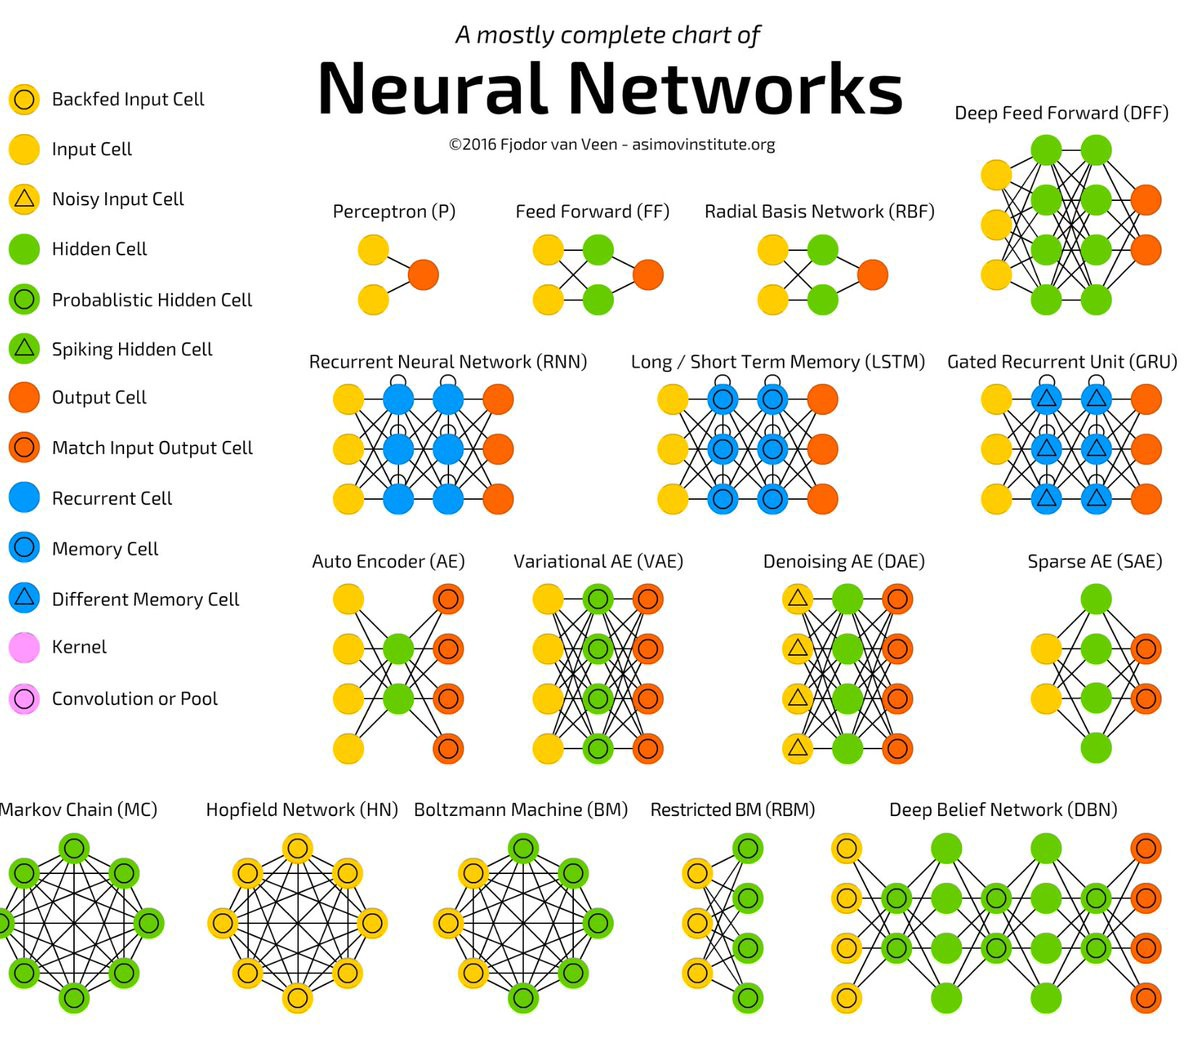
\includegraphics[scale=.2]{figs/neuralNetwork.jpg}
%  \legend{Fonte: GitBook, \cite{exRedeNeural}.}
%  \label{fig:exRedeNeural}
%\end{figure}
%
\begin{figure}[H]
	\centering
	\caption{Exemplo de Redes Neurais}
	\def\svgwidth{14cm}
	\input{figs/svg/neuralNetworksvg.pdf_tex}
	\legend{Fonte: GitBook, \cite{exRedeNeural}.}
	\label{fig:exRedeNeural}
\end{figure}

A figura \ref{fig:iamldl} mostra um exemplo da diferença entre Inteligência Artificial, Machine Learning e Deep Learning, e quando aproximadamente elas começaram a ser abordadas e implementadas.

%\begin{figure}[H]
%  \centering
%  \caption{Diferença entre IA, ML e DL}
%  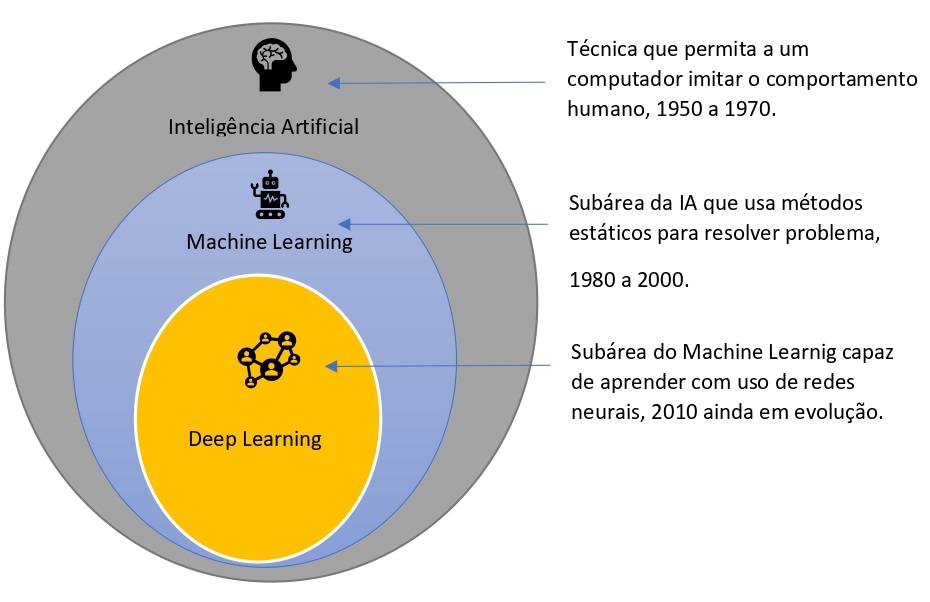
\includegraphics[scale=.7]{figs/IA-ML-DL.jpg}
%  \legend{Fonte: o autor.}
%  \label{fig:iamldl}
%\end{figure}
%
\begin{figure}[H]
	\centering
	\caption{Diferença entre IA, ML e DL}
	\def\svgwidth{15cm}
	\input{figs/svg/ia-ma-dl.pdf_tex}
	\legend{Fonte: o autor.}
	\label{fig:iamldl}
\end{figure}

Uma rede neural nada mais é do que uma maneira de imitar o que ocorre no cérebro humana quando realizamos tarefas e assim ativamos neurônios que por sua vez ativam outros, e assim realizando uma reação em cadeia que gera o que chamamos de pensamento. A figura \ref{fig:neural} é um simples exemplo de uma rede neural em máquinas aonde existem entradas, que ativam neurônios, que por sua vez se ligam com todos os outros neurônios e assim sucessivamente até chegarem em apenas uma saída [20].

%\begin{figure}[htpb]
%  \centering
%  \caption{Rede Neural}
%  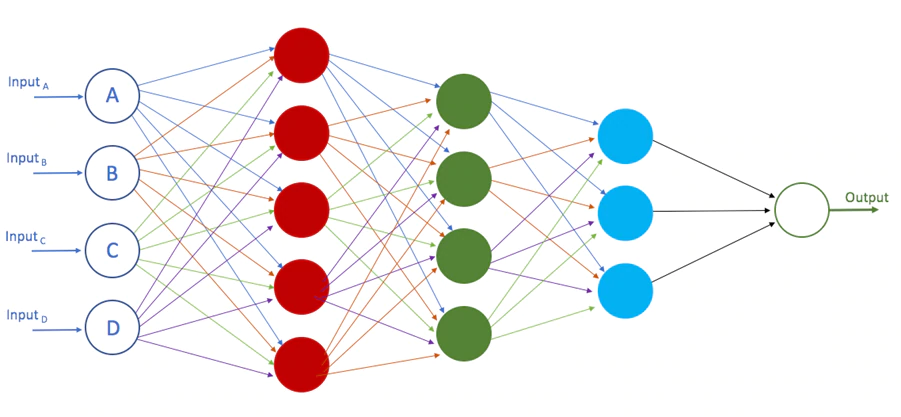
\includegraphics[scale=.5]{figs/neural.png}
%  \legend{Fonte: Oracle. \cite{neural}.}
%  \label{fig:neural}
%\end{figure}
%-
\begin{figure}[H]
	\centering
	\caption{Rede Neural}
	\def\svgwidth{15cm}
	\input{figs/svg/redeneural.pdf_tex}
	\legend{Fonte: o autor com base em Oracle. \cite{neural}.}
	\label{fig:neural}
\end{figure}

\subsection{Visão Computacional}
%-
Visão computacional é um campo da inteligência artificial que treina computadores para interpretar e entender o mundo visual. Através do uso de imagens digitais, câmeras e vídeos junto a modelos de Deep Learning, as máquinas podem identificar e classificar objetos corretamente, e então, reagir ao que elas veem. [10].
Os estudos com visão computacional beiram a época do início da internet, sim isso e verdade já naquela época se estudava este campo, porem tudo era mais difícil, devido à falta de tecnologias para suportar o processamento de grande volume de dados, faltava o volume de dados hoje conhecido como (Big Data) e algoritmos de processamento paralelo [9]. Nessa década vários fatores impulsionam o uso e estudo de visão computacional, tecnologias moveis saturam o mundo com vídeos e fotos o (Big data), o poder computacional cresceu abruptamente e tornou-se mais barato, e novos algoritmos com redes neurais convulsionais aproveitam melhor a capacidade do hardware e do software [10].
 Existem muitos tipos de visão computacional. Hoje no mercado é comum a utilização de algumas tecnologias distintas, tais como:

\begin{itemize}
    \item Segmentação de imagem: Examina uma fração de uma imagem.
    \item Detecção de objetos: Detecta um os mais objetos dentro de um campo de imagem.
    \item Reconhecimento facial: Detecção avançada de objetos que pode distinguir indivíduos.
    \item Deslocamento dinâmico de objetos: Detecta a reorganização de pixels dentro de um campo de imagem (biblioteca NumPy).
\end{itemize}
%-
\subsection{Redes Neurais Profundas (Deep Learning)}
%-
Aprendizagem Profunda ou Deep Learning, é uma subárea da Aprendizagem de Máquina, que emprega algoritmos para processar dados e imitar o processamento feito pelo cérebro humano [9].
Deep Learning nada mais é do que uma evolução das redes neurais, através da utilização de algoritmos de aprendizagem e camadas de aprendizagem cria-se modelos capazes de reconhecer padrões.
Existem várias arquiteturas de redes neurais, uma é a rede neural convolucional profunda demonstrada na figura \ref{fig:neuralConv}, este tipo trabalha muito bem com entrada de dados multidimensional ou espacial que é o caso do tratamento de imagens. 

%\begin{figure}[H]
%  \centering
%  \caption{Rede Neural Convolucional}
%  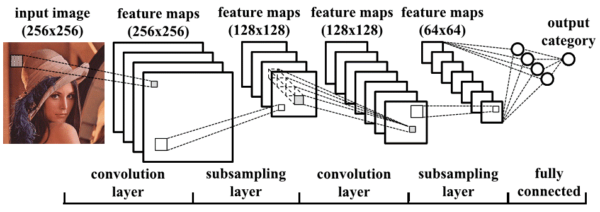
\includegraphics[scale=.6]{figs/neuralConv.png}
%  \legend{Fonte: Lambda3, \cite{neuralConv}}
%  \label{fig:neuralConv}
%\end{figure}
%
\begin{figure}[H]
	\centering
	\caption{Rede Neural Convolucional}
	\def\svgwidth{16cm}
	\input{figs/svg/convolution.pdf_tex}
	\legend{Fonte: o autor com base em Lambda3, \cite{neuralConv}}
	\label{fig:neuralConv}
\end{figure}

Em visão computacional as entradas são matrizes tridimensionais contendo altura e largura e profundidade, o que determina o padrão ou canal de cor do pixel, a figura \ref{fig:pixel} demonstra esse padrão.

%\begin{figure}[htpb]
%  \centering
%  \caption{Pixel em Visão Computacional}
%  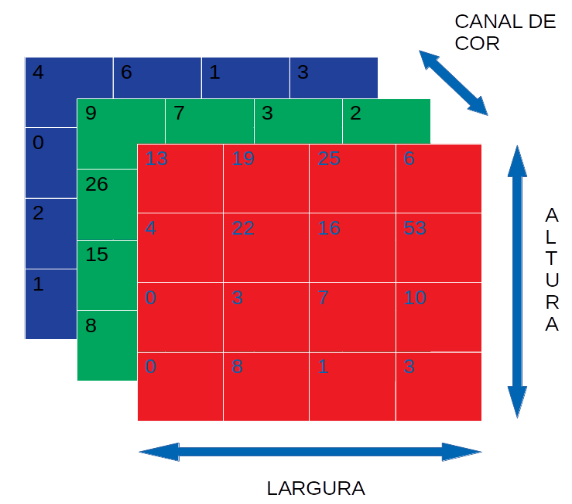
\includegraphics[scale=.9]{figs/pixel.png}
%  \legend{Fonte: o autor.}
%  \label{fig:pixel}
%\end{figure}

\begin{figure}[H]
	\centering
	\caption{Pixel em Visão Computacional}
	\def\svgwidth{10cm}
	\input{figs/svg/pixel.pdf_tex}
	\legend{Fonte: o autor.}
	\label{fig:pixel}
\end{figure}

A primeira coisa que precisamos para treinar um algoritmo de Deep Learning é de uma grande quantidade de imagens (Big data), e através de uma abordagem supervisionada com imagens devidamente marcadas como sendo o rosto que buscamos assim realizamos o treinamento. Então teremos um modelo que recebera imagens não marcadas e ele deverá ser capaz de classificá-las.
%-
\section{Tecnologias Open Source para Tratamento de Imagens}
%\addcontentsline{toc}{section}{Trabalhos Relacionados a Isto}

\subsection{OpenCV}
%-
O OpenCV é uma biblioteca de código aberto licenciada por BSD que inclui várias centenas de algoritmos de visão computacional.
Foi iniciada pela Intel em 1999, é uma biblioteca multiplataforma concentra seu foco no processamento de imagens em tempo real e inclui implementações sem patentes e possui todos os algoritmos mais recentes de visão computacional. Em 2008, a Willow Garage assumiu o suporte e o OpenCV 2.3.1, e ainda possui uma interface de programação para C++, Python e Android.
O OpenCV possui uma estrutura modular, o que significa que o pacote inclui várias bibliotecas compartilhadas ou estáticas [12].
%-
\subsection{Biblioteca Dlib}
%-
O Dlib é um kit de ferramentas de linguagem de programação com licença \textit{Boost Software License} iniciado em 2002 construído em C++ mas extensível para outras linguagens como Python, ela é utilizada largamente na indústria e academicamente para desenvolver sistemas complexos e que envolvam computação de alto desempenho. Hoje em dia ela é desenvolvida para lidar com tráfico de redes, threads, interface gráficas, estrutura de dados, e principalmente em aprendizado de máquina, processamento de imagens, mineração de dados, otimização numérica entre outros [27].
%-
\subsection{Biblioteca Face Recognition}
%-
É uma ferramenta de reconhecimento facial que possui simples utilização sobre a licença \textit{MIT}, construída utilizando a biblioteca de aprendizado profundo de última geração Dlib, ela chega a uma precisão de detecções de até 99,38\% segundo o site \textit{Labeled Faces in the Wild}. É uma ferramenta muito simples de usar por ser baseada em chamadas de funções simples de identificar em sua documentação, porém é uma das melhores ou talvez a melhor ferramenta de detecção facial hoje no mundo.
Com ela é possível não só detectar rostos, mas identificar partes do face como por exemplo; o nariz, boca, olhos, e com algumas outras integrações pode-se até detectar expressões faciais [28].

%-
\subsection{Nvidia Cuda}
%-
No início da computação os computadores sempre operaram com apenas um núcleo programável com códigos executados sequencialmente, porem a demanda por mais desempenho fez com que empresas empregassem esforços para criar tecnologias para melhorar o desempenho, e isso exigiu ainda mais do limite físico do silício. Para contornar isso foram criados os mecanismos de \textit{pipeline}, \textit{threads} e outros, uma alternativa foi adicionar processadores em paralelo e mais atualmente criaram processadores e gpus multicores com vários núcleos em um único chip. Porem foi necessário alterar as técnicas dos códigos que rodavam unicamente em paralelo para aproveitar esses novos recursos.
Em 1999 a empresa americana NVIDIA ao perceber essa demanda por aumento no desempenho e um tipo de processamento específico, lançou sua primeira GPU a GeForce 256, e logo em 2000 criou as GPUs de uso geral (GPGPU).
Inicialmente as GPUs tinham um processamento fixo focada em processamento de gráficos em três dimensões, mas nos últimos anos elas tem melhorado seu hardware focando no aspecto programável, e o resultado disso e uma grande capacidade de processamento focado em aritmética e não só em gráficos.
Hoje as GPUs têm seu processamento focado em gráficos da classe SIMD, são desenvolvidas especificamente para cálculos de pontos flutuantes, usados em renderização de imagens, suas principais características são, massiva capacidade de processamento paralelo, total programabilidade e grande desempenho em cálculos que possua grande volume de dados. Para dominar esse conteúdo programático era necessário um grande conhecimento do desenvolvedor de várias APIs e da arquitetura das placas gráficas além da representação através de coordenadas de vértices, texturas e shaders, aumentando drasticamente o conteúdo programado.
Foi ai que foi desenvolvida a ferramenta NVIDA CUDA em 2006, ela permite ao desenvolvedor uma facilidade ao desenvolver utilizando recursos da GPU sem a necessidade de conhecer a multiplicidade de novos componentes de programação, e utilizando todo o poder de processamento das GPUs, ela também suporta várias linguagens de programação tendo como principais o C++ e o Python.
A biblioteca Dlib utiliza os recursos de processamento do CUDA para melhorar drasticamente o desempenho em processamento e tratamento de imagens, e no treinamento de redes neurais que necessitam de cálculos que possuem grande volume e dados, que seria o caso da detecção facial utilizando redes neurais profundas [29].

%-
\subsection{Reconhecimento Facial}
%-
Já deve ter reparado ultimamente que o  Facebook possui uma grande capacidade de identificar seus amigos em suas fotos, antigamente você mesmo é quem deveria fazer essas marcações, mas agora quando você carrega uma foto, como magica ele marca todos para você, essa técnica se chama reconhecimento facial, é uma tecnologia muito recente e incrível, o FaceBook pode chegar a um acerto de 98\% de precisão \cite{adamgeitgey}.
%-
Apenas reconhecer amigos é muito fácil é uma utilização muito simples para essa incrível técnica, porem no desenvolvimento desse trabalho daremos uma utilização realmente útil para essa tecnologia.
As técnicas de remoção de revestimentos facaias baseados em aprendizado profundo que utilizaremos, são altamente precisas e capazes de serem utilizadas em tempo real. Sera empregado o método de aprendizado métrico profundo "\textit{deep metric learning}” que trabalho com imagens estáticas ou então fluxo de video, a biblioteca de reconhecimento facial (Dlib) gera um vetor de saída conhecido como 128-d, ou seja, ele gera um vetor de tamanho 128 que quantificam a face contendo valores numéricos reais ou pesos como é mais conhecido por quem tem conhecimento na areá. São chamados de pesos porque são eles que indicaram que uma imagem de entrada corresponde a uma pessoas adicionada no banco de imagens da rede neural, e ao comparar esses pesos ira gerar um resultado ou negativa (não é mesma pessoa) ou positivo (é a mesma pessoa). Para treinar uma rede neural utilizando essas técnicas é utilizado o modelo denominado de trigêmeos, para a técnica de reconhecimento facial utilizando aprendizado métrico profundo, envolvera uma etapa de treinamento de trigêmeos. Essa técnica consiste em trés imagens de entrada, aonde ao menos duas das trés são da mesma pessoa, o (NN) gera um vetor de 128-d para cada imagem de rosto, e logo para as duas imagens de mesmo rosto, ajustamos os pesos da rede neural para tornar o vetor o mais próximo possível via métrica de distancia \cite{adriamRF},

%-
%\begin{figure}[htpb]
%  \centering
%  \caption{Exemplo Simples de Treinamento de Rede Neural com Método de Trigêmeos}
%  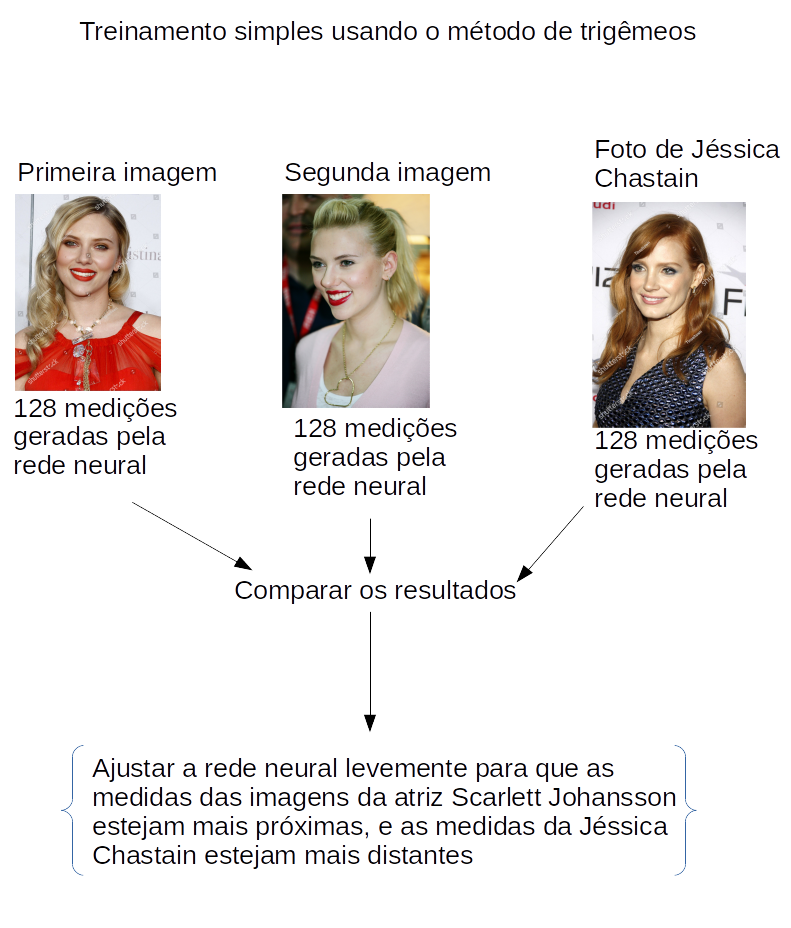
\includegraphics[scale=.4]{figs/atrizes.png}
%  %\includesvg{figs/atrizes.svg}
%  \legend{Fonte: o autor.}
%  \label{fig:treinsimp}
%\end{figure}
%-
\begin{figure}[H]
	\centering
	\caption{Exemplo Simples de Treinamento de Rede Neural com Método de Trigêmeos}
	\fontsize{9pt}{12pt}\selectfont
	\color{black}
	\def\svgwidth{15cm}
	\input{figs/svg/atrizes.pdf_tex}
	\legend{Fonte: o autor com base em \cite{adamgeitgey}.}
	\label{fig:treinsimp}
\end{figure}


Na ilustração \ref{fig:treinsimp} esta uma representação que mostra uma simulação muito simples de como funciona o método com trigêmeos, duas das trés faces são da atriz Scarlet Johansson que sera alvo no reconhecimento facial, e uma foto da atriz Jéssica Chastain que estará no nosso conjunto de dados. Então vamos considerar as faces, logo a ideia geral é que ajustaremos os pesos de nossa rede neural, para que as medias de 128-d das duas fotos da atriz Scarlet Johansson estejam o mais próximas o possível e mais distante da foto da Jéssica Chastain \cite{adamgeitgey}.

A técnica utilizada com a biblioteca (Dlib) e (Face Recognition) é baseada no (ResNet-34) do artigo “\textit{Deep Residual Learning for Image Recognition}” \cite{DBLP:journals/corr/HeZRS15}, mas com menos camadas e a metade do numero de filtros. 

A rede (Dlib) foi criada e treinada por Davis King em um conjunto de aproximadamente 3 milhões de imagens, ela pode chegar a um acerto comparado a outras técnicas de ponta de aproximadamente 99,38\% de precisão, e para concluir ela é uma rede (ResNet) com 29 camadas de convolução \cite{dlib1}.
%-
%\begin{figure}[htpb]
%  \centering
%  \caption{Exemplo de comparação de vetores 128-d}
%  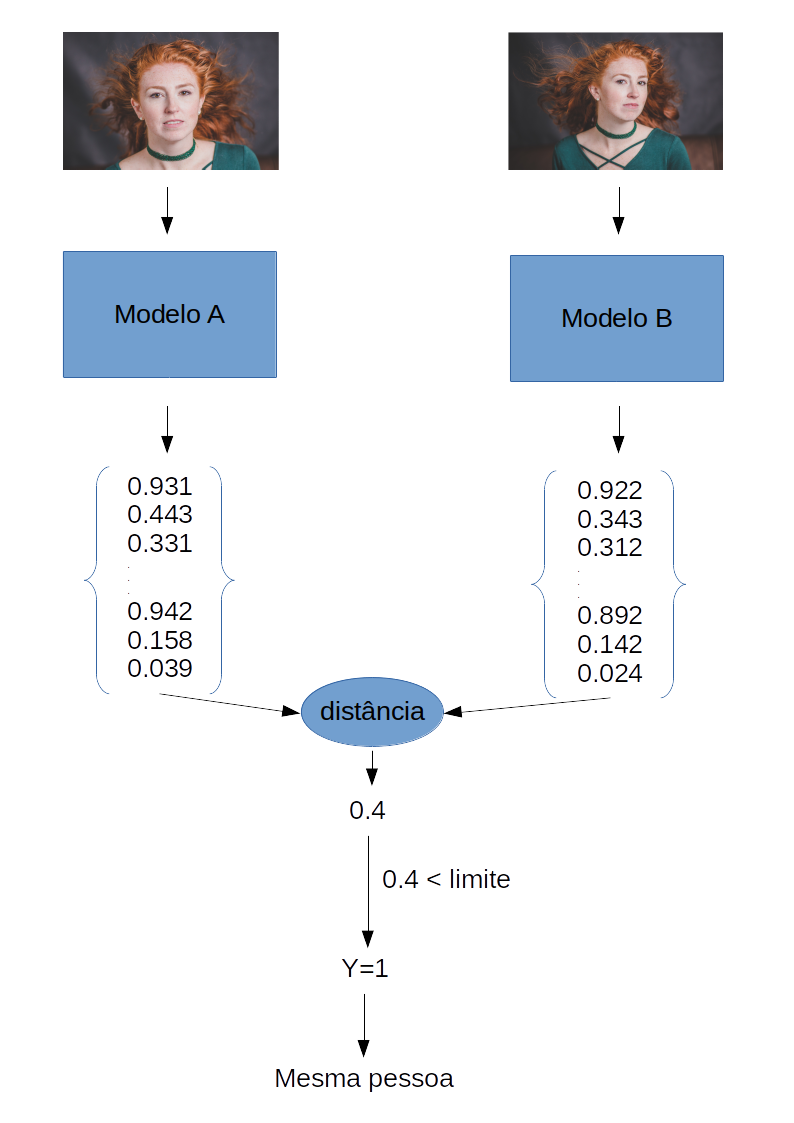
\includegraphics[scale=.5]{figs/gfdg.png}
%  \legend{Fonte: o autor.}
%  \label{fig:exetrein}
%\end{figure}
%-
\begin{figure}[H]
	\centering
	\caption{Exemplo de Comparação de Cetores 128-d}
	\fontsize{9pt}{12pt}\selectfont
	%\color{white}
	\def\svgwidth{13cm}
	\input{figs/svg/metrica.pdf_tex}
	\legend{Fonte: o autor.}
	\label{fig:exetrein}
\end{figure}

A figura \ref{fig:exetrein} é uma representação simples de como se chega a um resultado positivo no reconhecimento facial, como podemos ver os modelos pré-treinados já com seus respectivos pesos de vetores 128-d são comparados, e se perceber os seus valores numéricos são bem próximos, perceba que os valores dentro dos parenteses da direita e esquerda são bem próximos e que o limite é 0,4, logo são comparados e como no exemplo da figura \ref{fig:exetrein} se seu resultado for inferior ao limite estipulado, isso indica que são imagens de uma mesma pessoa, gerando uma saída positiva ou variável Y=1 \cite{adamgeitgey}.

Na figura \ref{fig:ext128d} foi realizada uma simulação utilizando o método de codificação de uma face com reconhecimento facial para extração de um vetor 128-d, e ajustamos o algoritmo para mostrar em tela os pesos que foram encontrados. Ele gera exatamente 128 valores numéricos reais. 

%-
%\begin{figure}[htpb]
%  \centering
%  \caption{Extração de um Vetor 128-d com Reconhecimento Facial}
%  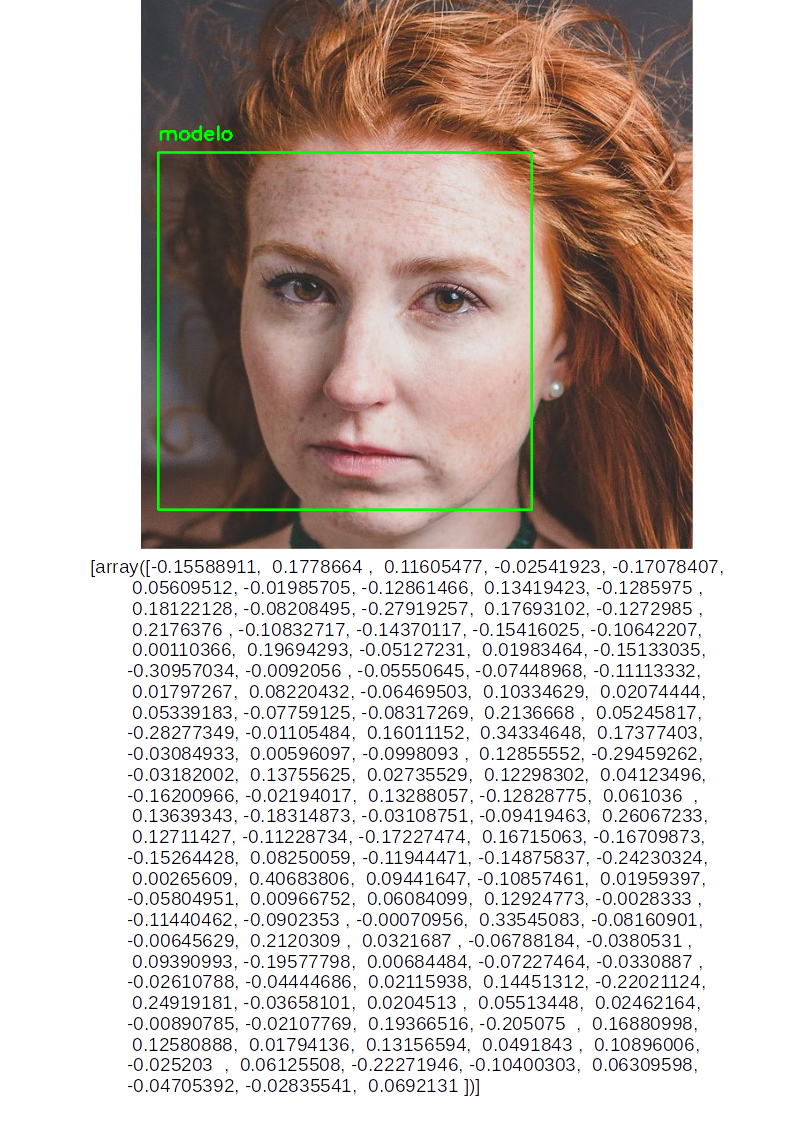
\includegraphics[scale=.5]{figs/modelo.png}
%  \legend{Fonte: o autor.}
%  \label{fig:ext128d}
%\end{figure}
%-
\begin{figure}[H]
	\centering
	\caption{Extração de um Vetor 128-d com Reconhecimento Facial}
	\fontsize{9pt}{12pt}\selectfont
	%\color{white}
	\def\svgwidth{13cm}
	\input{figs/svg/modelo.pdf_tex}
	\legend{Fonte: o autor.}
	\label{fig:ext128d}
\end{figure}

\section{Tecnologias de Linguagem de Programação para Cálculos de Álgebra e Geometria}
%\addcontentsline{toc}{section}{Trabalhos Relacionados a Isto}

\subsection{Biblioteca NumPy}
%-
A biblioteca NumPy é hoje uma das principais ferramentas da linguagem Python utilizadas para cálculos numéricos e estruturas de dados, entre seus recursos ela possui cálculo de matrizes muito rápido e eficiente, funções que manipulam elementos da matriz e entre matrizes, possui ferramentas para leitura e gravação de dados de matrizes em disco, operações de álgebra linear, transformada de Fourier e uma confiável geração de números aleatórios [30]. 
Para o trabalho de movimentação do drone, ou seguir o objeto que será focado como o ator principal do trabalho é necessário saber a posição e coordenadas x e y dos pixels, isso é possível através de cálculos principalmente de matrizes, e para isso o OpenCV suporta a biblioteca NumPy.
 O NumPy é uma biblioteca altamente otimizada para operações numéricas, ele fornece uma sintaxe no estilo MATLAB. Todas as estruturas de matriz do OpenCV são convertidas para matrizes NumPy de e para ela. Portanto, quaisquer que sejam as operações que você possa realizar no NumPy, você pode combiná-lo com o OpenCV, o que aumenta o número de possibilidades. Além disso, várias outras bibliotecas como SciPy, que suporta NumPy podem ser usadas [15]. 

%-
\subsection{Biblioteca SciPy}
%-
A biblioteca SciPy juntamente com a NumPy se tornam uma ferramenta extremamente madura, avançada e confiável para processamento de aplicações cientificas. Há união dela com a NumPy estende muito além os recursos da NumPy, entre os recursos estão; Integração e derivações numéricas, decomposição de matrizes, solucionador de matrizes esparsas, e um grande conjunto de funções para trabalhar com cálculos que envolvem probabilidade e estatísticas. 
Na figura \ref{fig:desl} um breve exemplo de como serão utilizadas essas ferramentas de cálculo no protótipo [30].

%\begin{figure}[htpb]
%  \centering
%  \caption{Exemplo de deslocamento utilizando calculos }
%  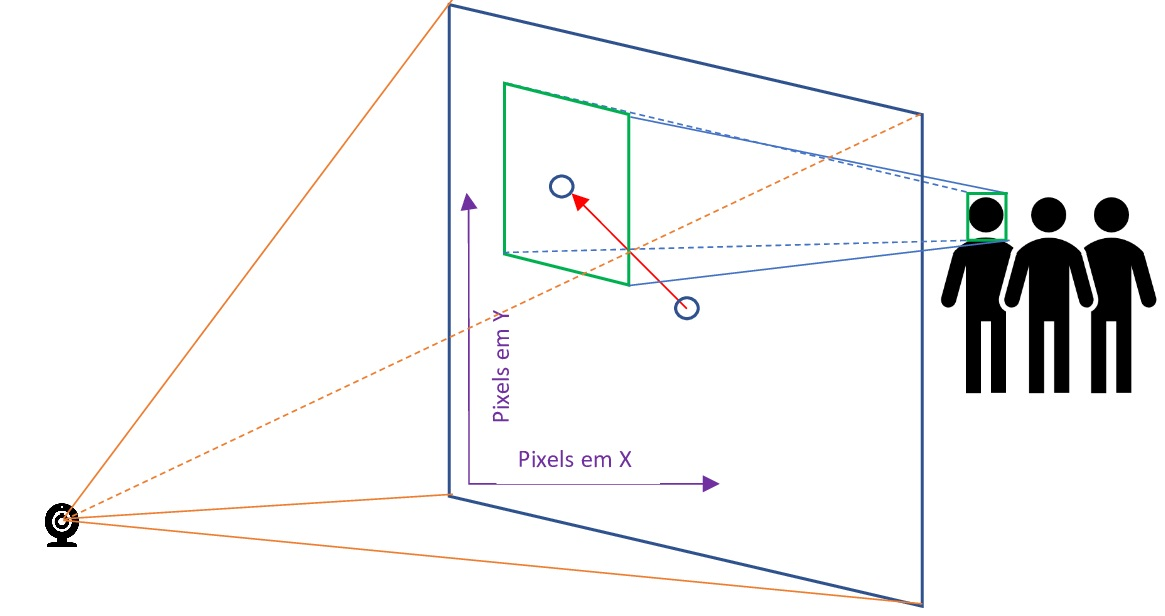
\includegraphics[scale=.5]{figs/rosto.jpg}
%  \legend{Fonte: o autor.}
%  \label{fig:desl}
%\end{figure}
%%-
\begin{figure}[H]
	\centering
	\caption{Exemplo de Deslocamento Dtilizando Dálculos}
	\fontsize{9pt}{12pt}\selectfont
	\color{black}
	\def\svgwidth{15cm}
	\input{figs/svg/rosto.pdf_tex}
	\legend{Fonte: o autor.}
	\label{fig:desl}
\end{figure}

A ideia é através das ferramentas de cálculo das bibliotecas conseguir os valores absolutos em pixels da imagem total captada pela câmera, e do retângulo que é desenhado em volta da face, e através de cálculos descobrir a direção o ângulo e o valor destes vetores direcionais (seta vermelha na figura) e aproximá-los através do deslocamento do drone.

\section{Tecnologias Open Source de Desenvolvimento, para Veículos Aéreos não Tripulados}

\subsection{Firmwares para VANT}

\subsubsection{Ardupilot}
%-
Segundo a site do desenvolvedor, o Ardupilot é o software de piloto automático de código aberto mais avançado, completo e com mais recursos disponíveis. Foi desenvolvido ao longo de mais de 5 anos por uma equipe de diversos engenheiros profissionais e cientistas da computação. É o único software de piloto automático capaz de controlar qualquer sistema de veículo imaginável, de aviões convencionais, multirotores e helicópteros, barcos e até submarinos. E agora sendo expandido para oferecer suporte a novos tipos de veículos emergentes, como quadriciclos e helicópteros compostos [14].
Instalado em mais de um milhão de veículos em todo o mundo e com suas ferramentas avançadas de registro de dados, análise e simulação, o Ardupilot é o software de piloto automático mais testado e comprovado. A base de código-fonte aberto significa que está evoluindo rapidamente, sempre na vanguarda do desenvolvimento da tecnologia. Com muitos fornecedores periféricos criando interfaces, os usuários se beneficiam de um amplo ecossistema de sensores, computadores complementares e sistemas de comunicação. Por fim, como o código-fonte é aberto, ele pode ser auditado para garantir a conformidade com os requisitos de segurança e sigilo [14].
O pacote de software é instalado em aeronaves de muitas empresas como; 3DR, jDrones, PrecisionHawk, AgEagle e Kespry. Também é usado para testes e desenvolvimento por várias grandes instituições e corporações, como NASA, Intel, Boeing, além de inúmeras faculdades e universidades em todo o mundo [14].

\subsubsection{PX4}
\comments{adicionar o firmware px4}

\subsection{Ferramentas de Desenvolvimento para VANT}
%-

\subsubsection{API de Desenvolvimento Dronekit para Ardupilot}
O Dronekit é uma API feita para desenvolvedores criarem aplicativos que se comunicam com veículos (drone) por meio do MAVLink. É uma implementação em linguagem python para o controle de drones através de linguagem de programação, fornece acesso programático as informações de telemetria, estado e parâmetros a veículos conectados, permite o gerenciamento de missões e também o controle direto dos movimentos e operações do veículo.
O uso e direcionado diretamente a mini computadores como Raspberry Pi, Intel Edson, Nvidia TX1 para implementar funções adicionais que a controladora do drone não suporta, entre elas podemos citar a visão computacional e a modelagem 3D. Ele suporta Linux, Mac e Windows e é disponibilizado sobre a licença de código aberto Apache 2.0.

\subsubsection{API de Desenvolvimento MAVSDK para PX4}
%-

\comments{adicionar o mavsdk}

\subsection{Dronekit versus MAVSDK}

\comments{Adicionar uma tabela de comparação entre o dronekit e o mavsdk}

\subsection{Protocolo de Comunicação MAVLink}
%-
E possível criar uma ponte de comunicação entre o computador (Raspberry Pi) e a controladora de voo (Pixhawk), e com ele pode-se capturar pacotes da controladora de voo como por exemplo; registro de telemetria, altitude, velocidade do veículo.
Assim como se consegui capturar informações da controladora de voo, também é possível o contrário ou enviar comandos de voo do computador para a controladora. Todas essas informações trafegam através do protocolo de comunicação MAVLink.
O MAVLink é um protocolo de mensagens muito leve para comunicação em drones (e entre componentes de drones) [13].
O MAVLink segue um moderno padrão de design de publicação-assinatura e ponto a ponto híbrido: Os fluxos de dados são enviados/publicados como tópicos, enquanto os subprotocolo de configuração, como o protocolo de missão ou o parâmetro, são ponto a ponto com retransmissão [13].
As mensagens são definidas nos arquivos XML, cada arquivo XML define o conjunto de mensagens suportado por um sistema MAVLink específico, também conhecido como "dialeto". O conjunto de mensagens de referência implementado pela maioria das estações de controle de solo e pilotos automáticos é definido em common.xml (a maioria dos dialetos é construída sobre essa definição) [13].
A cadeia de ferramentas MAVLink usa as definições de mensagens XML para gerar bibliotecas MAVLink para cada uma das linguagens de programação suportadas. Drones, estações de controle de solo e outros sistemas MAVLink usam as bibliotecas geradas para se comunicar. Eles geralmente são licenciados pelo MIT e, portanto, podem ser usados sem limites em qualquer aplicativo de código fechado sem publicar o código-fonte do aplicativo de código fechado [13].

Características do MAVLink:
Muito eficiente; o MAVLink 1 possui apenas 8 bytes de sobrecarga por pacote, incluindo sinal de início e detecção de queda de pacote. O MAVLink 2 possui apenas 14 bytes de sobrecarga (mas é um protocolo muito mais seguro e extensível). Como o MAVLink não requer nenhum enquadramento adicional, é muito adequado para aplicativos com largura de banda de comunicação muito limitada.
Muito confiável;  MAVLink é usado desde 2009 para se comunicar entre vários veículos, estações terrestres (e outros nós) em canais de comunicação variados e desafiadores (alta latência / ruído). Ele fornece métodos para detectar quedas de pacotes, corrupção e autenticação de pacotes.
Suporta muitas linguagens de programação, executando em vários microcontroladores e sistemas operacionais (incluindo ARM7, ATMega, dsPic, STM32 e Windows, Linux, MacOS, Android e iOS).
Permite até 255 conexões simultâneas na rede (veículos, estações terrestres).
Permite comunicações externas e internas (por exemplo, entre um GCS e um drone, e entre o piloto automático do drone e a câmera do drone habilitada para MAVLink). A figura 6 demonstra o processo de comunicação juntamente com os processos de software, até gerar os dados de saída que são enviados para o drone por protocolo MAVLink.

%-
\subsection{Proxy de Protocolo MAVLink para VANT (MAVProxy)}
%-
O mavproxy e denominado de software para estação terrestre ou (GCS) ground station software, ele é totalmente funcional para o controle de (UAV) unmanned aerial vehicle ou veículo aéreo não tripulado, mas conhecido com drone. Ele foi desenvolvido pela CanberraUAV, é minimalista, portátil e extensível para qualquer UAV que suporte o protocolo MAVlink, visto no índice 2.4.4, um exemplo é o firmware ArduPilot que será abordado mais à frente. Ele foi desenvolvido para suportar computação complementar e vários datalinks, é hoje a ferramenta mais versátil para o controle e desenvolvimento de software baseados em drones, principalmente aqueles direcionados ao Ardupilot. Muitos recursos existentes em outras ferramentas GCS tem sua origem no MAVProxy [25]. O MAVProxy e liberado sobre a licença GNU (general public license) v3 ou superior.
Recursos:
\begin{itemize}
    \item É baseado em linha de comando muito focada em Linux. Existem plugins que fornecem uma GUI (graphical user interface).
    \item Poder ser executado em localhost ou em rede em vários computadores.
    \item Abrange as normas POSIX (portable operating system interface), ou roda em qualquer sistema operacional que tenha chamadas na linguagem python.
    \item Por ser muito leve roda muito bem em computadores com processamento limitado como o Raspberry Pi.
    \item Tab-completion of commands.
    \item Possui módulos carregáveis para várias tarefas como mapas, console, joysticks.
\end{itemize}
%-

\subsection{Simulador de VANT SITL}
%-
O simulador SITL (software in the loop) é uma ferramenta gráfica, no caso ele possui uma GUI (graphical user interface) que implementa a simulação de funcionamento total de um drone, ele permite utilizar um plane (avião), copter (drone) ou um rover (veículo terrestre), e isso sem a necessidade de nenhum hardware, resumindo ele permite testar o comportamento do código desenvolvido com o Dronekit em um simulador de drone assim evitando possíveis imprevistos que poderiam causar algum dano material ao seu equipamento real, seu drone físico. A figura \ref{fig:sitl} mostra um exemplo do simulador rodando em um ambiente Linux, ele demonstra um drone executando um script em python que se chama simple\_goto ou seja o script manda para o console do drone duas coordenadas para a qual ele deve viajar e logo em seguida retornar para a home (ponto de partida).

%\begin{figure}[htpb]
%  \centering
%  \caption{Exemplo de Funcionamento do SITL}
%  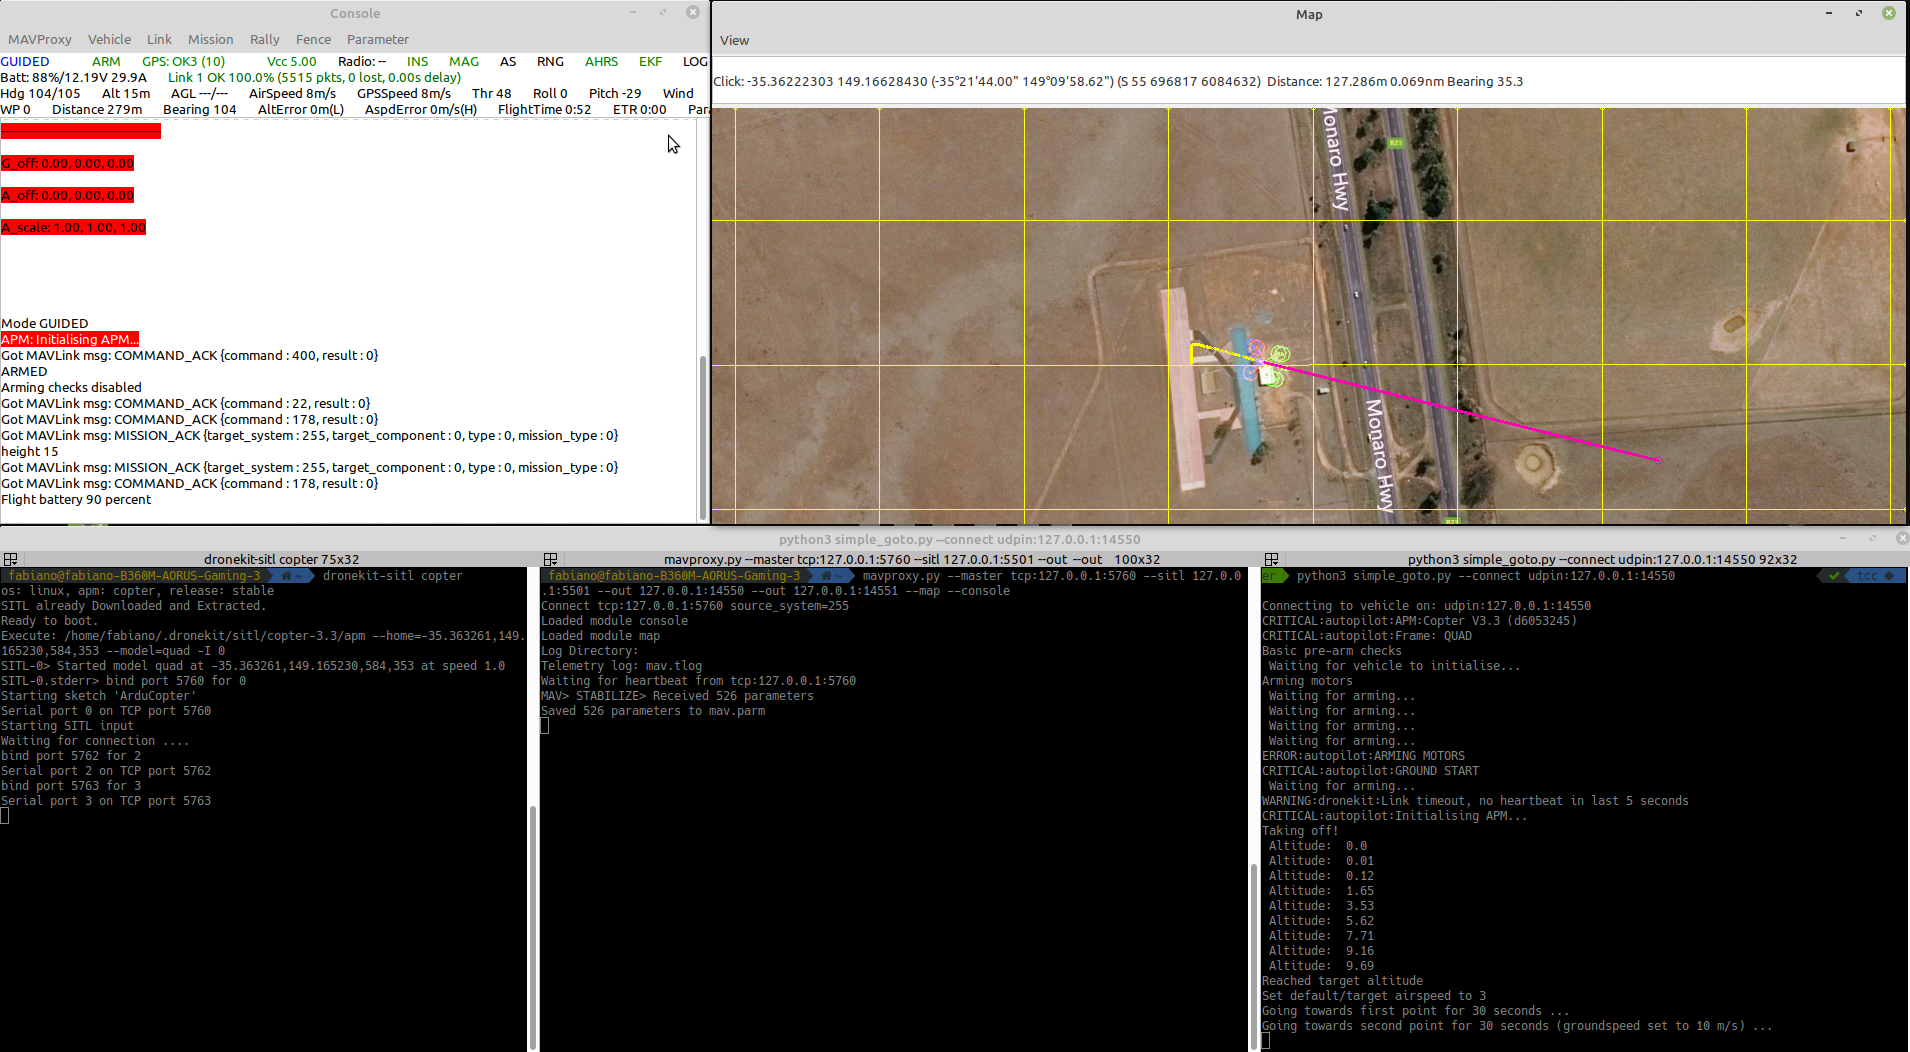
\includegraphics[scale=.3]{figs/sitl.png}
%  \legend{Fonte: o autor.}
%  \label{fig:sitl}
%\end{figure}
%
\begin{figure}[H]
	\centering
	\caption{Exemplo de Funcionamento do SITL}
	\fontsize{9pt}{12pt}\selectfont
	%\color{white}
	\def\svgwidth{15cm}
	\input{figs/svg/sitl.pdf_tex}
	\legend{Fonte: o autor.}
	\label{fig:sitl}
\end{figure}

O SITL permite executar o firmware Ardupilot diretamente no seu computador (nootbook, ou desktop), ele suporta várias plataformas entre elas Linux, Mac e Windows.
Com a junção do SITL e o Ardupilot se tem uma ampla gama de simuladores de veículos embutidos. Por exemplo:
\begin{itemize}
    \item Drone (multi-rotor)
    \item Aeronave de asa fixa
    \item Veículo terrestre
    \item Veículo subaquático
    \item Gimbal para suporte de câmera filmadora
    \item E uma ampla variedade de sensores como, Lidars e sensores óticos
\end{itemize}

Com eles se torna mais fácil o desenvolvimento de aplicativos para drone, isso porque dispõe de uma gama de ferramentas como, analisadores estáticos, depuradores interativos e análise dinâmica. A simulação é uma maneira rápida, fácil e segura de testar códigos implementados para o Ardupilot antes de tentar usar (voar) no mundo real. [26]. A figura \ref{fig:ardupilot} mostra o fluxo de funcionamento das intercomunicações entre os módulos para criar simulações de funcionamento de um drone.

%\begin{figure}[htpb]
%  \centering
%  \caption{Fluxo de operação SITL, MAVProxy, Ardupilot e MAVLink}
%  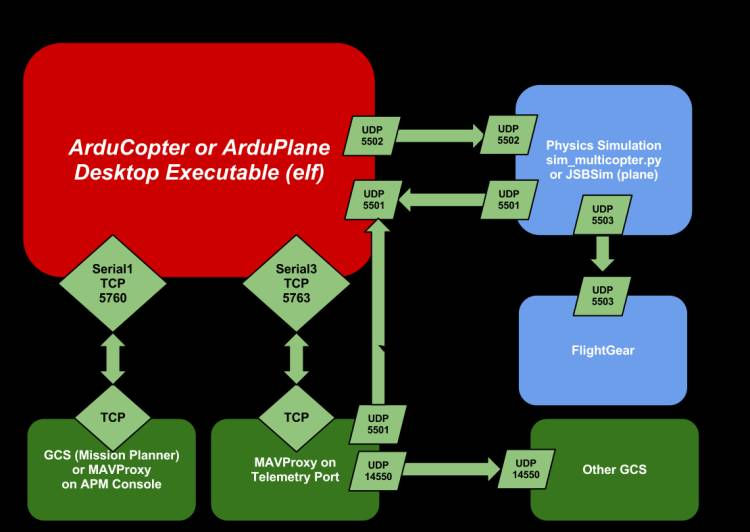
\includegraphics[scale=.5]{figs/ardupilot.jpg}
%  \legend{Fonte: Ardupilot Documents, \cite{ardupilot}}
%  \label{fig:ardupilot}
%\end{figure}
-
\begin{figure}[H]
	\centering
	\caption{Fluxo de Operação SITL, MAVProxy, Ardupilot e MAVLink}
	\fontsize{9pt}{12pt}\selectfont
	\color{white}
	\def\svgwidth{15cm}
	\input{figs/svg/ardupilotsitl.pdf_tex}
	\legend{\color{black}{Fonte: o autor com base em Ardupilot Documents,} \cite{ardupilot}}
	\label{fig:ardupilot}
\end{figure}

%-
\subsection{Simulador de Robótica Gazebo}
%-
O Gazebo é um simulador de código aberto utilizado principalmente em robótica experimental, ele é um simulador muito bem projetado sendo assim tornando possível testar rapidamente algoritmos, projetar robôs, treinar sistema de IA usando cenários extremamente realísticos. O Gazebo possui um poderoso e robusto mecanismo de simulação física, ou seja, simula vários fenômenos físicos como; aceleração da gravidade, temperatura, pressão, luminosidade, e terrenos, também dispões de gráficos de alta qualidade e uma interface gráfica e programática [31]. 
%-
\subsection{Ferramenta para Desenvolvimento de Robótica ROS}
%-
O Ros é um sistema operacional de robótica de código aberto, com ele é possível desenvolver através de linguagem de programação, comportamentos de robôs para serem testados em um simulador como por exemplo o Gazebo. Uma das principais características do ROS e o reuso de código ele disponibiliza diversas aplicações prontas para o uso, essas aplicações simulam variados tipos de robôs, sensores, atuadores, câmeras e muito mais. Ele é implementado unicamente para o sistema operacional Linux, é baseado em versões e uma delas e a Melodic Morenia que é compatível com o Ubuntu Bionic [32].
%-
\section{Tecnologias e a Anatomia de Veículos Aéreos não Tripulados}
%-
Segundo a site do Ardupilot um drone ou multicoptero é um veículo aéreo mecanicamente simples, cujo movimento é controlado pela velocidade ou lentidão de várias unidades de motor/hélice para baixo.
Os multicoptero são aerodinamicamente instáveis e exigem absolutamente um computador de bordo (também conhecido como controlador de voo) para um voo estável. Como resultado, eles são sistemas "Fly by Wire" e se o computador não estiver funcionando, você não estará voando. O controlador de voo combina dados de pequenos giroscópios MEMs, acelerômetros (iguais aos encontrados em smartphones) para manter uma estimativa precisa de sua orientação e posição [14].

%\begin{figure}[htpb]
%  \centering
%  \caption{Drone do Tipo Quadricóptero}
%  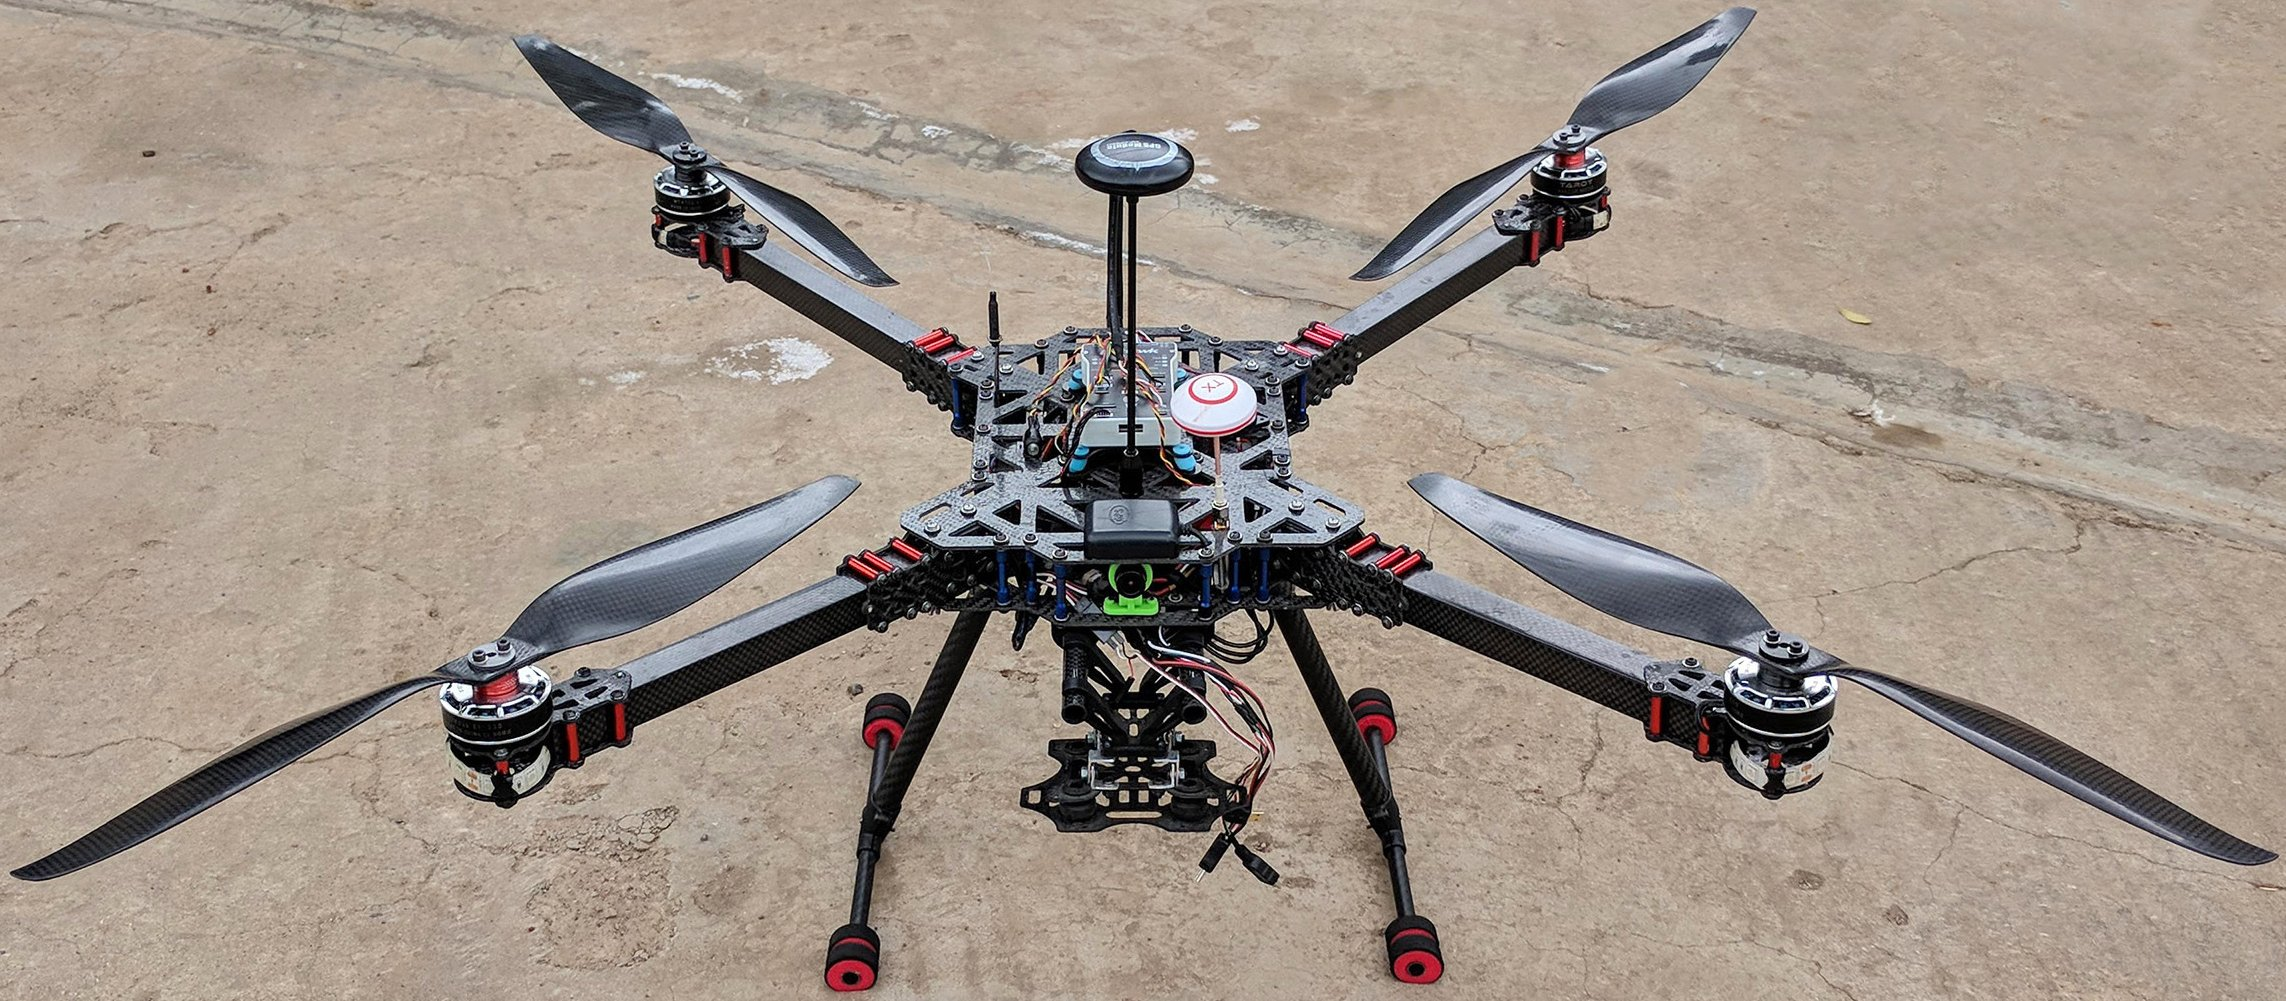
\includegraphics[scale=.2]{figs/drone2.jpg}
%  \legend{Fonte: o autor}
%  \label{fig:quad}
%\end{figure}
%
\begin{figure}[H]
	\centering
	\caption{VANT do Tipo Quadricóptero}
	\fontsize{9pt}{12pt}\selectfont
	%\color{white}
	\def\svgwidth{15cm}
	\input{figs/svg/dronesvgink.pdf_tex}
	\legend{Fonte: o autor}
	\label{fig:quad}
\end{figure}

O drone exemplo na figura \ref{fig:quad}, não será o foco do projeto porem será de importância impactante devido a sua necessidade para que o sistema projetado obtenha todas suas funcionabilidades. No caso do drone ele é o meio de transporte que dará aspecto de mobilidade para que seja possível se deslocar chegando ao foco do escopo, que no caso é seguir o objeto identificado pelo sistema de visão computacional.
Quando tudo estiver em funcionamento, fazendo com que o drone trabalhe de maneira autônoma ele deixara de ser um drone e se tornara um VANT (veículo aéreo não tripulado), e qual a diferença entre eles? Um drone se torna um VANT quando é capaz de vôo autônomo. Normalmente, isso significa pegar as informações de sensores como, acelerômetro e do giroscópio e combiná-las com os dados do barômetro e do GPS, para que o controlador de voo entenda não apenas sua orientação, mas também sua posição.

%-
\subsection{Frame}
%-
O frame é basicamente uma armação que pode ser de plástico, fibra de carbono, fibras entre outros materiais, possui alguns modelos como quadcoptero (quatro hélices), hexacoptero (seis hélices) octacoptero (oito hélices) [3]. A figura \ref{fig:frame} mostra um frame de um quadricóptero.

%\begin{figure}[H]
%  \centering
%  \caption{Frame de um VANT Quadricóptero}
%  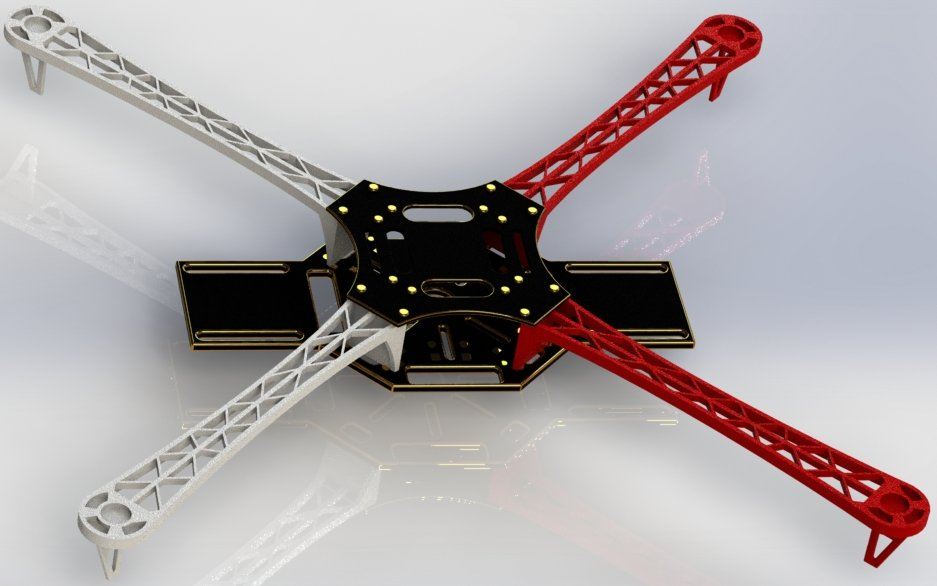
\includegraphics[scale=.5]{figs/frame2.JPG}
%  \legend{Fonte: o autor}
%  \label{fig:frame}
%\end{figure}
%-
\begin{figure}[H]
	\centering
	\caption{Frame de um VANT Quadricóptero}
	\fontsize{9pt}{12pt}\selectfont
	%\color{white}
	\def\svgwidth{13cm}
	\input{figs/svg/frame.pdf_tex}
	\legend{Fonte: o autor}
	\label{fig:frame}
\end{figure}

\subsection{Controladora de Voo}
%-
Uma controladora de voo é um hardware, é basicamente um equipamento físico composto por um circuito integrado o qual possui sensores como barômetro, gps, giroscópio, acelerômetros. Sensores que captam as atividades externas como a pressão do ar, posição geográfica, posição de equilíbrio em relação a gravidade (nivelamento), convertem essas atividades em sinais digitais e dessa forma a controladora juntamente com o firmware (Ardupilot/PX4) que possuem embarcado, conseguem interpretar esses sinais e utilizá-los para que consiga manter o equipamento em equilíbrio no ar, tornando ele um equipamento capaz de voar   e manter sua estabilidade \cite{sete}[7].     
As controladoras de voo ou piloto automático são utilizadas para desenvolver equipamentos de controle remoto como drones, veículos terrestres, aviões e submersíveis aquáticos. Originalmente foram fabricadas e vendido pela 3DR, hoje é possível adquirir copias chinesas com custos bem mais em conta, devido ao projeto ser open source [3].
As figuras \ref{fig:pixhawk} e \ref{fig:pixhawkCirc} mostram a Pixhawk 1 uma das controladoras mais utilizadas.

%\begin{figure}[htpb]
%  \centering
%  \caption{Pixhawk 1}
%  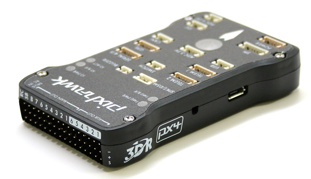
\includegraphics[scale=.7]{figs/pixhawk.png}
%  \legend{Fonte: Ardupilot Documents, \cite{px4}}
%  \label{fig:pixhawk}
%\end{figure}
%
\begin{figure}[H]
	\centering
	\caption{Pixhawk 1}
	\fontsize{9pt}{12pt}\selectfont
	%\color{white}
	\def\svgwidth{13cm}
	\input{figs/svg/pixhaw.pdf_tex}
	\legend{Fonte: Ardupilot Documents, \cite{px4}}
	\label{fig:pixhawk}
\end{figure}

%\begin{figure}[htpb]
%  \centering
%  \caption{Diagrama eletrônico dos conectores da Pixhawk 1}
%  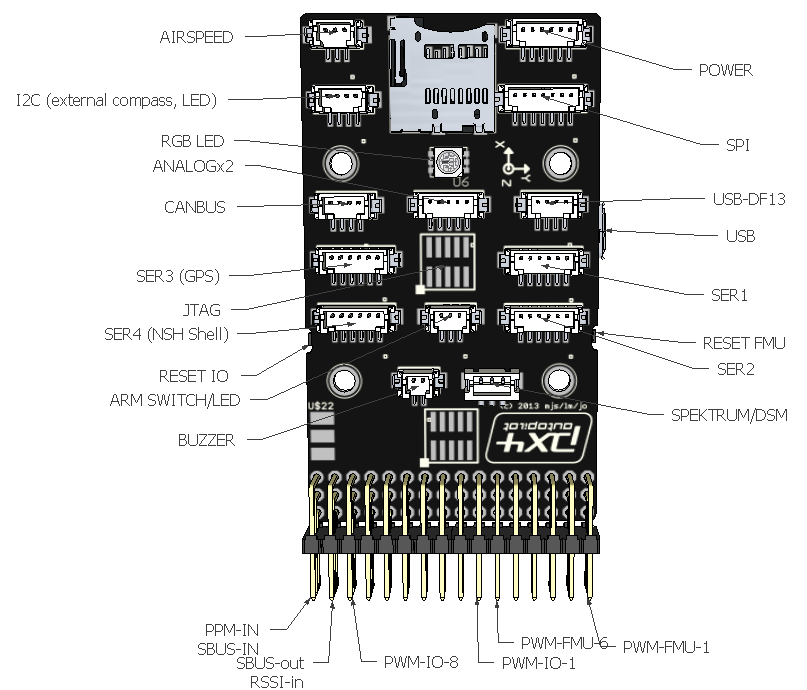
\includegraphics[scale=.4]{figs/Diagrama eletronico pixhawk.png}
%  \legend{Fonte: Ardupilot Documents, \cite{ardupilot}}
%  \label{fig:pixhawkCirc}
%\end{figure}
%
\begin{figure}[H]
	\centering
	\caption{Diagrama Eletrônico dos Conectores da Pixhawk 1}
	\fontsize{9pt}{12pt}\selectfont
	%\color{white}
	\def\svgwidth{13cm}
	\input{figs/svg/Diagrama-eletronico-pixhawk.pdf_tex}
	\legend{Fonte: Ardupilot Documents, \cite{ardupilot}}
	\label{fig:pixhawkCirc}
\end{figure}

\begin{itemize}

    \item Processador:
    \begin{itemize}
        \item Núcleo ARM Cortex M4 de 32 bits com FPU
        \item 168 Mhz / 256 KB de RAM / 2 MB Flash
        \item Co-processador à prova de falhas de 32 bits
        
    \end{itemize}
    
    \item Sensores:
    \begin{itemize}
        \item MPU6000 como principal acelerometro e giroscópio
        \item Giroscópio ST Micro de 16 bits
        \item Acelerômetro / bússola ST Micro de 14 bits (magnetômetro)
        \item Barômetro MEAS
    \end{itemize}
    
    \item Alimentação:
    \begin{itemize}
        \item Controlador de diodo ideal com failover automático
        \item Todas as saídas periféricas protegidas contra sobrecorrente, todas as entradas protegidas contra ESD
    \end{itemize}
    
    \item Interfaces:
    \begin{itemize}
        \item 5x portas seriais UART, 1 com capacidade de alta potência, 2 com controle de fluxo HW
        \item Entrada de Satélite Spektrum DSM / DSM2 / DSM-X
        \item Entrada Futaba S.BUS (saída ainda não implementada)
        \item Sinal de soma PPM
        \item Entrada RSSI (PWM ou tensão)
        \item I2C, SPI, 2x CAN, USB
        \item Entradas ADC de 3.3V e 6.6V
    \end{itemize}
    
    \item Dimensões:
    \begin{itemize}
        \item Peso 38g
        \item Largura 50 mm (2,0 pol.)
        \item Altura 15,5 mm (0,6 pol.)
        \item Comprimento 81,5 mm (3,2 pol.)
    \end{itemize}
     
\end{itemize}
%-
\subsection{Motor sem Escova}
%-
São motores de corrente elétrica continua de baixa tensão e sem escova, são síncronos e para funcionar nescessitam de um (drive) ou inversor de frequência [24]. A figura \ref{fig:motor} mostra um motor e na ilustração \ref{fig:motorpart} as partes internas.
%\begin{figure}[H]
%  \centering
%  \caption{Motor sem Escova}
%  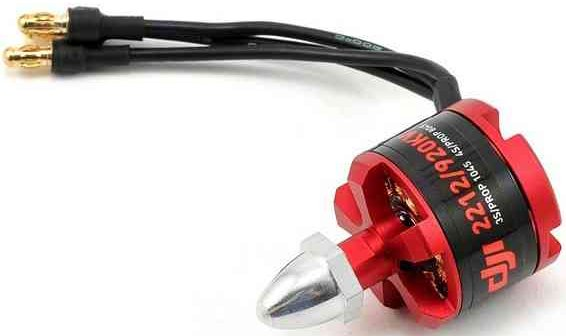
\includegraphics[scale=.3]{figs/brushless_motor.jpg}
%  \legend{Fonte: Ardupilot Documents, \cite{ardupilot}}
%  \label{fig:motor}
%\end{figure}
%
\begin{figure}[H]
	\centering
	\caption{Motor sem Escova}
	\fontsize{9pt}{12pt}\selectfont
	%\color{white}
	\def\svgwidth{13cm}
	\input{figs/svg/brushless_motor.pdf_tex}
	\legend{Fonte: Ardupilot Documents, \cite{ardupilot}}
	\label{fig:motor}
\end{figure}


%\begin{figure}[H]
%  \centering
%  \caption{Partes do Motor}
%  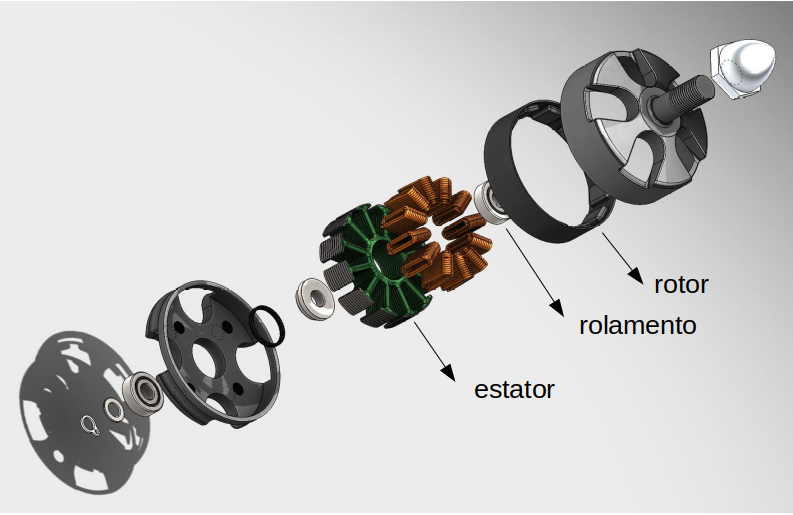
\includegraphics[scale=.4]{figs/motorexp.png}
%  \legend{Fonte: o autor}
%  \label{fig:motorpart}
%\end{figure}
%-
\begin{figure}[H]
	\centering
	\caption{Partes do Motor}
	\fontsize{9pt}{12pt}\selectfont
	%\color{white}
	\def\svgwidth{13cm}
	\input{figs/svg/motorexp.pdf_tex}
	\legend{Fonte: o autor}
	\label{fig:motorpart}
\end{figure}

%-
\subsection{Controlador Eletrônico de Correte (ESC)}
%-
Circuito eletrônico que controla a velocidade de rotação dos motores. A figura \ref{fig:esc} mostra um (ESC) muito utilizado em quadricópteros comuns e na ilustração \ref{fig:motordrive} o diagrama eletrônico.

%\begin{figure}[H]
%  \centering
%  \caption{Controlador Eletrônico de Correte utilizado em VANTs}
%  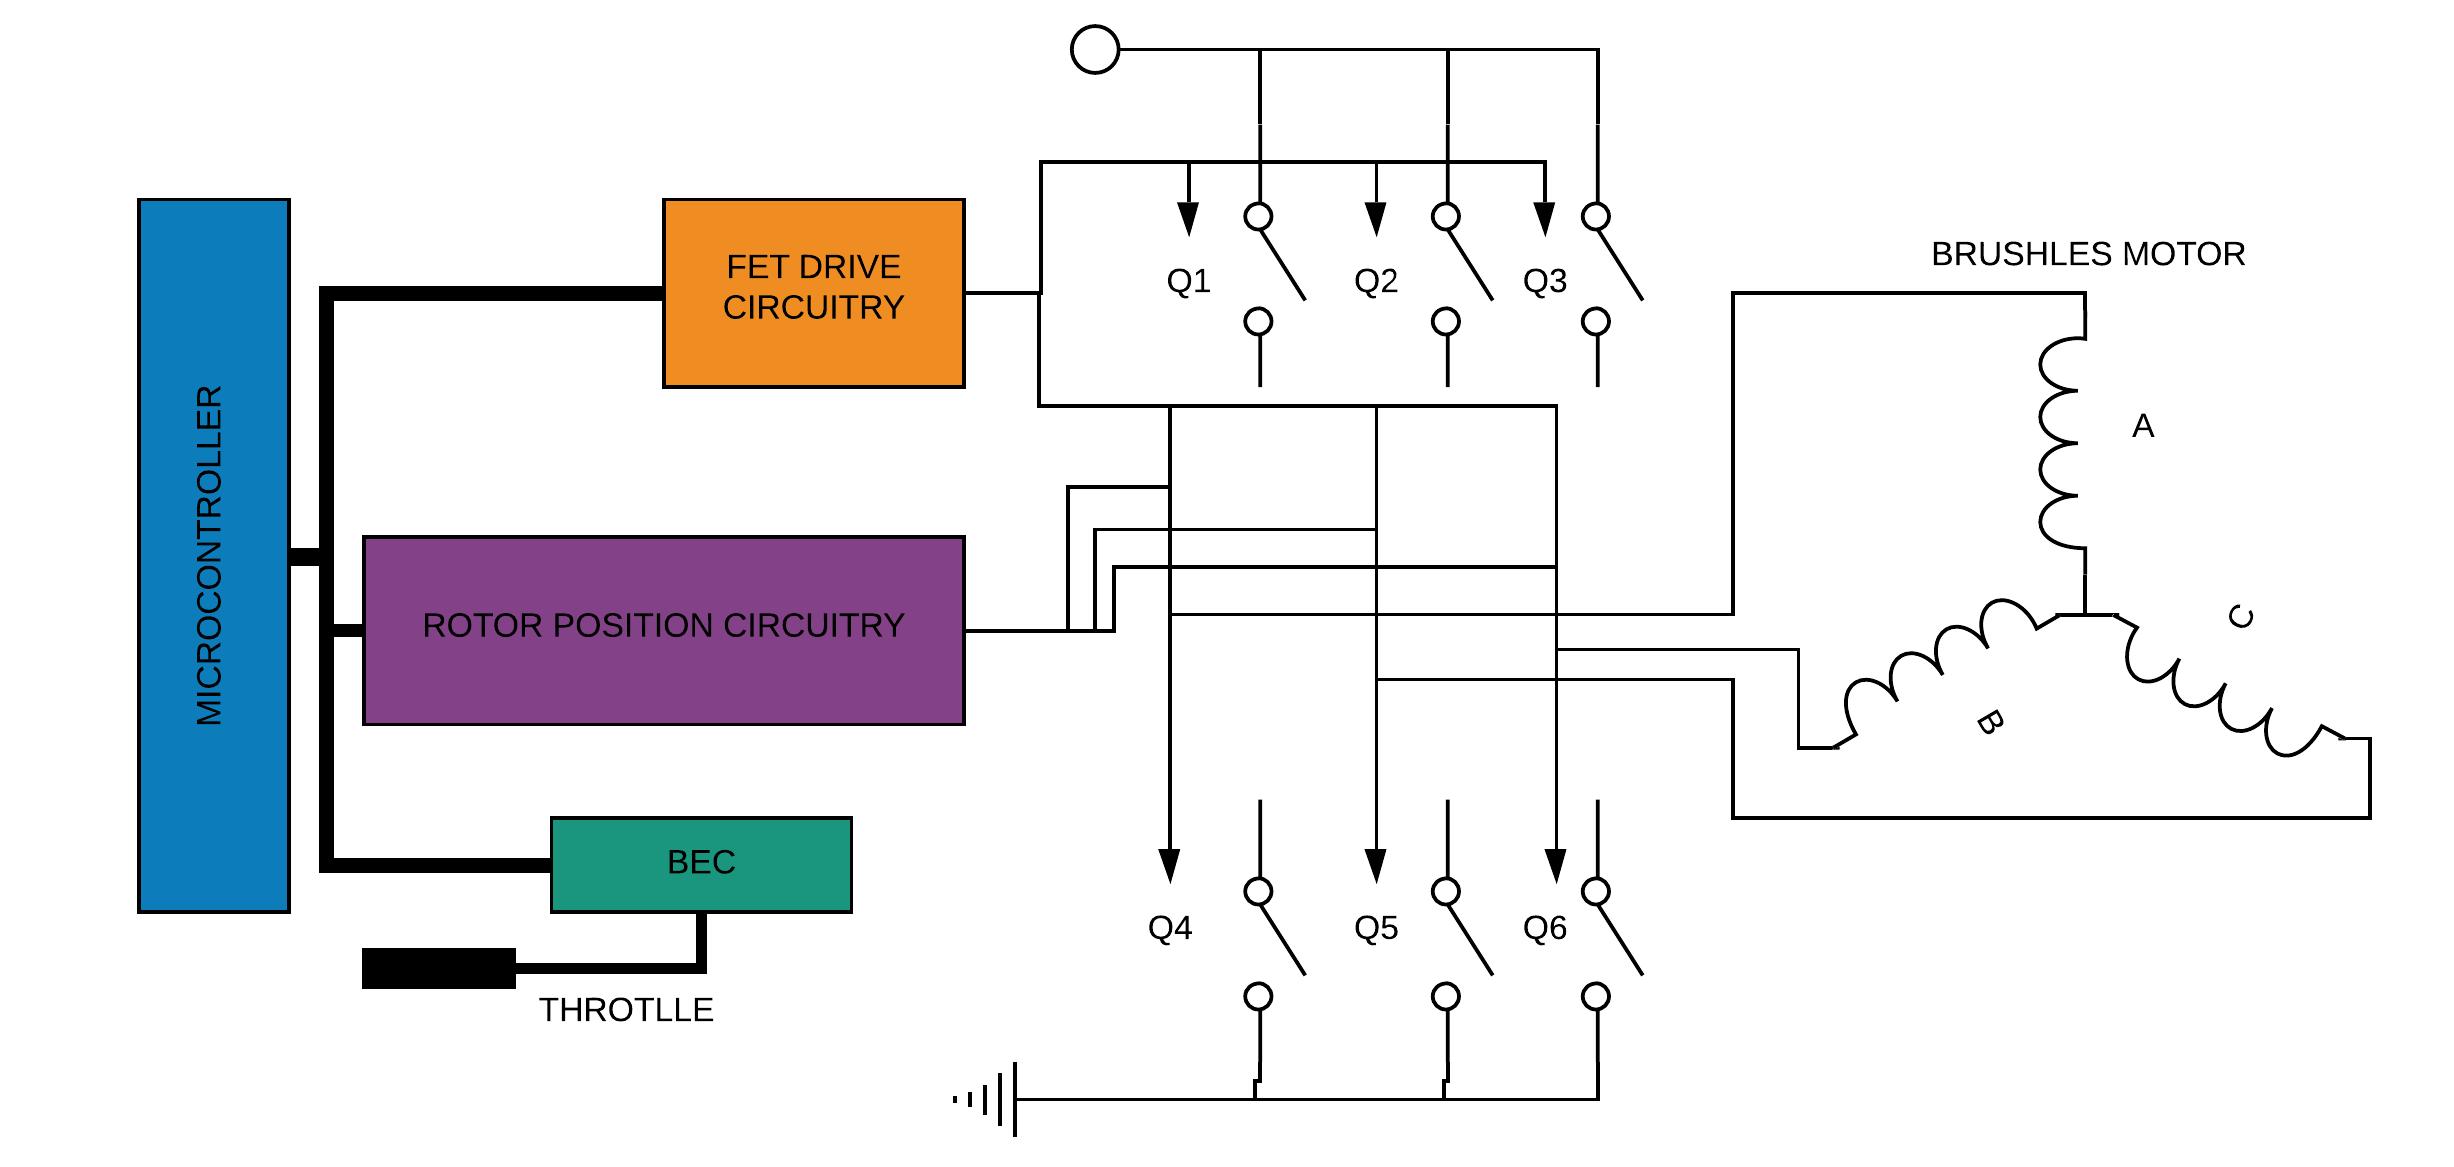
\includegraphics[scale=.18]{figs/drivemotorpng.png}
%  \legend{Fonte: Ardupilot Documents, \cite{ardupilot}}
%  \label{fig:esc}
%\end{figure}
-
\begin{figure}[H]
	\centering
	\caption{Controlador Eletrônico de Correte utilizado em VANTs}
	\fontsize{9pt}{12pt}\selectfont
	%\color{white}
	\def\svgwidth{13cm}
	\input{figs/svg/esc.pdf_tex}
	\legend{Fonte: Ardupilot Documents, \cite{ardupilot}}
	\label{fig:esc}
\end{figure}

\begin{figure}[H]
	\centering
	\caption{Diagrama Eletrônico de um Controlador Eletrônico de Correte}
	\def\svgwidth{15cm}
	\input{figs/svg/drivemotorsvg3.pdf_tex}
	\legend{Fonte: o autor com base em \cite{motordrive}}
	\label{fig:motordrive}
\end{figure}

\subsection{Módulo de GPS}
%-
Módulo de navegação GPS + Compass, é utilizado para a orientação do drone na superfície terrestre. A figura \ref{fig:gps} mostra um modulo de GPS.
%\begin{figure}[H]
%  \centering
%  \caption{Modulo de GPS}
%  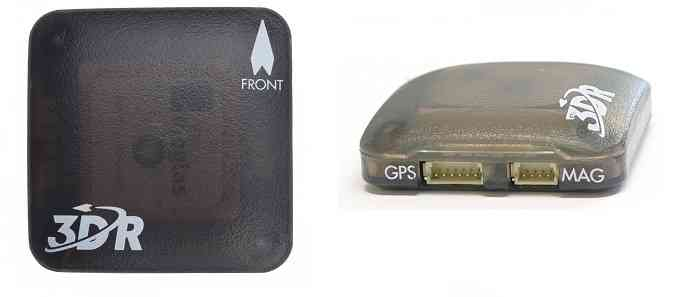
\includegraphics[scale=.8]{figs/gps.jpg}
%  \legend{Fonte: Ardupilot Documents, \cite{ardupilot}}
%  \label{fig:gps}
%\end{figure}
%-
\begin{figure}[H]
	\centering
	\caption{Modulo de GPS}
	\fontsize{9pt}{12pt}\selectfont
	%\color{white}
	\def\svgwidth{15cm}
	\input{figs/svg/gps.pdf_tex}
	\legend{Fonte: Ardupilot Documents, \cite{ardupilot}}
	\label{fig:gps}
\end{figure}

\subsection{Hélice}
%-
E um instrumento de propulsão ou tração, geralmente se acopla a um motor, ao girar empurra o que está na sua volta (ar ou água), assim converte energia rotacional em translacional, empurrando o objeto a que está engatada. Funcionam como asas e obedecem aos princípios de Bernoulli e a terceira lei de Newton. Podem ser fabricadas de resinas, plásticos, fibra de carbono entre outros materiais. A figura \ref{fig:helice} mostra um exemplo de uma hélice.
%\begin{figure}[H]
%  \centering
%  \caption{Hélice}
%  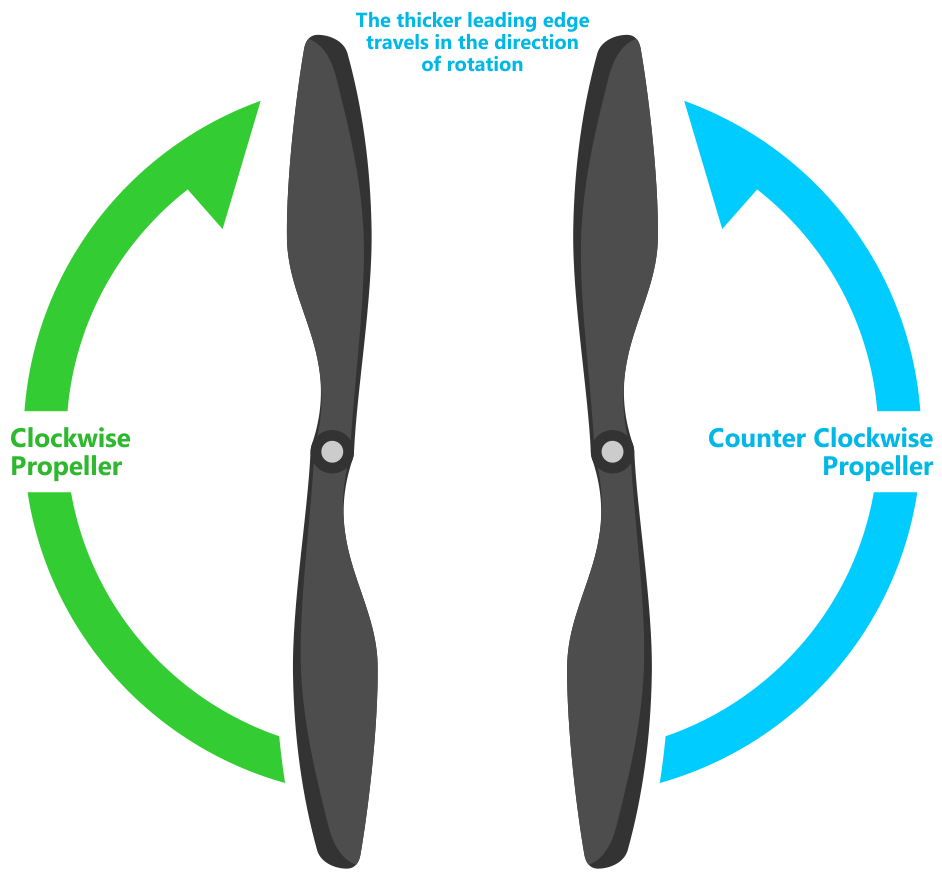
\includegraphics[scale=.7]{figs/helices.png}
%  \legend{Fonte: Ardupilot Documents, \cite{ardupilot}}
%  \label{fig:helice}
%\end{figure}
%-
\begin{figure}[H]
	\centering
	\caption{Hélice}
	\fontsize{9pt}{12pt}\selectfont
	%\color{white}
	\def\svgwidth{13cm}
	\input{figs/svg/helices.pdf_tex}
	\legend{Fonte: Ardupilot Documents, \cite{ardupilot}}
	\label{fig:helice}
\end{figure}

\subsection{Bateria de Polímero de Lítio (LíPo)}
%-
As baterias de polímero de lítio, são baterias que contêm sais de lítio num polímero solido como o oxido de polietileno em vez de solvente, isso as torna adaptáveis ou moldáveis a diferentes formatos. Cada célula tem tensão nominal de 3,7V, sendo que utilizam elas em série chegando a mais de uma especificação de alimentação, exemplo: 2s (duas células), 3s (três células). A figura \ref{fig:bat} mostra uma bateria do tipo LíPo 30c.
%\begin{figure}[H]
%  \centering
%  \caption{Bateria de polímero de lítio}
%  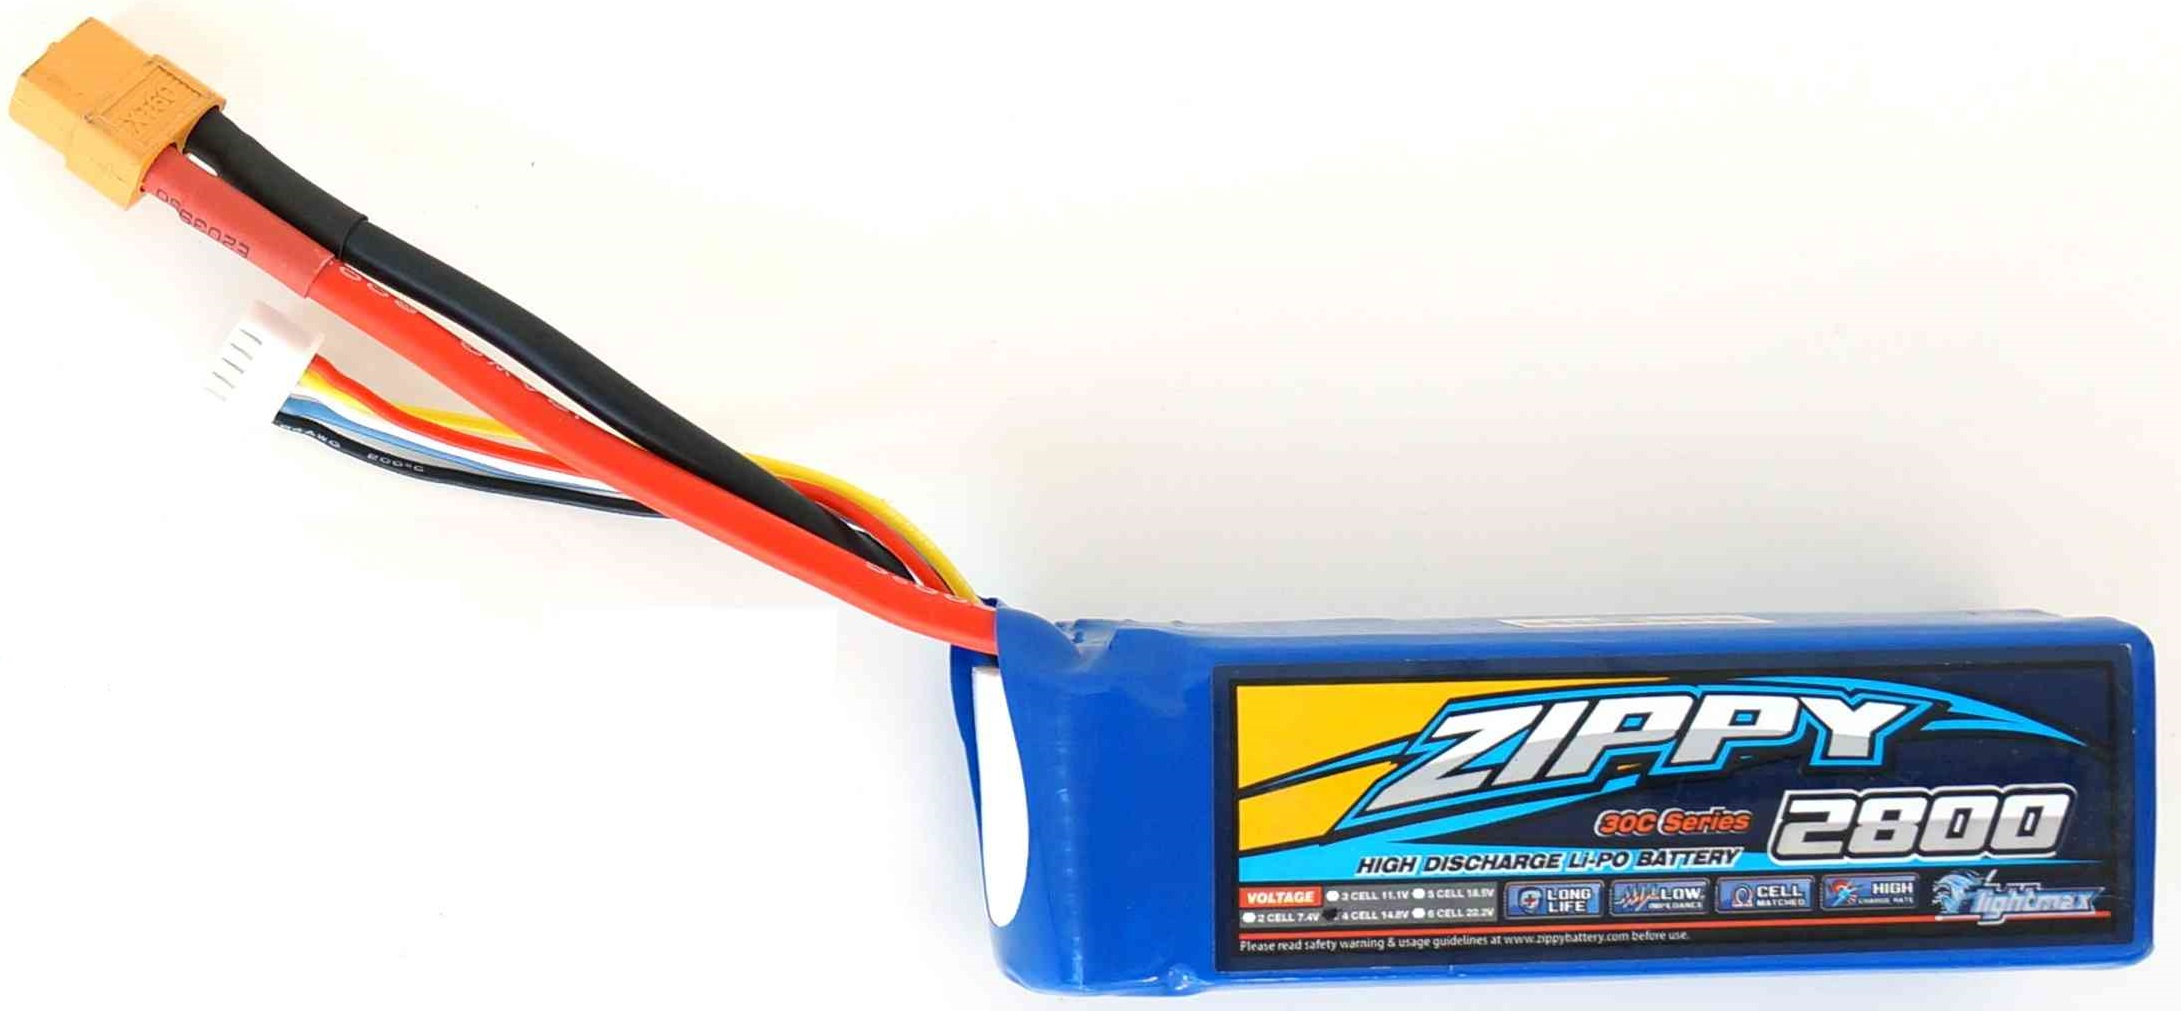
\includegraphics[scale=.2]{figs/bateria.jpg}
%  \legend{Fonte: Ardupilot Documents, \cite{ardupilot}}
%  \label{fig:bat}
%\end{figure}
%-
\begin{figure}[H]
	\centering
	\caption{Bateria de Polímero de Lítio}
	\fontsize{9pt}{12pt}\selectfont
	%\color{white}
	\def\svgwidth{15cm}
	\input{figs/svg/bateria.pdf_tex}
	\legend{Fonte: Ardupilot Documents, \cite{ardupilot}}
	\label{fig:bat}
\end{figure}

\subsection{Esquema de Montagem de um Quadricóptero}
%-
\begin{figure}[H]
  \centering
  \caption{Esquema Básico de Montagem de um VANT do tipo Quadricóptero}
  \fontsize{9pt}{12pt}\selectfont
  \def\svgwidth{15cm}
  \input{figs/svg/esquema-de-ligacao-de-um-drone.pdf_tex}
  \legend{Fonte: do autor}
  \label{fig:esquemamont}
\end{figure}
%-
\section{Teoria de funcionamento e dinâmica de voo de um quadricóptero}

Para iniciar a explicação deste tópico poderíamos começar falando sobre alguma das leis de Newton ou demonstrar através de cálculos que toda a ação possui uma reação de mesma intensidade e diferente direções, porem a ideia é dar uma breve introdução das reações físicas que fazem com que um VANT do tipo quadricóptero voe. 

E para iniciar e preciso entender como uma estrutura do tipo hélice age para que consiga elevar e sustentar o VANT, e para isso será ilustrada a figura \ref{fig:asa} que mostra uma representação gráfica dessas reações. 

%-
%\begin{figure}[htpb]
%  \centering
%  \caption{Teoria de Sustentação de uma Hélice}
%  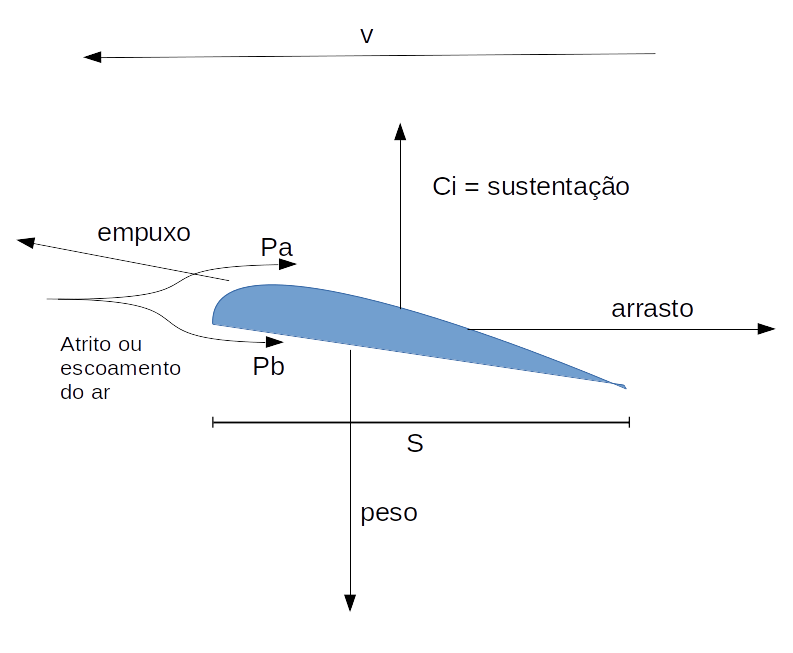
\includegraphics[scale=.4]{figs/helice.png}
%  \legend{Fonte: do autor}
%  \label{fig:asa}
%\end{figure}
%-
\begin{figure}[H]
	\centering
	\caption{Teoria de Sustentação de uma Hélice}
	\fontsize{9pt}{12pt}\selectfont
	%\color{white}
	\def\svgwidth{13cm}
	\input{figs/svg/helice.pdf_tex}
	\legend{Fonte: do autor}
	\label{fig:asa}
\end{figure}

Como pode se ver existem quatro reações principais, o empuxo, sustentação, peso e o arrasto, na figura \ref{fig:asa} Pb e Pa representam a pressão aplicada na hélice, na  parte de baixo da hélice Pb e na parte de cima Pa, essa pressão e exercida pelo deslocamento do ar que passa pela estrutura, basicamente a sustentação e acontece pela diferença de pressão entre Pa e Pb, e o design da estrutura que faz com que a velocidade do ar embaixo da estrutura seja maior do que em cima.

%-
\begin{itemize}
    \item Ci = coeficiente de sustentação;
    \item P = densidade do ar; 
    \item S = areá da superfície da asa;
    \item V = velocidade do ar; 
    \item L = força de sustentação;
\end{itemize}{}
%-
A equação \ref{sust} prova está sustentação: 

\begin{equation}
    \label{sust}
    L=Ci\left(\frac{p}{2}\right)Sv^2
\end{equation}

Existem outras equações matematísticas para calcular outras reações como o arrasto que seria a reação que puxa a estrutura na direção posterior da qual ela quer se deslocar ou então podemos dizer que é o rastro de ar que é deixado pela asa e tenta segura-lo, porem para este projeto é importante saber quais reações criam sustentação e fazem o veículo ganhar altitude vencendo a força da gravidade \cite{inproceedings}.
Agora vamos dar uma olhada nas reações que são aplicadas na estruturo do quadricóptero, como elas reagem juntamente com as reações de momento que a rotação do motor aplicam sobre a estrutura. E para expressar as reações a figura \ref{fig:esfcort} mostra elas graficamente. 

%-
%\begin{figure}[htpb]
%  \centering
%  \caption{Diagrama de Esforços cortantes na Estrutura do Quadricóptero}
%  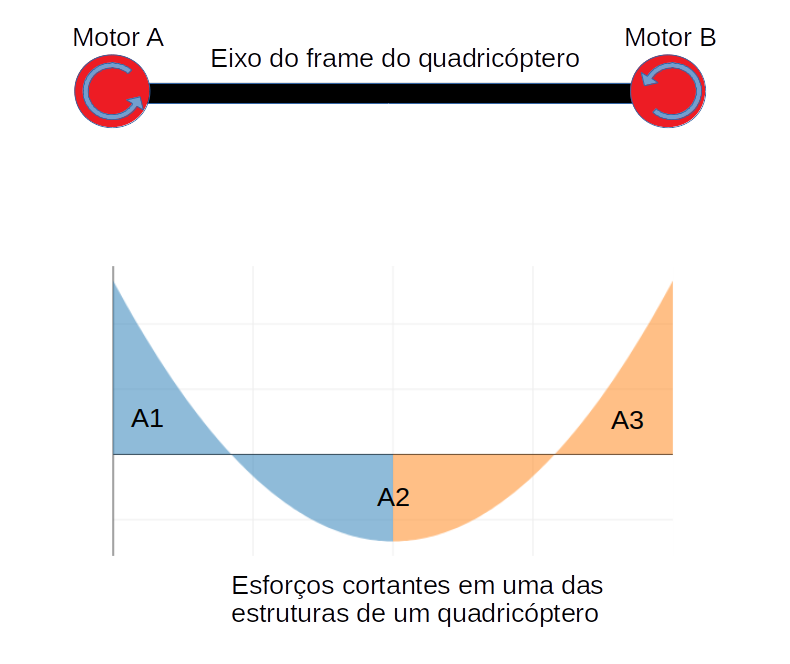
\includegraphics[scale=.3]{figs/esfcortante.png}
%  \legend{Fonte: do autor}
%  \label{fig:esfcort}
%\end{figure}
%-
\begin{figure}[H]
	\centering
	\caption{Diagrama de Esforços cortantes na Estrutura do Quadricóptero}
	\fontsize{9pt}{12pt}\selectfont
	%\color{white}
	\def\svgwidth{13cm}
	\input{figs/svg/esfcortante.pdf_tex}
	\legend{Fonte: do autor}
	\label{fig:esfcort}
\end{figure}

%-
%\begin{figure}[htpb]
%  \centering
%  \caption{Diagrama de Momento Fletor sobre a Estrutura do Quadricóptero}
%  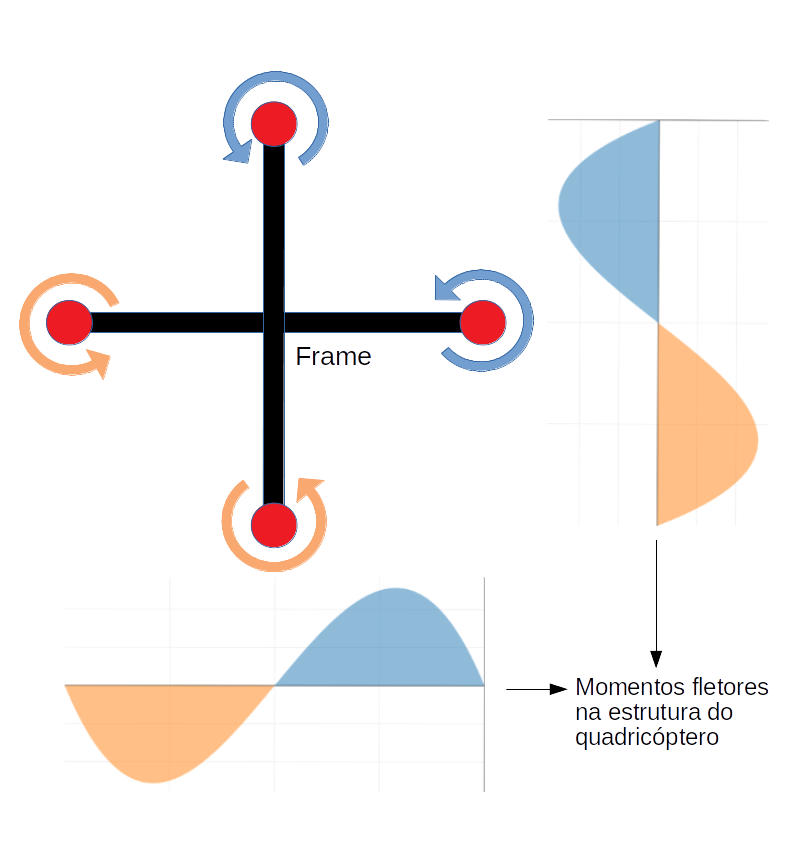
\includegraphics[scale=.3]{figs/momfletor.png}
%  \legend{Fonte: do autor}
%  \label{fig:momflet}
%\end{figure}
%-

\begin{figure}[H]
	\centering
	\caption{Diagrama de Momento Fletor sobre a Estrutura do Quadricóptero}
	\fontsize{9pt}{12pt}\selectfont
	%\color{white}
	\def\svgwidth{13cm}
	\input{figs/svg/momfletor.pdf_tex}
	\legend{Fonte: do autor}
	\label{fig:momflet}
\end{figure}

Na figura \ref{fig:esfcort} as reações que a rotação do motor geram na estrutura no frame dois pontos de esforço cortante, logo e possível observar que elas se cancelam, no caso a areá de  A1=A2 e A3=A2 o que faz com que elas se cancelem e com isso o equipamento não rotacione continuamente em um sentido. Já na figura \ref{fig:momflet} os gráficos de momento fletor demonstram que todas as forças no frame do quadricóptero acabam sempre se anulando. No ponto central do frame do quadricóptero o momento angular é zero dessa forma ele não rotaciona\cite{momesf}. 

%-
%\begin{figure}[htpb]
%  \centering
%  \caption{Sentido de Movimento dos Motores e Inercias}
%  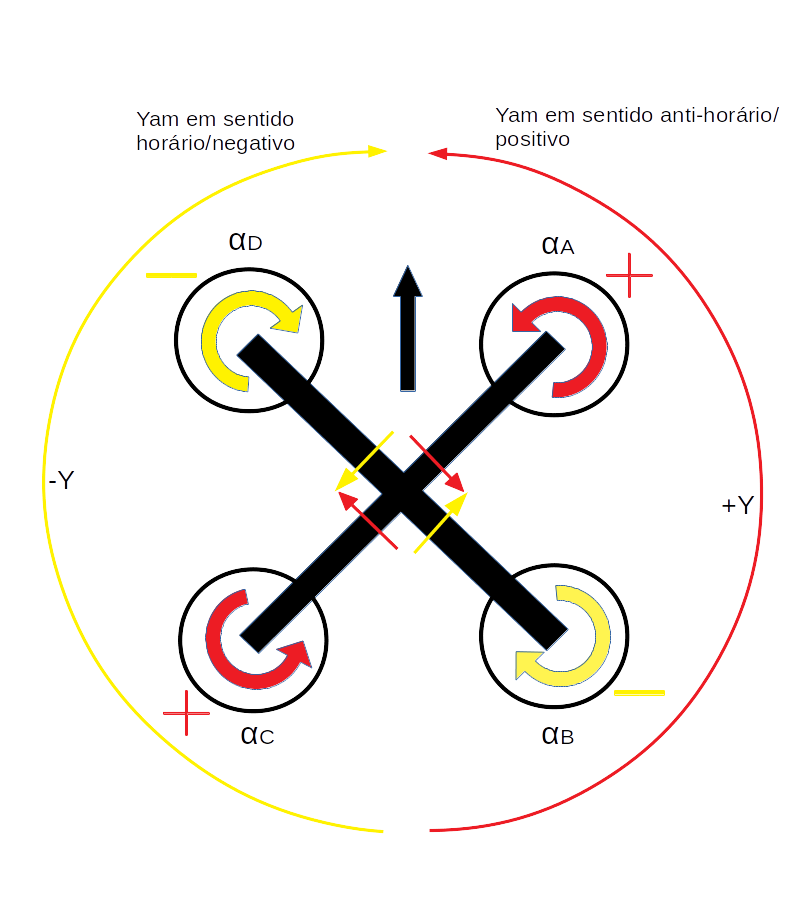
\includegraphics[scale=.3]{figs/rolldrone.png}
%  \legend{Fonte: do autor}
%  \label{fig:rotationmot}
%\end{figure}
%-
\begin{figure}[htpb]
	\centering
	\caption{Sentido de Movimento dos Motores e Inercias}
	\fontsize{11pt}{14pt}\selectfont
	%\color{white}
	\def\svgwidth{13cm}
	\input{figs/svg/rolldrone.pdf_tex}
	\legend{Fonte: do autor}
	\label{fig:rotationmot}
\end{figure}

No plano vertical um quadricóptero pode subir, descer e pairar, com isso é possível deduzir que para subir serão aplicadas forças nos motores de maneira que crie uma força ascendente que supere seu peso, e logo para pairar essas forças precisam se igualar ao máximo possível, mas tendo em mente que se igualarem é fisicamente impossível devido as varias reações da física que são exercidas no quadricóptero, logo para descer ele deve diminuir a velocidade de rotação dos motores de maneira que ascenda lentamente devido ao seu peso exercer empuxo gravitacional. 

Na pratica isso é simples os rotores giram jogando ar para baixo o ar empurra o equipamento para cima, e quem faz com que ele fique nivelado é a controladora de voo que simultaneamente com os sensores inerciais controlam a inclinação aplicando mais potência para cada motor independente de maneira que ele fique nivelado com a gravidade da terra, sim isso acontece muito rápido e freneticamente não é perceptível a olho nu \cite{forcecontrol}. 

Até aqui já sabemos como o quadricóptero sobe, desce,e paira, também sabemos o porque dele não girar em apenas um sentido, agora sera abordada a dinâmica do quadricóptero, ação que faz do quadricóptero um equipamento incrível, tendo capacidade de se movimentar rapidamente e em direções variadas, para quem não sabe é possível realizar uma manobra de "\textit{loop}" ou "\textit{flip}", é a capacidade de dar um giro muito rápido virando de ponta cabeça e voltando rapidamente a posição inicial. 

A figura \ref{fig:yamrollpitch} mostra todos os movimentos e seus respectivos nomes assim como são conhecidos, o "\textit{yam}" é o giro que o quadricóptero da em cima do seu próprio eixo pode ser em sentido horário e antiaéreo, "\textit{roll}" é uma inclinação lateral em relação a frente fazendo com que ele vá para a direita ou esquerda e logo o "\textit{pitch}" é a inclinação que faz com que ele se desloque na direção frontal ou traseira. 

%-
%\begin{figure}[htb]
%  \centering
%  \caption{Movimentos de um Quadricóptero}
%  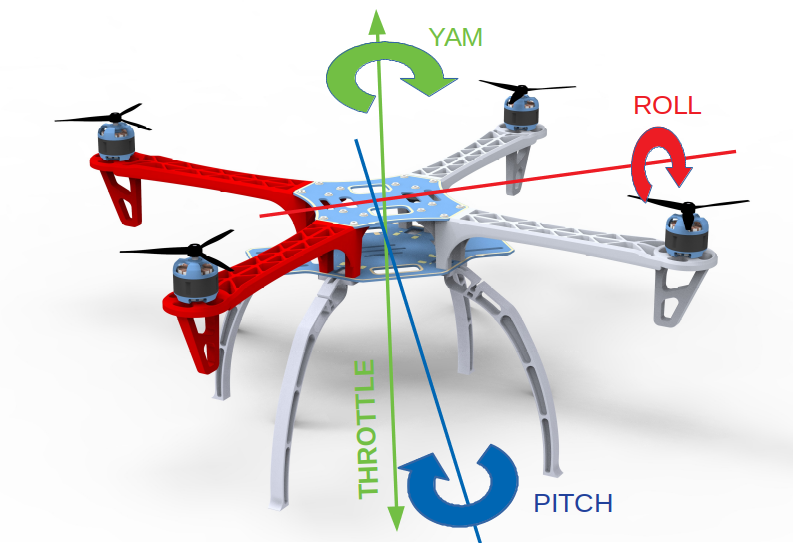
\includegraphics[scale=.3]{figs/F450.png}
%  \legend{Fonte: do autor}
%  \label{fig:yamrollpitch}
%\end{figure}
%-
\begin{figure}[H]
	\centering
	\caption{Movimentos de um Quadricóptero}
	\fontsize{9pt}{12pt}\selectfont
	%\color{white}
	\def\svgwidth{15cm}
	\input{figs/svg/F450.pdf_tex}
	\legend{Fonte: do autor}
	\label{fig:yamrollpitch}
\end{figure}

O VANT de quatro hélices possui basicamente dois movimentos que estimulam deslocamento, um deles é a guinada que faz com que ele se desloque horizontalmente dentro do plano cartesiano, já o movimento de giro ele rotaciona mudando a sua posição frontal e traseira respectivamente, muda o sentido de orientação da frente do equipamento como por exemplo de norte para leste e o sensor que rege esse movimento é a bussola do modulo de GPS. O movimento de giro acontece alterando a rotação dos motores, dois ao mesmo tempo no caso, um exemplo é como rotacionar ele no sentido horário. Perceba que na figura \ref{fig:rotationmot} $\alpha_{D}$ e $\alpha_{B}$ são negativos e $\alpha_{A}$ e $\alpha_{C}$ positivos, logo se atribuirmos a $\alpha_{D}$ e $\alpha_{A}$ um valor numérico 2 e a $\alpha_{C}$ e $\alpha_{B}$ o valor 2 igualmente chegaremos a um resultado zero o que indica que o VANT esta pairando sem girar.  

A soma dos torques dos motores gera a equação \ref{yam} que rege o movimento de Yam. 

\begin{equation}
    \label{yam}
    \left(k\right)\left(\alpha_{D}+\alpha_{A}-\alpha_{C}-\alpha_{B}\right)=Yd^2\left(\frac{\theta Y}{dt^2}\right)
\end{equation}

Vamos realizar outro exemplo de movimento, vamos supor que por exemplo queira girar para esquerda, segundo a figura \ref{fig:rotationmot} e a equação \ref{yam} atribuiremos para $\alpha_{C}$ e $\alpha_{A}$ o valor 3 e a $\alpha_{D}$ e $\alpha_{B}$ o valor 1, então chegaremos novamente a zero o que indica que o VANT esta estabilizado, porem a maior propulsão nos motores $\alpha_{B}$ e $\alpha_{D}$ faz com que ele gire no sentido anti-horário ou seu Y sera negativo como a ilustração \ref{fig:rotationmot} mostra \cite{momesf}.

A mesma equação apenas com uma pequena alteração pode ser aplicada para criar o movimento horizontal conhecido com "\textit{roll}". 

A soma dos momentos no centro de massa gera a equação \ que rege "\textit{roll}". 

\begin{equation}
    \label{roll}
    Lk\left(k\right)\left(\alpha_{D}+\alpha_{A}-\alpha_{C}-\alpha_{B}\right)=Rd^2\left(\frac{\theta R}{dt^2}\right)
\end{equation}

%-
%\begin{figure}[htb]
%  \centering
%  \caption{Movimento horizontal "\textit{roll}"}
%  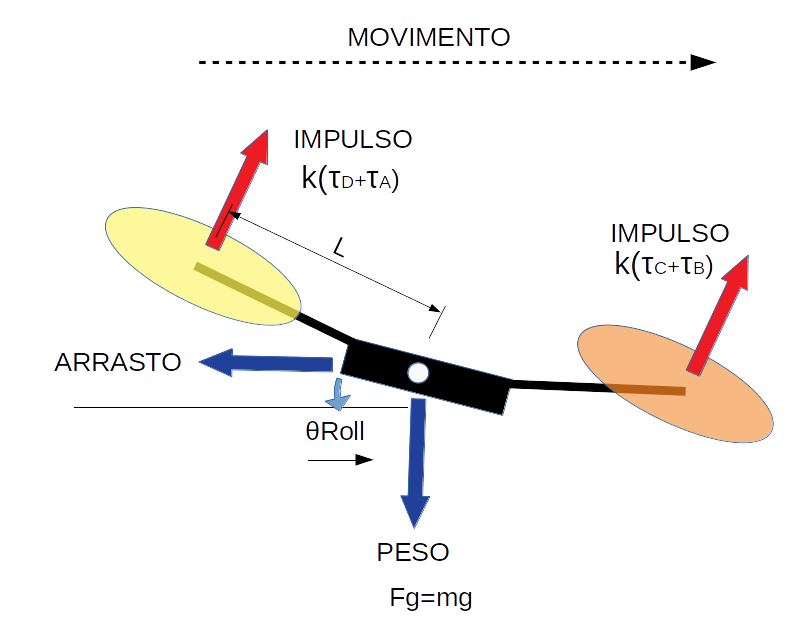
\includegraphics[scale=.3]{figs/dirdrone.png}
%  \legend{Fonte: do autor}
%  \label{fig:roll}
%\end{figure}
%-
\begin{figure}[H]
	\centering
	\caption{Movimento Horizontal "\textit{Roll}"}
		\fontsize{9pt}{12pt}\selectfont
	%\color{white}
	\def\svgwidth{15cm}
	\input{figs/svg/dirdrone.pdf_tex}
	\legend{Fonte: do autor}
	\label{fig:roll}
\end{figure}

A figura \ref{fig:roll} ilustra uma vista lateral do movimento horizontal "\textit{roll}" e forças que o regem, perceba que o VANT esta inclinado mas como se consegue coloca-lo nesta posição? O aumento do impulso nos motores $\alpha_{C}$ e $\alpha_{B}$ e diminuição nos motores $\alpha_{D}$ e $\alpha_{A}$. O impulso total continua igual zero ou seu momento angular resulta em zero, porem a inclinação faz com que ele vá na direção em que esta inclinado, e a equação \ref{roll} e quem define esse movimento horizontal.
E para concluir a ilustração \ref{fig:dirdrone} denomina todos os movimentos horizontais de um quadricóptero \cite{calcmov}.  

%-
%\begin{figure}[htb]
%  \centering
%  \caption{Movimentos horizontais de um quadricópter }
%  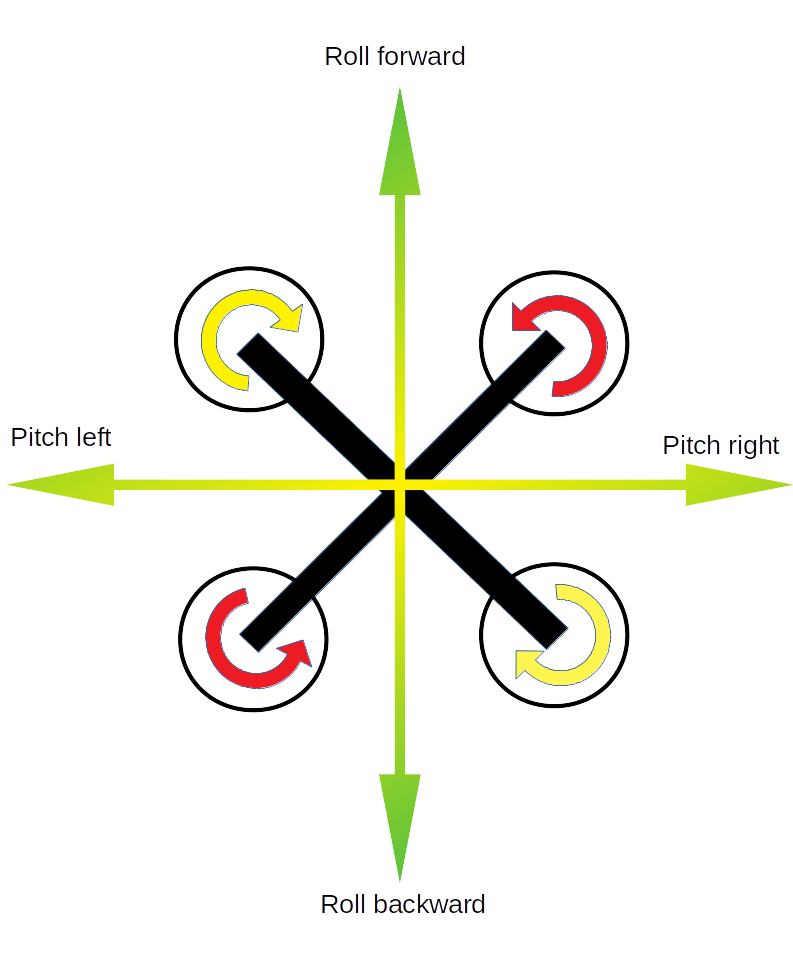
\includegraphics[scale=.3]{figs/sentido.png}
%  \legend{Fonte: do autor}
%  \label{fig:dirdrone}
%\end{figure}
%-
\begin{figure}[H]
	\centering
	\caption{Movimentos Horizontais de um Huadricóptero}
	\fontsize{9pt}{12pt}\selectfont
	%\color{black}
	\def\svgwidth{15cm}
	\input{figs/svg/sentido.pdf_tex}
	\legend{Fonte: do autor}
	\label{fig:dirdrone}
\end{figure}

Para orientar-se e se deslocar na superfície terrestre o VANT se orienta pelo sistema NED (North, East ,Down) que se baseia nos "cálculos de coordenadas do plano tangencial", o qual equaciona como um plano se desloca por uma superfície esférica, sendo regido e se parecendo com a equação \ref{tang}. Isso é um conteúdo de geometria analítica e não é de difícil entendimento sendo encontrado em qualquer material de álgebra básica e para melhor entendimento a ilustração \ref{fig:planacart} foi adicionada.  

\begin{equation}
	\label{tang}
	PT=a\left(x-x0\right)+b\left(y-y0\right)+c\left(z-z0\right)
\end{equation}

\begin{figure}[H]
	\centering
	\caption{Plano Cartesiano na Superfície Esférica}
	\fontsize{9pt}{12pt}\selectfont
	\color{black}
	\def\svgwidth{15cm}
	\input{figs/svg/planocart.pdf_tex}
	\legend{Fonte: do autor}
	\label{fig:planacart}
\end{figure}

Como foi abordado o VANT se orientar usando o sistema de coordenadas NED aonde N é o eixo Norte e Leste D é um eixo que aponta para baixo do VANT chegando próximo ao centroide da terra, são vetores de orientação usados na aviação aérea e cibernética marinha. Ele é usado comumente em sistemas GPS para movimentar-se ao redor do globo e são tangentes as linhas das coordenadas geográficas. A ilustração \ref{fig:ned} mostra graficamente todas as referencias entre o frame de um VANT com o sistema de coordenadas:

\begin{itemize}
	\item A tangente Leste-Oeste em paralelo com os paralelos;
	\item A tangente Norte-Sul em paralelo com os meridianos;
\end{itemize}

Também é possível observar na ilustração \ref{fig:ned} como funciona o sistema de orientação do Dronekit e do firmware:

 \begin{itemize}
 	\item O movimento pitch esta relacionado com o angulo de inclinação $\phi$ aonde uma rotação ante-horário o movimenta para frente tendo X negativo e uma rotação horário movimenta para traz tendo X positivo;
 	\item O movimento roll esta relacionado com o angulo de inclinação $\lambda$ aonde uma rotação ante-horário o movimenta para esquerda tendo Y negativo e uma rotação horário movimenta para direita tendo Y positivo;
 	\item O movimento de rotação yam esta relacionado com $\psi$, também pode ser chamado de azimute porque o giro do VANT em yam ocorre ao longo do azimute da terra;
  \end{itemize}	

 Existe uma relação entre o sistema NED e ECEF, aonde ECEF é o sistema padrão de coordenadas geodésicas e a relação de n(X,Y,Z) com e(X,Y,Z) é uma matriz de rotação do tipo \ref{mrot}.
 
 \begin{equation}
	R=\begin{pmatrix}-\sin \left(\phi \right)\cos \left(\lambda \right)&-\sin \left(\lambda \right)&-\cos \left(\phi \right)\cos \left(\lambda \right)\\ \:-\sin \left(\phi \right)\sin \left(\lambda \right)&\cos \left(\lambda \right)&-\cos \left(\phi \right)\sin \left(\lambda \right)\\ \:\cos \left(\phi \right)&0&-\sin \left(\phi \right)\end{pmatrix}
 	\label{mrot}
 \end{equation}
E a equação \ref{eqrot} relaciona ECEF com NED, aonde P é o ponto de intersecção do plano com a superfície da terra ou o centro do frame do VANT.
 \begin{equation}
 	\label{eqrot}
	NED=R\left(ECEF-P\right)
 \end{equation}
\begin{figure}[H]
	\centering
	\caption{NED}
	\tikzset{every picture/.style={line width=0.75pt}} %set default line width to 0.75pt        

\begin{tikzpicture}[x=0.75pt,y=0.75pt,yscale=-1,xscale=1]
%uncomment if require: \path (0,702); %set diagram left start at 0, and has height of 702

%Curve Lines [id:da6526335932481093] 
\draw  [dash pattern={on 0.84pt off 2.51pt}]  (28.5,434.75) .. controls (44.5,371.25) and (509.5,372.25) .. (520,434.75) ;
%Straight Lines [id:da332570606601563] 
\draw [color={rgb, 255:red, 126; green, 211; blue, 33 }  ,draw opacity=1 ] [dash pattern={on 0.84pt off 2.51pt}]  (439.75,255.1) -- (405.6,306.35) ;
%Shape: Circle [id:dp9791290543834903] 
\draw   (28.5,434.75) .. controls (28.5,299.03) and (138.53,189) .. (274.25,189) .. controls (409.97,189) and (520,299.03) .. (520,434.75) .. controls (520,570.47) and (409.97,680.5) .. (274.25,680.5) .. controls (138.53,680.5) and (28.5,570.47) .. (28.5,434.75) -- cycle ;
%Straight Lines [id:da4458333218806432] 
\draw [color={rgb, 255:red, 189; green, 16; blue, 224 }  ,draw opacity=1 ] [dash pattern={on 0.84pt off 2.51pt}]  (274.25,434.75) -- (534.61,452.4) ;
\draw [shift={(537.6,452.6)}, rotate = 183.88] [fill={rgb, 255:red, 189; green, 16; blue, 224 }  ,fill opacity=1 ][line width=0.08]  [draw opacity=0] (10.72,-5.15) -- (0,0) -- (10.72,5.15) -- (7.12,0) -- cycle    ;
%Straight Lines [id:da7159520896270422] 
\draw [color={rgb, 255:red, 139; green, 87; blue, 42 }  ,draw opacity=1 ][line width=0.75]    (504.12,194.38) -- (466.09,233.6) ;
\draw [shift={(464,235.75)}, rotate = 314.12] [fill={rgb, 255:red, 139; green, 87; blue, 42 }  ,fill opacity=1 ][line width=0.08]  [draw opacity=0] (5.36,-2.57) -- (0,0) -- (5.36,2.57) -- cycle    ;
%Straight Lines [id:da06674423202027158] 
\draw [color={rgb, 255:red, 139; green, 87; blue, 42 }  ,draw opacity=1 ][line width=0.75]    (504.12,194.38) -- (580,194.06) ;
\draw [shift={(583,194.05)}, rotate = 539.76] [fill={rgb, 255:red, 139; green, 87; blue, 42 }  ,fill opacity=1 ][line width=0.08]  [draw opacity=0] (5.36,-2.57) -- (0,0) -- (5.36,2.57) -- cycle    ;
%Straight Lines [id:da9880589669041422] 
\draw [color={rgb, 255:red, 139; green, 87; blue, 42 }  ,draw opacity=1 ][line width=0.75]    (504.12,194.38) -- (479.37,113.62) ;
\draw [shift={(478.49,110.75)}, rotate = 432.96000000000004] [fill={rgb, 255:red, 139; green, 87; blue, 42 }  ,fill opacity=1 ][line width=0.08]  [draw opacity=0] (5.36,-2.57) -- (0,0) -- (5.36,2.57) -- cycle    ;
%Shape: Arc [id:dp4590815783301603] 
\draw  [draw opacity=0][line width=2.25]  (481.78,145.99) .. controls (479.33,144.69) and (477.5,142.42) .. (476.94,139.6) .. controls (475.91,134.41) and (479.59,129.31) .. (485.15,128.21) .. controls (490.72,127.11) and (496.07,130.43) .. (497.09,135.62) .. controls (497.67,138.52) and (496.78,141.38) .. (494.91,143.54) -- (487.02,137.61) -- cycle ; \draw  [color={rgb, 255:red, 6; green, 20; blue, 246 }  ,draw opacity=1 ][line width=2.25]  (481.78,145.99) .. controls (479.33,144.69) and (477.5,142.42) .. (476.94,139.6) .. controls (475.91,134.41) and (479.59,129.31) .. (485.15,128.21) .. controls (490.72,127.11) and (496.07,130.43) .. (497.09,135.62) .. controls (497.67,138.52) and (496.78,141.38) .. (494.91,143.54) ;
\draw  [color={rgb, 255:red, 6; green, 20; blue, 246 }  ,draw opacity=1 ][line width=2.25]  (500.47,141.51) -- (494.61,144.81) -- (493.35,138.56) ;
\draw  [color={rgb, 255:red, 6; green, 20; blue, 246 }  ,draw opacity=1 ][line width=2.25]  (480.97,140.24) -- (482.78,146.36) -- (476.05,146.12) ;

%Shape: Arc [id:dp06720356920545112] 
\draw  [draw opacity=0][line width=2.25]  (552.78,187.54) .. controls (554.4,185.29) and (556.89,183.78) .. (559.76,183.61) .. controls (565.04,183.29) and (569.6,187.62) .. (569.94,193.28) .. controls (570.28,198.95) and (566.27,203.8) .. (560.99,204.12) .. controls (558.04,204.29) and (555.32,203.03) .. (553.44,200.89) -- (560.38,193.86) -- cycle ; \draw  [color={rgb, 255:red, 65; green, 117; blue, 5 }  ,draw opacity=1 ][line width=2.25]  (552.78,187.54) .. controls (554.4,185.29) and (556.89,183.78) .. (559.76,183.61) .. controls (565.04,183.29) and (569.6,187.62) .. (569.94,193.28) .. controls (570.28,198.95) and (566.27,203.8) .. (560.99,204.12) .. controls (558.04,204.29) and (555.32,203.03) .. (553.44,200.89) ;
\draw  [color={rgb, 255:red, 65; green, 117; blue, 5 }  ,draw opacity=1 ][line width=2.25]  (554.7,206.67) -- (552.22,200.42) -- (558.58,200.01) ;
\draw  [color={rgb, 255:red, 65; green, 117; blue, 5 }  ,draw opacity=1 ][line width=2.25]  (558.58,187.51) -- (552.28,188.49) -- (553.43,181.85) ;

%Shape: Arc [id:dp8560371712011396] 
\draw  [draw opacity=0][line width=2.25]  (482.97,223.3) .. controls (483.3,225.45) and (482.74,227.59) .. (481.25,229.07) .. controls (478.64,231.66) and (474.16,231.22) .. (471.25,228.07) .. controls (468.34,224.93) and (468.1,220.28) .. (470.71,217.69) .. controls (472.23,216.18) and (474.39,215.7) .. (476.5,216.18) -- (475.98,223.38) -- cycle ; \draw  [color={rgb, 255:red, 208; green, 2; blue, 27 }  ,draw opacity=1 ][line width=2.25]  (482.97,223.3) .. controls (483.3,225.45) and (482.74,227.59) .. (481.25,229.07) .. controls (478.64,231.66) and (474.16,231.22) .. (471.25,228.07) .. controls (468.34,224.93) and (468.1,220.28) .. (470.71,217.69) .. controls (472.23,216.18) and (474.39,215.7) .. (476.5,216.18) ;
\draw  [color={rgb, 255:red, 208; green, 2; blue, 27 }  ,draw opacity=1 ][line width=2.25]  (472.78,213.34) -- (477.09,215.84) -- (473.95,218.98) ;
\draw  [color={rgb, 255:red, 208; green, 2; blue, 27 }  ,draw opacity=1 ][line width=2.25]  (479.98,226.26) -- (482.82,222.82) -- (485.42,227.21) ;

%Image [id:dp4045566430669649] 
%\draw (504.41,194.67) node [xslant=-0.33] {\includegraphics[width=42.22pt,height=41.78pt]{e7de2af4-17ff-4253-96de-4565ca7b039c}};
\draw (504.41,194.67) node [xslant=-0.33] {
	\def\svgwidth{1.6cm}
	\input{{figs/svg/drone3.pdf_tex}}};

%Straight Lines [id:da4125381086803366] 
\draw [color={rgb, 255:red, 139; green, 87; blue, 42 }  ,draw opacity=1 ][line width=0.75]    (582.12,116.49) -- (612.38,116.36) ;
\draw [shift={(615.38,116.35)}, rotate = 539.76] [fill={rgb, 255:red, 139; green, 87; blue, 42 }  ,fill opacity=1 ][line width=0.08]  [draw opacity=0] (5.36,-2.57) -- (0,0) -- (5.36,2.57) -- cycle    ;
%Straight Lines [id:da5687492984186144] 
\draw [color={rgb, 255:red, 139; green, 87; blue, 42 }  ,draw opacity=1 ][line width=0.75]    (582.12,116.49) -- (572.19,83.97) ;
\draw [shift={(571.32,81.1)}, rotate = 433.02] [fill={rgb, 255:red, 139; green, 87; blue, 42 }  ,fill opacity=1 ][line width=0.08]  [draw opacity=0] (5.36,-2.57) -- (0,0) -- (5.36,2.57) -- cycle    ;
%Straight Lines [id:da9513757282560751] 
\draw [color={rgb, 255:red, 139; green, 87; blue, 42 }  ,draw opacity=1 ][line width=0.75]    (592.06,149.01) -- (582.12,116.49) ;
\draw [shift={(592.93,151.88)}, rotate = 253.02] [fill={rgb, 255:red, 139; green, 87; blue, 42 }  ,fill opacity=1 ][line width=0.08]  [draw opacity=0] (5.36,-2.57) -- (0,0) -- (5.36,2.57) -- cycle    ;
%Straight Lines [id:da714330295469561] 
\draw [color={rgb, 255:red, 139; green, 87; blue, 42 }  ,draw opacity=1 ][line width=0.75]    (551.87,116.61) -- (582.12,116.49) ;
\draw [shift={(548.87,116.63)}, rotate = 359.76] [fill={rgb, 255:red, 139; green, 87; blue, 42 }  ,fill opacity=1 ][line width=0.08]  [draw opacity=0] (5.36,-2.57) -- (0,0) -- (5.36,2.57) -- cycle    ;


%Curve Lines [id:da10311003958836151] 
\draw    (28.5,434.75) .. controls (30.71,467.58) and (175.53,484.58) .. (307.45,481.97) .. controls (414.62,479.85) and (513.28,464.78) .. (520,434.75) ;
%Straight Lines [id:da01823295014226267] 
\draw [color={rgb, 255:red, 189; green, 16; blue, 224 }  ,draw opacity=1 ]   (274.25,434.75) -- (536,434.75) ;
\draw [shift={(539,434.75)}, rotate = 180] [fill={rgb, 255:red, 189; green, 16; blue, 224 }  ,fill opacity=1 ][line width=0.08]  [draw opacity=0] (10.72,-5.15) -- (0,0) -- (10.72,5.15) -- (7.12,0) -- cycle    ;
%Straight Lines [id:da9465595037115717] 
\draw [color={rgb, 255:red, 189; green, 16; blue, 224 }  ,draw opacity=1 ]   (274.25,434.75) -- (221,494.51) ;
\draw [shift={(219,496.75)}, rotate = 311.71000000000004] [fill={rgb, 255:red, 189; green, 16; blue, 224 }  ,fill opacity=1 ][line width=0.08]  [draw opacity=0] (10.72,-5.15) -- (0,0) -- (10.72,5.15) -- (7.12,0) -- cycle    ;
%Straight Lines [id:da7469613553136667] 
\draw    (274.25,434.75) -- (400,476.25) ;
%Straight Lines [id:da20978139574527477] 
\draw [color={rgb, 255:red, 139; green, 87; blue, 42 }  ,draw opacity=1 ][line width=1.5]    (422.68,280.73) -- (548.68,280.24) ;
\draw [shift={(552.68,280.23)}, rotate = 539.78] [fill={rgb, 255:red, 139; green, 87; blue, 42 }  ,fill opacity=1 ][line width=0.08]  [draw opacity=0] (11.61,-5.58) -- (0,0) -- (11.61,5.58) -- cycle    ;
%Straight Lines [id:da5952312020681318] 
\draw [color={rgb, 255:red, 139; green, 87; blue, 42 }  ,draw opacity=1 ][line width=1.5]    (422.68,280.73) -- (381.67,155.53) ;
\draw [shift={(380.42,151.73)}, rotate = 431.86] [fill={rgb, 255:red, 139; green, 87; blue, 42 }  ,fill opacity=1 ][line width=0.08]  [draw opacity=0] (11.61,-5.58) -- (0,0) -- (11.61,5.58) -- cycle    ;
%Straight Lines [id:da5029442484175153] 
\draw [color={rgb, 255:red, 139; green, 87; blue, 42 }  ,draw opacity=1 ][line width=1.5]  [dash pattern={on 1.69pt off 2.76pt}]  (422.68,280.73) -- (390.85,313.74) ;
\draw [shift={(388.08,316.63)}, rotate = 313.94] [fill={rgb, 255:red, 139; green, 87; blue, 42 }  ,fill opacity=1 ][line width=0.08]  [draw opacity=0] (11.61,-5.58) -- (0,0) -- (11.61,5.58) -- cycle    ;
%Straight Lines [id:da3766393921702518] 
\draw [color={rgb, 255:red, 139; green, 87; blue, 42 }  ,draw opacity=1 ][line width=1.5]    (388.08,316.63) -- (277.03,431.87) ;
\draw [shift={(274.25,434.75)}, rotate = 313.94] [fill={rgb, 255:red, 139; green, 87; blue, 42 }  ,fill opacity=1 ][line width=0.08]  [draw opacity=0] (11.61,-5.58) -- (0,0) -- (11.61,5.58) -- cycle    ;
%Shape: Brace [id:dp2265297271580189] 
\draw  [color={rgb, 255:red, 155; green, 155; blue, 155 }  ,draw opacity=1 ] (430.96,355.84) .. controls (434.52,358.85) and (437.81,358.58) .. (440.82,355.02) -- (447.04,347.68) .. controls (451.35,342.59) and (455.28,341.56) .. (458.84,344.57) .. controls (455.28,341.56) and (455.65,337.51) .. (459.96,332.42)(458.02,334.71) -- (463.82,327.87) .. controls (466.83,324.3) and (466.56,321.01) .. (463,318) ;
%Straight Lines [id:da8058106529031324] 
\draw [color={rgb, 255:red, 155; green, 155; blue, 155 }  ,draw opacity=1 ][line width=0.75]  [dash pattern={on 4.5pt off 4.5pt}]  (422.68,280.73) -- (460.2,315.6) ;
%Straight Lines [id:da9665933856386097] 
\draw [color={rgb, 255:red, 155; green, 155; blue, 155 }  ,draw opacity=1 ] [dash pattern={on 4.5pt off 4.5pt}]  (388.08,316.63) -- (430.2,355.6) ;
%Shape: Square [id:dp625880438594554] 
\draw  [color={rgb, 255:red, 126; green, 211; blue, 33 }  ,draw opacity=1 ][dash pattern={on 5.63pt off 4.5pt}][line width=1.5]  (353.9,291) -- (405.15,291) -- (422.25,342.25) -- (371,342.25) -- cycle ;
%Straight Lines [id:da09762380065367848] 
\draw [color={rgb, 255:red, 126; green, 211; blue, 33 }  ,draw opacity=1 ] [dash pattern={on 0.84pt off 2.51pt}]  (353.9,291) -- (388.5,255.1) ;
%Straight Lines [id:da13760781432985314] 
\draw [color={rgb, 255:red, 126; green, 211; blue, 33 }  ,draw opacity=1 ] [dash pattern={on 0.84pt off 2.51pt}]  (422.25,342.25) -- (456.85,306.35) ;
%Curve Lines [id:da849822723889319] 
\draw [color={rgb, 255:red, 245; green, 166; blue, 35 }  ,draw opacity=1 ]   (251,459.5) .. controls (290,458.6) and (302,457.8) .. (334,454.33) ;
%Curve Lines [id:da9145705583969268] 
\draw [color={rgb, 255:red, 245; green, 166; blue, 35 }  ,draw opacity=1 ]   (327.33,379.67) .. controls (334,398.6) and (337.6,443.4) .. (334,454.33) ;
%Straight Lines [id:da01033721575626223] 
\draw [color={rgb, 255:red, 189; green, 16; blue, 224 }  ,draw opacity=1 ] [dash pattern={on 0.84pt off 2.51pt}]  (274.25,434.75) -- (204.02,480.12) ;
\draw [shift={(201.5,481.75)}, rotate = 327.14] [fill={rgb, 255:red, 189; green, 16; blue, 224 }  ,fill opacity=1 ][line width=0.08]  [draw opacity=0] (10.72,-5.15) -- (0,0) -- (10.72,5.15) -- (7.12,0) -- cycle    ;
%Curve Lines [id:da04474712751557686] 
\draw    (232.43,481.71) .. controls (224,415.75) and (223,223.25) .. (274.25,189) ;
%Straight Lines [id:da2849249678690162] 
\draw [color={rgb, 255:red, 189; green, 16; blue, 224 }  ,draw opacity=1 ]   (274.25,434.75) -- (274.99,173.25) ;
\draw [shift={(275,170.25)}, rotate = 450.16] [fill={rgb, 255:red, 189; green, 16; blue, 224 }  ,fill opacity=1 ][line width=0.08]  [draw opacity=0] (10.72,-5.15) -- (0,0) -- (10.72,5.15) -- (7.12,0) -- cycle    ;
%Straight Lines [id:da7123511263146085] 
\draw [color={rgb, 255:red, 189; green, 16; blue, 224 }  ,draw opacity=1 ] [dash pattern={on 0.84pt off 2.51pt}]  (274.25,434.75) -- (295.75,174.74) ;
\draw [shift={(296,171.75)}, rotate = 454.73] [fill={rgb, 255:red, 189; green, 16; blue, 224 }  ,fill opacity=1 ][line width=0.08]  [draw opacity=0] (10.72,-5.15) -- (0,0) -- (10.72,5.15) -- (7.12,0) -- cycle    ;
%Curve Lines [id:da11882087376860362] 
\draw    (400,476.25) .. controls (417.5,339.25) and (365.5,201.75) .. (274.25,189) ;
%Curve Lines [id:da13332744716122846] 
\draw [color={rgb, 255:red, 245; green, 166; blue, 35 }  ,draw opacity=1 ]   (274.67,209.5) .. controls (282.17,208.75) and (288.33,210.5) .. (292.33,212.17) ;
%Curve Lines [id:da1796155889800104] 
\draw [color={rgb, 255:red, 245; green, 166; blue, 35 }  ,draw opacity=1 ]   (489.6,435.4) .. controls (490,440.2) and (490,445) .. (490,449.4) ;
%Curve Lines [id:da1869444179131332] 
\draw [color={rgb, 255:red, 245; green, 166; blue, 35 }  ,draw opacity=1 ]   (243,469.88) .. controls (240.25,467.88) and (238.25,463.88) .. (237.88,458.25) ;
%Image [id:dp9248198573868787] 
%\draw (422.74,280.68) node [xslant=-0.33] {\includegraphics[width=20.25pt,height=20.04pt]{e7de2af4-17ff-4253-96de-4565ca7b039c}};
\draw (422.74,280.68) node [xslant=-0.33] {
	\def\svgwidth{1cm}
	\input{{figs/svg/drone3.pdf_tex}}};

%Straight Lines [id:da888285161683884] 
\draw [color={rgb, 255:red, 126; green, 211; blue, 33 }  ,draw opacity=1 ] [dash pattern={on 0.84pt off 2.51pt}]  (371,342.25) -- (405.6,306.35) ;
%Shape: Square [id:dp5817417221019439] 
\draw  [color={rgb, 255:red, 126; green, 211; blue, 33 }  ,draw opacity=1 ] (388.5,255.1) -- (439.75,255.1) -- (456.85,306.35) -- (405.6,306.35) -- cycle ;

% Text Node
\draw (460.79,345.24) node [anchor=west] [inner sep=0.75pt]  [rotate=-41.67] [align=left] {{\fontfamily{helvet}\selectfont h}};
% Text Node
\draw (594.19,154.47) node [anchor=north west][inner sep=0.75pt]   [align=left] {{\tiny +X}};
% Text Node
\draw (571.32,78.81) node [anchor=south] [inner sep=0.75pt]   [align=left] {{\tiny -X}};
% Text Node
\draw (616.64,116.35) node [anchor=west] [inner sep=0.75pt]   [align=left] {{\tiny +X}};
% Text Node
\draw (547.61,116.63) node [anchor=east] [inner sep=0.75pt]   [align=left] {{\tiny -Y}};
% Text Node
\draw (228.7,347) node [anchor=south east] [inner sep=0.75pt]   [align=left] {{\footnotesize {\fontfamily{helvet}\selectfont Meridiano Primário}}};
% Text Node
\draw (183.7,470) node [anchor=south east] [inner sep=0.75pt]   [align=left] {{\footnotesize {\fontfamily{helvet}\selectfont Equador}}};
%% Text Node
%\draw (284.27,467.42) node [anchor=west] [inner sep=0.75pt]  [rotate=-1.53] [align=left] {{\fontfamily{helvet}\selectfont λ}};
%% Text Node
%\draw (335.6,412.81) node [anchor=west] [inner sep=0.75pt]  [rotate=-0.89] [align=left] {{\fontfamily{helvet}\selectfont Φ}};
%% Text Node
% Text Node
\draw (285.07,471.42) node [anchor=west] [inner sep=0.75pt]  [rotate=-1.53] [align=left] {{\fontfamily{helvet}\selectfont$\lambda$}};
% Text Node
\draw (342.4,416.81) node [anchor=west] [inner sep=0.75pt]  [rotate=-0.89] [align=left] {{\fontfamily{helvet}\selectfont$\phi$}};

\draw (274.5,166.25) node [anchor=south] [inner sep=0.75pt]   [align=left] {{\fontfamily{helvet}\selectfont Ze}};
% Text Node
\draw (541,434.75) node [anchor=west] [inner sep=0.75pt]   [align=left] {{\fontfamily{helvet}\selectfont Ye}};
% Text Node
\draw (219,499.75) node [anchor=north] [inner sep=0.75pt]   [align=left] {{\fontfamily{helvet}\selectfont Xe}};
% Text Node
\draw (380.42,148.73) node [anchor=south] [inner sep=0.75pt]   [align=left] {{\fontfamily{helvet}\selectfont Xn/\textcolor[rgb]{0.55,0.34,0.16}{\textbf{N}}}\\Norte};
% Text Node
\draw (554.68,280.23) node [anchor=west] [inner sep=0.75pt]   [align=left] {{\fontfamily{helvet}\selectfont Yn/\textcolor[rgb]{0.55,0.34,0.16}{\textbf{E}}}\\Leste};
% Text Node
\draw (329.16,372.69) node [anchor=south east] [inner sep=0.75pt]   [align=left] {{\fontfamily{helvet}\selectfont Zn/\textcolor[rgb]{0.55,0.34,0.16}{\textbf{D}}}\\Desce};
% Text Node
\draw (120,129) node   [align=left] {\begin{minipage}[lt]{68pt}\setlength\topsep{0pt}
	e: ECEF\\n: local NED
	\end{minipage}};
% Text Node
\draw (491.07,442.22) node [anchor=west] [inner sep=0.75pt]  [rotate=-1.53] [align=left] {{\fontfamily{helvet}\selectfont$\psi$}};
% Text Node
\draw (235.47,455.42) node [anchor=west] [inner sep=0.75pt]  [rotate=-1.53] [align=left] {{\fontfamily{helvet}\selectfont$\psi$}};
% Text Node
\draw (276.67,203.82) node [anchor=west] [inner sep=0.75pt]  [rotate=-1.53] [align=left] {{\fontfamily{helvet}\selectfont$\psi$}};
% Text Node
\draw (585,194.05) node [anchor=west] [inner sep=0.75pt]   [align=left] {{\tiny Y}};
% Text Node
\draw (478.49,107.75) node [anchor=south] [inner sep=0.75pt]   [align=left] {{\tiny X}};
% Text Node
\draw (462,235.75) node [anchor=east] [inner sep=0.75pt]   [align=left] {{\tiny Z}};
% Text Node
\draw (589.42,182.73) node [anchor=south] [inner sep=0.75pt]   [align=left] {{\small \textbf{\textcolor[rgb]{0.25,0.46,0.02}{PITCH}}}};
% Text Node
\draw (457.42,129.73) node [anchor=south] [inner sep=0.75pt]   [align=left] {{\small \textbf{\textcolor[rgb]{0.04,0.04,0.95}{ROLL}}}};
% Text Node
\draw (499.42,248.73) node [anchor=south] [inner sep=0.75pt]   [align=left] {{\small \textbf{\textcolor[rgb]{0.82,0.01,0.11}{YAM}}}};

%\draw   (451.74, 266.47) circle [x radius= 5, y radius= 5]   ;
%\draw   (435.29, 276.95) circle [x radius= 5, y radius= 5]   ;
%\draw   (466.98, 252.94) circle [x radius= 5, y radius= 5]   ;
\end{tikzpicture}



%---------------------------------------------------------------
%% Text Node
%\draw (285.07,471.42) node [anchor=west] [inner sep=0.75pt]  [rotate=-1.53] [align=left] {{\fontfamily{helvet}\selectfont$\lambda$}};
%% Text Node
%\draw (342.4,416.81) node [anchor=west] [inner sep=0.75pt]  [rotate=-0.89] [align=left] {{\fontfamily{helvet}\selectfont$\Phi$}};

%\draw (517.41,191.67) node [xslant=-0.33] {
%	\def\svgwidth{1.6cm}
%	\input{{figs/svg/drone3.pdf_tex}}};

%\draw (422.74,280.68) node [xslant=-0.33] {
%	\def\svgwidth{1cm}
%	\input{{figs/svg/drone3.pdf_tex}}};


	\legend{Fonte: o autor com base em \cite{article2}, \cite{article1}, \cite{jsbsim}.}
	\label{fig:ned}
\end{figure}

Em NED "N" equivale ao eixo X (Norte ou Sul) direção frontal do VANT, "E" equivale ao eixo Y (Leste ou Oeste) direção lateral do VANT e "D" equivale ao eixo Z ou para baixo (aponta para o centro da terra), isso porque para uma aeronave o que interessa esta abaixo dela, e tem seu termino bem próximo ao centro da terra, h é a altura do VANT em relação ao solo \cite{article1}. 
\chapter{Metodologia}\label{cap:metodologia}
Segundo \cite{metodologia} metodologia vem do grego (\textit{methodos + logia}) ou "estudo do método", e método do grego (\textit{methodos}) (\textit{methà + odon}) quer dizer "o caminho para chegar", logo metodologia é o estudo de um conjunto de etapas dispostas em ordem para o estudo de uma determinada ciência e para alcançar um objetivo cientifico.

Neste capitulo, e etapa do estudo serão explanadas as simulações que foram realizadas para chegar a uma conclusão sobre o funcionamento do protótipo.

Foi determinado que os testes e simulação para validar o protótipo seria feito em módulos delimitados em funções especificas do protótipo, isso porque devido a algumas especificações como; tempo, custo verificou-se que não seria possível realizar um teste total do protótipo. Porem é devidamente valido e viável realizar testes modulares provando que a maior parte dos resultados esperados funciona. 

O funcionamento total seria por exemplo um teste de campo utilizando um VANT real em um ambiente real enfrentando condições reais de temperatura, pressão, vento, luminosidade entre várias outras condições adversas que poderiam afetar o funcionamento. Porem depois de toda a pesquisa descobriu-se que testes de funcionamento que envolvam robótica ou mais especificamente um VANT, são realizados primeiramente com simulações utilizando softwares e ferramentas desenvolvidos para esse fim, logo optou-se por validar o protótipo com o uso destas ferramentas. 

Devido a alguns objetivos que especificam a utilização de um computador complementar (Raspberry Pi) que sera acoplado ao VANT e sera responsável pela parte de visão computacional, foi realizada uma simulação do tipo \textit{benchmark} rodando o código fonte de visão computacional comparando os resultados com o do computador utilizado para rodar os simuladores. 

De maneira a auxiliar na compreensão de como funcionara o sistema a ilustração \ref{fig:simul} representa como a simulação real é projetada para o sistema de simulação abstrato, perceba que existe uma divisão entre cada ferramenta. Iniciando de cima para baixo nos temos:

\begin{itemize}
	\item O computador complementar (Raspberry Pi) que comportou a ferramenta de programação para VANTs Dronekit é abstraída pelo próprio Dronekit API que funcionara juntamente com o software de visão computacional.
	\item O ambiente físico, gravidade, vento, terreno e luminosidade no caso o local aonde o VANT seria pilotado, é abstraído pelo software Gazebo. 
	\item O equipamento de voo quadricóptero é simulado pelo simulador de VANTs SITL que vem embutido no firmware Ardupilot.
	\item A controladora de voo Pixhawk que executa o firmware Ardupilot é simulado pelo próprio, que ja possui embutido um sistema que possibilita testes e simulações através de software.  
\end{itemize} 

A arquitetura do sistema de simulação pode ser observado na ilustração \ref{fig:arc} ficando mais claro como os módulos dos simuladores se integram. 

\begin{figure}[H]
	\centering
	\caption{Simulação real para abstrata}
	\fontsize{9pt}{12pt}\selectfont
	%\color{white}
	\def\svgwidth{15cm}
	\input{figs/svg/simualacao.pdf_tex}
	\legend{Fonte: do autor.}
	\label{fig:simul}
\end{figure}

\begin{figure}[H]
	\centering
	\caption{Arquitetura Básica do Sistema de Simulação}
	\fontsize{9pt}{12pt}\selectfont
	%\color{white}
	\def\svgwidth{15cm}
	\input{figs/svg/arcsist.pdf_tex}
	\legend{Fonte: do autor.}
	\label{fig:arc}
\end{figure}

\section{Métodos}

Para uma melhor compreensão do funcionamento do sistema foram desenvolvidos diagramas, fluxogramas e gráficos que explicam modular mente cada processo. Simulações com software foram utilizadas pata testar o funcionamento integrado de alguns desses módulos. 

Uma simulação bechmark de hardware também foi realizado para comparação e validação do protótipo.

Os módulos foram subdivididos, um deles sera o de visão computacional que validara o reconhecimento facial, esse modulo vai validar as funções de distinção entre um humano inserido no banco de busca e outros que não foram, e um denominado de controla e automação que de acordo com o tema do trabalho é o mais importante por determinar toda parte de controle do VANT.
%------------------------

%------------------------
\section{Protótipo}
O protótipo consistem em um sistema que determinara se é possível utilizar visão computacional, ou mais especificamente o método de reconhecimento facial, para controlar um veiculo do tipo VANT, ou seja desenvolver um sistema de controle e automação para essa finalidade.
Primeiramente seria utilizado partes físicas de um VANT do tipo quadricóptero acompanhando uma controladora de voo (Pixhawk) com o \textit{firmware} Ardupilot, e a parte de visão computacional estaria em um computador complementar (RaspBeryy Pi), os dois seriam interligados utilizando protocolo MAVLink. Porem se optou por utilizar um conjunto de ferramentas de simulação para realizar os testes funcionais.

Essas ferramentas de simulação, simulam todo o hardware que seria utilizado no caso de simulações reais físicas. 

Como todas as ferramentas são implementas em linguagem python, a codificação do algoritmo também foi desenvolvida em python para uma melhor integração das ferramentas, módulos e bibliotecas.

Foi determinado que o sistema se divide em duas partes; visão computacional responsável pela etapa de reconhecimento facial. E o sistema de controle e automação; responsável por toda parte que implementa o sistema de controla e automação do VANT.

No diagrama \ref{fig:pross} é possível observar mas detalhadamente as duas partes aonde cada circulo representa uma etapa da logica de processo do algoritmo, e a intercessão entre os círculos representam a ação que determina a mudança de estado entre processos.

O inicio do sistema poderia ser definido de varias maneiras, porem foi determinado que ao atingir uma altitude especificada daria inicio ao sistema iniciando o módulo de reconhecimento facial, quando uma face for reconhecida o algoritmo detecta se ouve uma mudança de posição que represente um deslocamento justificável, caso seja verdadeiro o deslocamento, é identificado para qual região de interesse se deslocou, logo se o deslocamento for em direção a alguma das regiões (Norte, Sul Leste, Oeste), é enviado para o VANT a direção em que ele deve se movimentar, porem caso o deslocamento seja na diagonal, o sistema computa os valores das componentes de velocidade X e Y enviando para o VANT.   
 
\subsection{Fluxogramas dos Protótipos e Funcionamento do Sistema}
 
 Como ja foi abordado antes a ilustração \ref{fig:pross} representa o sistema em uma visão macro e como um todo dividida em dois blocos (controle e visão computacional) e dentro deles quais etapas fazem parte, assim como as ações que acarretam em mudança de etapa. E para explanarmos mais detalhadamente o funcionamento do sistema, três diagramas UML representaram em visão midi como funciona cada parte, primeiro o digrama UML \ref{fig:diasist} mostra o sistema em um todo, o \ref{fig:diagvisao} as etapas de visão computacional e o \ref{fig:diagcont} a parte de controle.


\begin{figure}[H]
	\centering	
	\caption{Diagrama de Funcionamento do Sistema}
	\fontsize{9pt}{12pt}\selectfont
	%\color{white}
	\def\svgwidth{15cm}
	\input{figs/svg/diagrama1.pdf_tex}
	\legend{Fonte: do autor.}
	\label{fig:pross}
\end{figure}

\subsubsection{Digramas UML da Codificação e Lógica do Software}

No diagrama \ref{fig:diasist} cada elemento UML mostra a qual parte do sistema ele se adequá através da legenda dividida em cores, salmão para visão computacional e amarelo para controle. Cada elemento contem a definição da lógica que ele executa dentro do software.

A ilustração \ref{fig:diagvisao} defini as partes e funções lógicas das etapas que conferem o algoritmo de reconhecimento facial do protótipo.  

E na ilustração \ref{fig:diagcont} a definição das partes dentro do algoritmo que representam o sistema de controle do VANT. 

\begin{figure}[H]
	\centering	
	\caption{Diagrama UML Total do Sistema}
	\fontsize{9pt}{12pt}\selectfont
	%\color{white}
	\def\svgwidth{13cm}
	\input{figs/svg/diagvisao.pdf_tex}
	\legend{Fonte: do autor.}
	\label{fig:diasist}
\end{figure}

\begin{figure}[H]
	\centering	
	\caption{Diagrama UML do Sistema de Reconhecimento Facial}
	\fontsize{9pt}{12pt}\selectfont
	%\color{white}
	\def\svgwidth{10cm}
	\input{figs/svg/diagrecfac.pdf_tex}
	\legend{Fonte: do autor.}
	\label{fig:diagvisao}
\end{figure}

\begin{figure}[H]
	\centering	
	\caption{Diagrama UML do Sistema de Controle}
	\fontsize{9pt}{12pt}\selectfont
	%\color{white}
	\def\svgwidth{8cm}
	\input{figs/svg/diagcont.pdf_tex}
	\legend{Fonte: do autor.}
	\label{fig:diagcont}
\end{figure}
%---------------------------------
\subsection{Teoria do Sistema de Controle de Robótica para o VANT}

Foi necessariíssimo desenvolver um novo sistema de coordenadas baseando-se em um sistema cartesiano. Para isso foram realizados alguns cálculos em cima do sistema de coordenas do OpenCV, para obter um protótipo de sistema do tipo cartesiano que gera-se valores para os eixos X e Y de forma balanceada 

\subsubsection{Conversão do Sistema de Coordenadas OpenCV para Cartesiano}

Uma das primeiras etapas da implementação foi modificar o sistema de coordenadas de pixels no qual o OpenCV se baseia, para tornar conveniente sua utilização no sistema que detecta em qual direção o VANT tem que se movimentar. A ilustração \ref{fig:quad1} representa como o OpenCV trabalha com coordenadas de pixels, perceba que o ponto de origem das coordenadas verticais e Horizontais se situam na parte superior esquerda, logo não é possível identificar o sentido direcional em que o ponto na cor vermelha no centro da face esta se movendo. Para fins de orientação se estipulou que as linhas de pixels na horizontal pertencem a X e os na vertical a Y, e como é possível identificar com uma ferramenta do OpenCV o centro do retângulo desenhado em torno da face através de Axy e Bxy, então se encontrou as coordenadas X e Y do ponto vermelho central.

\begin{figure}[H]
	\centering
	\caption{Sistema de Coordenadas do OpenCV}
	\tikzset{every picture/.style={line width=0.75pt}} %set default line width to 0.75pt        

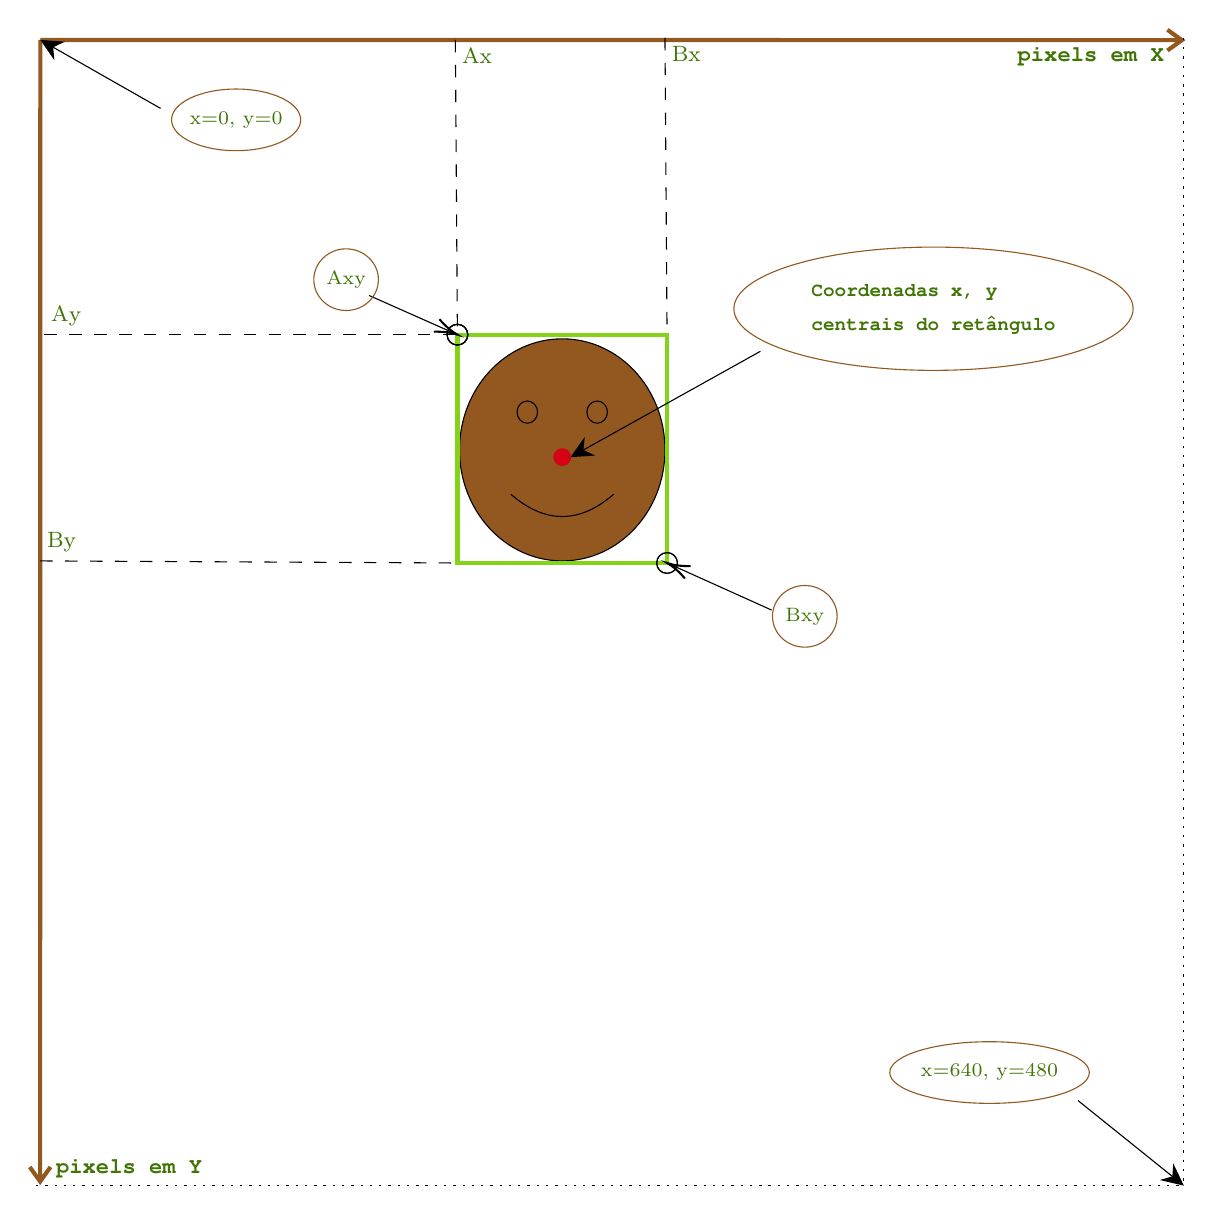
\begin{tikzpicture}[x=0.75pt,y=0.75pt,yscale=-1,xscale=1]
%uncomment if require: \path (0,802); %set diagram left start at 0, and has height of 802

%Shape: Axis 2D [id:dp4555798124742032] 
\draw [color={rgb, 255:red, 139; green, 87; blue, 42 }  ,draw opacity=1 ][line width=1.5]  (69.05,49.5) -- (68.95,599.5)(619.05,49.6) -- (69.05,49.5) -- cycle (73.95,592.5) -- (68.95,599.5) -- (63.95,592.5) (612.05,44.59) -- (619.05,49.6) -- (612.05,54.59)  ;
%Shape: Smiley Face [id:dp9391359153155296] 
\draw  [fill={rgb, 255:red, 139; green, 87; blue, 42 }  ,fill opacity=1 ] (271,247) .. controls (271,217.45) and (293.16,193.5) .. (320.5,193.5) .. controls (347.84,193.5) and (370,217.45) .. (370,247) .. controls (370,276.55) and (347.84,300.5) .. (320.5,300.5) .. controls (293.16,300.5) and (271,276.55) .. (271,247) -- cycle ; \draw  [fill={rgb, 255:red, 139; green, 87; blue, 42 }  ,fill opacity=1 ] (298.72,228.81) .. controls (298.72,225.86) and (300.94,223.46) .. (303.67,223.46) .. controls (306.4,223.46) and (308.62,225.86) .. (308.62,228.81) .. controls (308.62,231.76) and (306.4,234.16) .. (303.67,234.16) .. controls (300.94,234.16) and (298.72,231.76) .. (298.72,228.81) -- cycle ; \draw  [fill={rgb, 255:red, 139; green, 87; blue, 42 }  ,fill opacity=1 ] (332.38,228.81) .. controls (332.38,225.86) and (334.6,223.46) .. (337.33,223.46) .. controls (340.06,223.46) and (342.28,225.86) .. (342.28,228.81) .. controls (342.28,231.76) and (340.06,234.16) .. (337.33,234.16) .. controls (334.6,234.16) and (332.38,231.76) .. (332.38,228.81) -- cycle ; \draw   (295.75,268.4) .. controls (312.25,282.67) and (328.75,282.67) .. (345.25,268.4) ;
%Flowchart: Process [id:dp39379292608490624] 
\draw  [color={rgb, 255:red, 126; green, 211; blue, 33 }  ,draw opacity=1 ][line width=1.5]  (270,191.5) -- (371,191.5) -- (371,301.5) -- (270,301.5) -- cycle ;
%Straight Lines [id:da3834962043936656] 
\draw  [dash pattern={on 0.84pt off 2.51pt}]  (620,48.5) -- (620,601.5) ;
%Straight Lines [id:da28721230743083104] 
\draw  [dash pattern={on 0.84pt off 2.51pt}]  (67,601.5) -- (620,601.5) ;
%Straight Lines [id:da5550623511504473] 
\draw  [dash pattern={on 4.5pt off 4.5pt}]  (69,300.5) -- (270,301.5) ;
%Straight Lines [id:da3939101175382884] 
\draw  [dash pattern={on 4.5pt off 4.5pt}]  (71,191.5) -- (270,191.5) ;
%Straight Lines [id:da2141409001446355] 
\draw  [dash pattern={on 4.5pt off 4.5pt}]  (269,49.5) -- (270,191.5) ;
%Straight Lines [id:da6633828936036013] 
\draw  [dash pattern={on 4.5pt off 4.5pt}]  (370,48.5) -- (371,191.5) ;
%Shape: Circle [id:dp6494670108776119] 
\draw  [color={rgb, 255:red, 208; green, 2; blue, 27 }  ,draw opacity=1 ][fill={rgb, 255:red, 208; green, 2; blue, 27 }  ,fill opacity=1 ] (316.5,250.5) .. controls (316.5,248.29) and (318.29,246.5) .. (320.5,246.5) .. controls (322.71,246.5) and (324.5,248.29) .. (324.5,250.5) .. controls (324.5,252.71) and (322.71,254.5) .. (320.5,254.5) .. controls (318.29,254.5) and (316.5,252.71) .. (316.5,250.5) -- cycle ;
%Straight Lines [id:da15209721546831734] 
\draw    (416,199.5) -- (327.12,249.04) ;
\draw [shift={(324.5,250.5)}, rotate = 330.87] [fill={rgb, 255:red, 0; green, 0; blue, 0 }  ][line width=0.08]  [draw opacity=0] (10.72,-5.15) -- (0,0) -- (10.72,5.15) -- (7.12,0) -- cycle    ;
%Straight Lines [id:da4691908809525298] 
\draw    (127,82.5) -- (71.65,50.98) ;
\draw [shift={(69.05,49.5)}, rotate = 389.65999999999997] [fill={rgb, 255:red, 0; green, 0; blue, 0 }  ][line width=0.08]  [draw opacity=0] (10.72,-5.15) -- (0,0) -- (10.72,5.15) -- (7.12,0) -- cycle    ;
%Straight Lines [id:da8244683672036353] 
\draw    (569,560.5) -- (617.66,599.62) ;
\draw [shift={(620,601.5)}, rotate = 218.8] [fill={rgb, 255:red, 0; green, 0; blue, 0 }  ][line width=0.08]  [draw opacity=0] (10.72,-5.15) -- (0,0) -- (10.72,5.15) -- (7.12,0) -- cycle    ;
%Straight Lines [id:da7964680967109363] 
\draw [color={rgb, 255:red, 0; green, 0; blue, 0 }  ,draw opacity=0 ][fill={rgb, 255:red, 0; green, 0; blue, 0 }  ,fill opacity=0 ]   (371,301.5) -- (371,292.2) ;
%Straight Lines [id:da01751891515099846] 
\draw    (227.4,172.6) -- (268.17,190.69) ;
\draw [shift={(270,191.5)}, rotate = 203.93] [color={rgb, 255:red, 0; green, 0; blue, 0 }  ][line width=0.75]    (10.93,-3.29) .. controls (6.95,-1.4) and (3.31,-0.3) .. (0,0) .. controls (3.31,0.3) and (6.95,1.4) .. (10.93,3.29)   ;
%Straight Lines [id:da05405515080457568] 
\draw    (421.4,324.2) -- (372.82,302.32) ;
\draw [shift={(371,301.5)}, rotate = 384.25] [color={rgb, 255:red, 0; green, 0; blue, 0 }  ][line width=0.75]    (10.93,-3.29) .. controls (6.95,-1.4) and (3.31,-0.3) .. (0,0) .. controls (3.31,0.3) and (6.95,1.4) .. (10.93,3.29)   ;

% Text Node
\draw  [color={rgb, 255:red, 139; green, 87; blue, 42 }  ,draw opacity=1 ]  (526.37, 547) circle [x radius= 48.08, y radius= 14.85]   ;
\draw (526.37,547) node   [align=left] {{\scriptsize \textcolor[rgb]{0.25,0.46,0.02}{{\fontfamily{helvet}\selectfont x=640, y=480}}}};
% Text Node
\draw  [color={rgb, 255:red, 139; green, 87; blue, 42 }  ,draw opacity=1 ]  (437.37, 327.2) circle [x radius= 15.56, y radius= 14.85]   ;
\draw (437.37,327.2) node   [align=left] {{\scriptsize \textcolor[rgb]{0.25,0.46,0.02}{{\fontfamily{helvet}\selectfont Bxy}}}};
% Text Node
\draw  [color={rgb, 255:red, 139; green, 87; blue, 42 }  ,draw opacity=1 ]  (216.37, 165) circle [x radius= 15.56, y radius= 14.85]   ;
\draw (216.37,165) node   [align=left] {{\scriptsize \textcolor[rgb]{0.25,0.46,0.02}{{\fontfamily{helvet}\selectfont Axy}}}};
% Text Node
\draw  [color={rgb, 255:red, 139; green, 87; blue, 42 }  ,draw opacity=1 ]  (163.37, 88) circle [x radius= 31.11, y radius= 14.85]   ;
\draw (163.37,88) node   [align=left] {{\scriptsize \textcolor[rgb]{0.25,0.46,0.02}{{\fontfamily{helvet}\selectfont x=0, y=0}}}};
% Text Node
\draw  [color={rgb, 255:red, 139; green, 87; blue, 42 }  ,draw opacity=1 ]  (499.37, 179) circle [x radius= 96.17, y radius= 29.7]   ;
\draw (499.37,179) node   [align=left] {{\scriptsize \textcolor[rgb]{0.25,0.46,0.02}{\textbf{{\fontfamily{pcr}\selectfont Coordenadas x, y}}}}\\{\scriptsize \textcolor[rgb]{0.25,0.46,0.02}{\textbf{{\fontfamily{pcr}\selectfont centrais do retângulo}}}}};
% Text Node
\draw (69,598.5) node [anchor=south west] [inner sep=0.75pt]   [align=left] {{\footnotesize \textbf{\textcolor[rgb]{0.25,0.46,0.02}{{\fontfamily{pcr}\selectfont  \ pixels em Y}}}}};
% Text Node
\draw (618,51.5) node [anchor=north east] [inner sep=0.75pt]   [align=left] {{\footnotesize \textbf{\textcolor[rgb]{0.25,0.46,0.02}{{\fontfamily{pcr}\selectfont pixels em X }}}}};
% Text Node
\draw (271,52.5) node [anchor=north west][inner sep=0.75pt]   [align=left] {{\fontfamily{helvet}\selectfont {\footnotesize \textcolor[rgb]{0.25,0.46,0.02}{Ax}}}};
% Text Node
\draw (73,188.5) node [anchor=south west] [inner sep=0.75pt]   [align=left] {{\fontfamily{helvet}\selectfont {\footnotesize \textcolor[rgb]{0.25,0.46,0.02}{Ay}}}};
% Text Node
\draw (71,297.5) node [anchor=south west] [inner sep=0.75pt]   [align=left] {{\fontfamily{helvet}\selectfont {\footnotesize \textcolor[rgb]{0.25,0.46,0.02}{By}}}};
% Text Node
\draw (372,51.5) node [anchor=north west][inner sep=0.75pt]   [align=left] {{\fontfamily{helvet}\selectfont {\footnotesize \textcolor[rgb]{0.25,0.46,0.02}{Bx}}}};

\draw   (270, 191.5) circle [x radius= 5, y radius= 5]   ;
\draw   (270, 191.5) circle [x radius= 5, y radius= 5]   ;
\draw   (270, 191.5) circle [x radius= 5, y radius= 5]   ;
\draw   (371, 301.5) circle [x radius= 5, y radius= 5]   ;
\draw   (371, 301.5) circle [x radius= 5, y radius= 5]   ;
\end{tikzpicture}

	\legend{Fonte: do autor}
	\label{fig:quad1}
\end{figure}

Para que o sistema funciona-se as coordenadas X=0 e Y=0 foram transportadas para um ponto central da tela, portanto foram realizados cálculos para determinar dois eixos um na horizontal e outro na vertical e sua intersecção ou ponto médio é o epicentro do novo sistema de coordenadas. Na ilustração \ref{fig:quad2} as duas retas na cor marrom representam o novo sistema, assim foi possível equacionar um novo ponto central para o retângulo que é  desenhado em torno da face, esse novo ponto é dado como B' e ele recebe os valores calculados para fx' e fy'.   

\begin{figure}[H]
	\centering
	\caption{Conversão do Sistema de Coordenadas OpenCV para Coordenadas Cartesianas}
		\tikzset{every picture/.style={line width=0.75pt}} %set default line width to 0.75pt        
	
	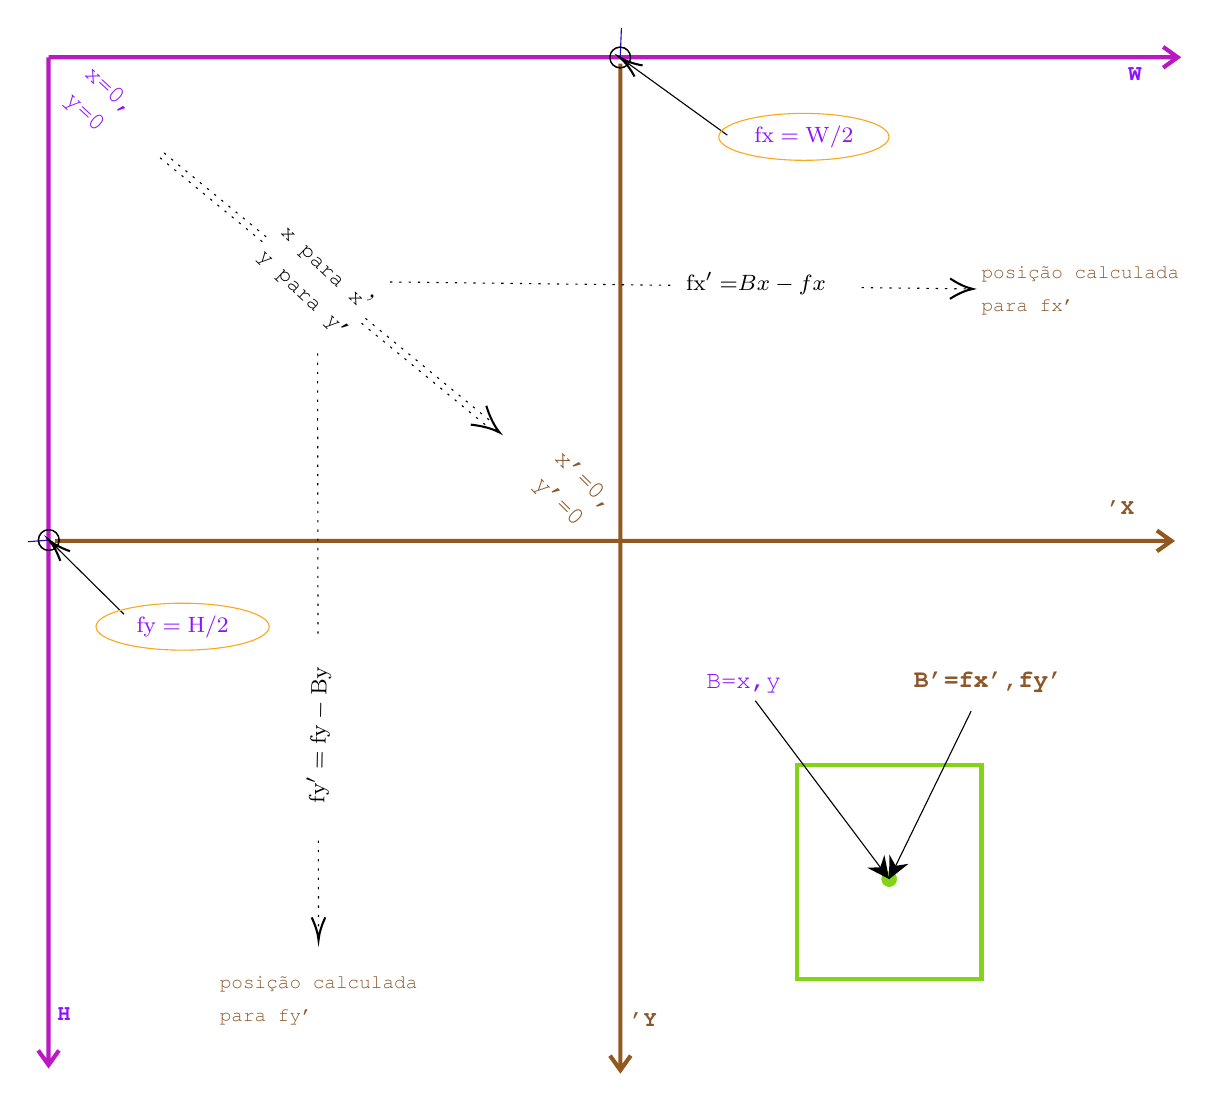
\begin{tikzpicture}[x=0.75pt,y=0.75pt,yscale=-1,xscale=1]
	%uncomment if require: \path (0,578); %set diagram left start at 0, and has height of 578
	
	%Shape: Axis 2D [id:dp745366717574464] 
	\draw [color={rgb, 255:red, 139; green, 87; blue, 42 }  ,draw opacity=1 ][line width=1.5]  (305.5,41) -- (305.5,526)(571,271) -- (33,271) (310.5,519) -- (305.5,526) -- (300.5,519) (564,266) -- (571,271) -- (564,276)  ;
	%Shape: Rectangle [id:dp835814910936395] 
	\draw  [color={rgb, 255:red, 126; green, 211; blue, 33 }  ,draw opacity=1 ][line width=1.5]  (390.5,482) -- (390.5,378.9) -- (479.5,378.9) -- (479.5,482) -- cycle ;
	%Shape: Circle [id:dp6195483350711979] 
	\draw  [color={rgb, 255:red, 126; green, 211; blue, 33 }  ,draw opacity=1 ][fill={rgb, 255:red, 126; green, 211; blue, 33 }  ,fill opacity=1 ] (431.5,433.95) .. controls (431.5,432.02) and (433.07,430.45) .. (435,430.45) .. controls (436.93,430.45) and (438.5,432.02) .. (438.5,433.95) .. controls (438.5,435.88) and (436.93,437.45) .. (435,437.45) .. controls (433.07,437.45) and (431.5,435.88) .. (431.5,433.95) -- cycle ;
	%Shape: Axis 2D [id:dp10273922885069342] 
	\draw [color={rgb, 255:red, 144; green, 19; blue, 254 }  ,draw opacity=1 ][line width=1.5]  (30,38) -- (30,523.5)(574,38) -- (30,38) -- cycle (35,516.5) -- (30,523.5) -- (25,516.5) (567,33) -- (574,38) -- (567,43)  ;
	%Straight Lines [id:da39018414566648474] 
	\draw    (370.5,348) -- (433.2,431.55) ;
	\draw [shift={(435,433.95)}, rotate = 233.11] [fill={rgb, 255:red, 0; green, 0; blue, 0 }  ][line width=0.08]  [draw opacity=0] (10.72,-5.15) -- (0,0) -- (10.72,5.15) -- (7.12,0) -- cycle    ;
	%Straight Lines [id:da811434966043961] 
	\draw    (474.5,353) -- (454.7,393.58) -- (436.32,431.25) ;
	\draw [shift={(435,433.95)}, rotate = 296.01] [fill={rgb, 255:red, 0; green, 0; blue, 0 }  ][line width=0.08]  [draw opacity=0] (10.72,-5.15) -- (0,0) -- (10.72,5.15) -- (7.12,0) -- cycle    ;
	%Straight Lines [id:da7444934143033615] 
	\draw [color={rgb, 255:red, 255; green, 255; blue, 255 }  ,draw opacity=1 ]   (306,24) -- (305.4,38.2) ;
	%Straight Lines [id:da5396729355438599] 
	\draw [color={rgb, 255:red, 255; green, 255; blue, 255 }  ,draw opacity=1 ]   (20.2,271.4) -- (30.2,270.6) ;
	%Straight Lines [id:da7044410949948923] 
	\draw    (357,75.5) -- (307.02,39.37) ;
	\draw [shift={(305.4,38.2)}, rotate = 395.86] [color={rgb, 255:red, 0; green, 0; blue, 0 }  ][line width=0.75]    (10.93,-3.29) .. controls (6.95,-1.4) and (3.31,-0.3) .. (0,0) .. controls (3.31,0.3) and (6.95,1.4) .. (10.93,3.29)   ;
	%Straight Lines [id:da8627654662164674] 
	\draw    (66.33,306.33) -- (31.62,272.01) ;
	\draw [shift={(30.2,270.6)}, rotate = 404.68] [color={rgb, 255:red, 0; green, 0; blue, 0 }  ][line width=0.75]    (10.93,-3.29) .. controls (6.95,-1.4) and (3.31,-0.3) .. (0,0) .. controls (3.31,0.3) and (6.95,1.4) .. (10.93,3.29)   ;
	
	% Text Node
	\draw (539,251) node [anchor=north west][inner sep=0.75pt]   [align=left] {{\fontfamily{pcr}\selectfont {\footnotesize \textbf{\textcolor[rgb]{0.55,0.34,0.16}{'X}}}}};
	% Text Node
	\draw (309,498) node [anchor=north west][inner sep=0.75pt]   [align=left] {{\fontfamily{pcr}\selectfont {\footnotesize \textbf{\textcolor[rgb]{0.55,0.34,0.16}{'Y}}}}};
	% Text Node
	\draw (549,42) node [anchor=north west][inner sep=0.75pt]   [align=left] {{\fontfamily{pcr}\selectfont {\footnotesize \textbf{\textcolor[rgb]{0.56,0.07,1}{W}}}}};
	% Text Node
	\draw (33,495) node [anchor=north west][inner sep=0.75pt]   [align=left] {{\fontfamily{pcr}\selectfont {\footnotesize \textbf{\textcolor[rgb]{0.56,0.07,1}{H}}}}};
	% Text Node
	\draw (364.91,339.5) node   [align=left] {{\fontfamily{pcr}\selectfont {\small \textcolor[rgb]{0.56,0.07,1}{B=x,y}}}};
	% Text Node
	\draw (31.47,39.36) node [anchor=west] [inner sep=0.75pt]  [rotate=-42.7] [align=left] {\begin{minipage}[lt]{41.469392000000006pt}\setlength\topsep{0pt}
		\begin{center}
		{\fontfamily{pcr}\selectfont {\small \textcolor[rgb]{0.56,0.07,1}{x=0, y=0}}}
		\end{center}
		
		\end{minipage}};
	% Text Node
	\draw (304.09,269.59) node [anchor=east] [inner sep=0.75pt]  [rotate=-45] [align=left] {\begin{minipage}[lt]{46.569392pt}\setlength\topsep{0pt}
		\begin{center}
		{\fontfamily{pcr}\selectfont {\small \textcolor[rgb]{0.55,0.34,0.16}{x'=0, y'=0}}}
		\end{center}
		
		\end{minipage}};
	% Text Node
	\draw (159.54,145.82) node  [rotate=-43.61] [align=left] {{\fontfamily{pcr}\selectfont {\footnotesize x para x}}'\\{\footnotesize {\fontfamily{pcr}\selectfont y para y'}}};
	% Text Node
	\draw (478.27,150.17) node [anchor=west] [inner sep=0.75pt]   [align=left] {{\fontfamily{pcr}\selectfont {\scriptsize \textcolor[rgb]{0.55,0.34,0.16}{posição calculada}}}\\{\fontfamily{pcr}\selectfont {\scriptsize \textcolor[rgb]{0.55,0.34,0.16}{ para fx' }}}};
	% Text Node
	\draw (160.1,505.33) node [anchor=south] [inner sep=0.75pt]   [align=left] {{\fontfamily{pcr}\selectfont {\scriptsize \textcolor[rgb]{0.55,0.34,0.16}{posição calculada}}}\\{\fontfamily{pcr}\selectfont {\scriptsize \textcolor[rgb]{0.55,0.34,0.16}{ para fy'}}}};
	% Text Node
	\draw (482.91,338.5) node   [align=left] {\textbf{{\fontfamily{pcr}\selectfont {\small \textcolor[rgb]{0.55,0.34,0.16}{B'=fx',fy'}}}}};
	% Text Node
	\draw (370.81,147) node  [font=\footnotesize]  {${\displaystyle \mathrm{fx'=} Bx-fx}$};
	% Text Node
	\draw  [color={rgb, 255:red, 245; green, 166; blue, 35 }  ,draw opacity=1 ]  (94.58, 312.33) circle [x radius= 41.72, y radius= 11.31]   ;
	\draw (94.58,312.33) node  [font=\footnotesize]  {${\displaystyle \mathrm{\textcolor[rgb]{0.56,0.07,1}{fy=H/2}}}$};
	% Text Node
	\draw  [color={rgb, 255:red, 245; green, 166; blue, 35 }  ,draw opacity=1 ]  (393.91, 76.33) circle [x radius= 41.01, y radius= 11.31]   ;
	\draw (393.91,76.33) node  [font=\footnotesize]  {${\displaystyle \mathrm{\textcolor[rgb]{0.56,0.07,1}{fx=W/2}}}$};
	% Text Node
	\draw (160.14,364.33) node  [font=\footnotesize,rotate=-271.05]  {$\mathrm{{\displaystyle fy'=fy-By}}$};
	% Connection
	\draw  [dash pattern={on 0.84pt off 2.51pt}]  (85.64,84.1) -- (136.33,125.72)(182.7,163.8) -- (242.83,213.17)(83.73,86.42) -- (134.42,128.04)(180.79,166.12) -- (240.92,215.49) ;
	\draw [shift={(247.29,218.77)}, rotate = 219.39] [color={rgb, 255:red, 0; green, 0; blue, 0 }  ][line width=0.75]    (13.12,-5.88) .. controls (8.34,-2.76) and (3.97,-0.8) .. (0,0) .. controls (3.97,0.8) and (8.34,2.76) .. (13.12,5.88)   ;
	% Connection
	\draw  [dash pattern={on 0.84pt off 2.51pt}]  (194.49,146.24) -- (329.7,147.86)(421.69,148.97) -- (473.27,149.58) ;
	\draw [shift={(475.27,149.61)}, rotate = 180.69] [color={rgb, 255:red, 0; green, 0; blue, 0 }  ][line width=0.75]    (10.93,-4.9) .. controls (6.95,-2.3) and (3.31,-0.67) .. (0,0) .. controls (3.31,0.67) and (6.95,2.3) .. (10.93,4.9)   ;
	% Connection
	\draw  [dash pattern={on 0.84pt off 2.51pt}]  (159.6,180.61) -- (159.82,316.39)(159.99,415.39) -- (160.06,461.33) ;
	\draw [shift={(160.07,463.33)}, rotate = 269.90999999999997] [color={rgb, 255:red, 0; green, 0; blue, 0 }  ][line width=0.75]    (10.93,-3.29) .. controls (6.95,-1.4) and (3.31,-0.3) .. (0,0) .. controls (3.31,0.3) and (6.95,1.4) .. (10.93,3.29)   ;
	\draw   (30, 270.62) circle [x radius= 5, y radius= 5]   ;
	\draw   (30.2, 270.6) circle [x radius= 5, y radius= 5]   ;
	\draw   (305.41, 38) circle [x radius= 5, y radius= 5]   ;
	\draw   (305.4, 38.2) circle [x radius= 5, y radius= 5]   ;
	\end{tikzpicture}

	\legend{Fonte: do autor}
	\label{fig:quad2}
\end{figure}

O objetivo de obter um sistema de coordenadas que pudesse ser utilizado para orientar o direcionamento do VANT foi alcançado e ele pode ser observado na ilustração \ref{fig:teste}, esse sistema de coordenadas é denominado de cartesiano e possui quatro quadrantes distintos e bem definidos, é o mesmo utilizado para localização geográfica na superfície terrestre. Da mesmo forma que aeronaves conseguem se orientar na superfície terrestre usando coordenadas cartesianas, também é possível guiar um VANT para chegar ao objetivo do protótipo.

Com o novo sistema de coordenadas foi possivel obter valores para X e Y com uma maior precisão (0.005m/s a 5m/s), assim como os quatro quadrantes conseguem indicar para qual direção a aeronave tem que se deslocar. Esses valores de velocidade posteriormente serão enviados para a controladora de voo do VANT. 

A interpretação das informações da ilustração \ref{fig:quad2} pode ser feita através das seguintes sintaxes matemáticas; 

\begin{itemize}
	\item Sintaxe do quadrante I:\begin{equation}\label{q1} B'\in (Quadrante\ I) \mid \left(Bx - \frac{W}{2} >0\right) \land \left(\frac{H}{2} - By >0\right)\end{equation} 
	\item Sintaxe do quadrante II:\begin{equation}\label{q2} B'\in (Quadrante\ II) \mid \left(Bx - \frac{W}{2} <0\right) \land \left(\frac{H}{2} - By >0\right)\end{equation} 
	\item Sintaxe do quadrante III:\begin{equation}\label{q3} B'\in (Quadrante\ III) \mid \left(Bx - \frac{W}{2} <0\right) \land \left(\frac{H}{2} - By <0\right)\end{equation} 
	\item Sintaxe do quadrante IV:\begin{equation}\label{q4} B'\in (Quadrante\ IV) \mid \left(Bx - \frac{W}{2} >0\right) \land \left(\frac{H}{2} - By <0\right)\end{equation} 
	\item Sintaxe quando não pertence a nenhum quadrante:\begin{equation}\label{nq} B'\notin ( Quadrante\ I\lor II\lor III\lor IV) \mid \left(Bx - \frac{W}{2}=0\right) \lor \left(\frac{H}{2} - By =0\right)\end{equation}
\end{itemize} 

\begin{figure}[H]
	\centering
	\caption{Sistema de Coordenadas Cartesianas em Visão Computacional}
		\tikzset{every picture/.style={line width=0.75pt}} %set default line width to 0.75pt        
	
	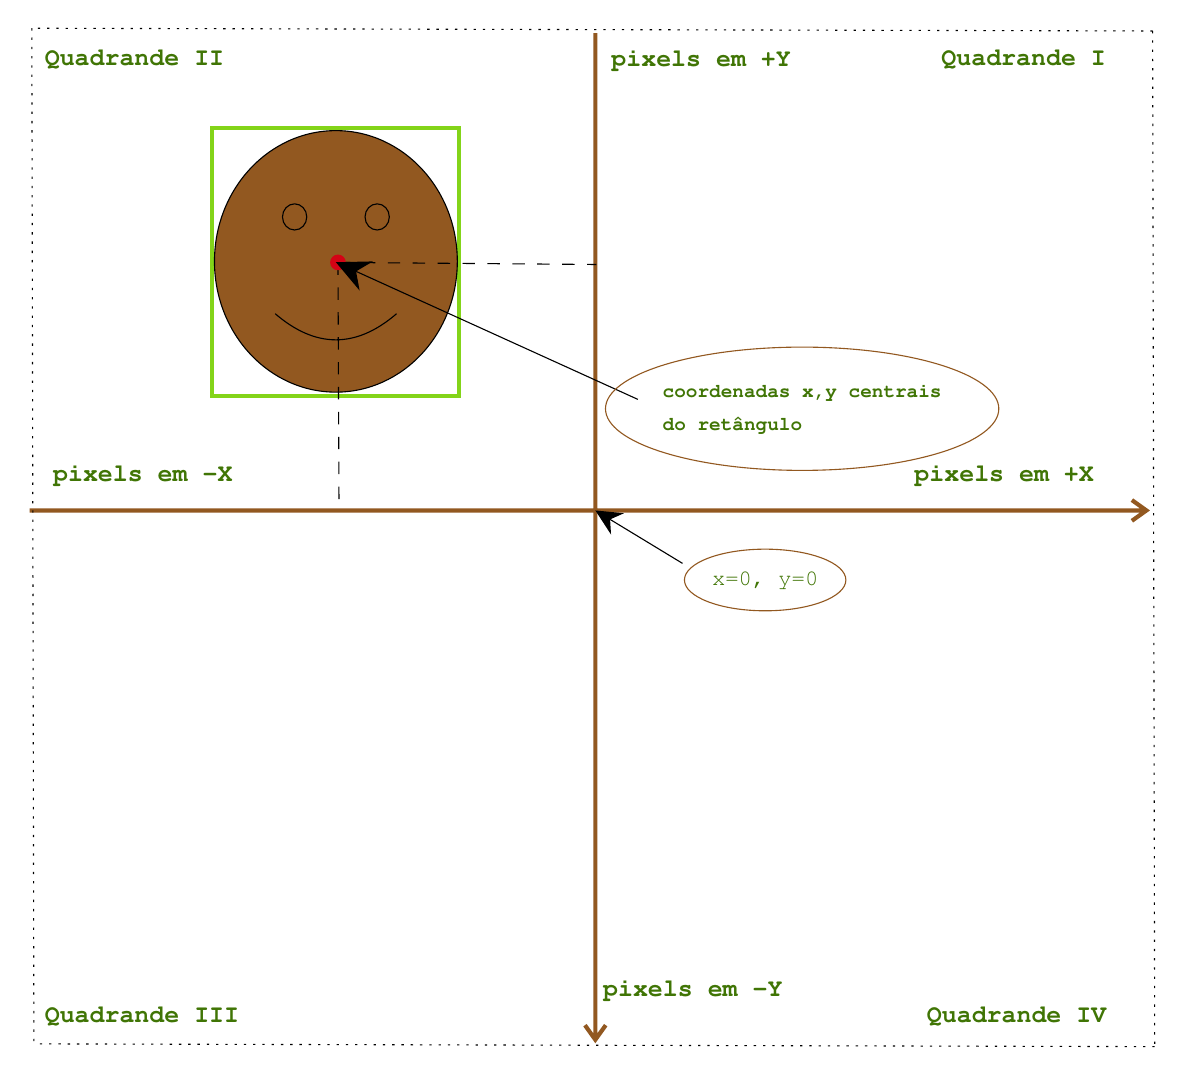
\begin{tikzpicture}[x=0.75pt,y=0.75pt,yscale=-1,xscale=1]
	%uncomment if require: \path (0,578); %set diagram left start at 0, and has height of 578
	
	%Shape: Axis 2D [id:dp745366717574464] 
	\draw [color={rgb, 255:red, 139; green, 87; blue, 42 }  ,draw opacity=1 ][line width=1.5]  (281.5,12) -- (281.5,497)(547,242) -- (9,242) (286.5,490) -- (281.5,497) -- (276.5,490) (540,237) -- (547,242) -- (540,247)  ;
	%Shape: Rectangle [id:dp835814910936395] 
	\draw  [color={rgb, 255:red, 126; green, 211; blue, 33 }  ,draw opacity=1 ][line width=1.5]  (97,187) -- (97,57.8) -- (216,57.8) -- (216,187) -- cycle ;
	%Shape: Smiley Face [id:dp00370584545415098] 
	\draw  [fill={rgb, 255:red, 139; green, 87; blue, 42 }  ,fill opacity=1 ] (98,122) .. controls (98,87.21) and (124.19,59) .. (156.5,59) .. controls (188.81,59) and (215,87.21) .. (215,122) .. controls (215,156.79) and (188.81,185) .. (156.5,185) .. controls (124.19,185) and (98,156.79) .. (98,122) -- cycle ; \draw  [fill={rgb, 255:red, 139; green, 87; blue, 42 }  ,fill opacity=1 ] (130.76,100.58) .. controls (130.76,97.1) and (133.38,94.28) .. (136.61,94.28) .. controls (139.84,94.28) and (142.46,97.1) .. (142.46,100.58) .. controls (142.46,104.06) and (139.84,106.88) .. (136.61,106.88) .. controls (133.38,106.88) and (130.76,104.06) .. (130.76,100.58) -- cycle ; \draw  [fill={rgb, 255:red, 139; green, 87; blue, 42 }  ,fill opacity=1 ] (170.54,100.58) .. controls (170.54,97.1) and (173.16,94.28) .. (176.39,94.28) .. controls (179.62,94.28) and (182.24,97.1) .. (182.24,100.58) .. controls (182.24,104.06) and (179.62,106.88) .. (176.39,106.88) .. controls (173.16,106.88) and (170.54,104.06) .. (170.54,100.58) -- cycle ; \draw   (127.25,147.2) .. controls (146.75,164) and (166.25,164) .. (185.75,147.2) ;
	%Straight Lines [id:da45515329684866135] 
	\draw [color={rgb, 255:red, 0; green, 0; blue, 0 }  ,draw opacity=1 ] [dash pattern={on 0.84pt off 2.51pt}]  (550,11) -- (551,500.33) ;
	%Straight Lines [id:da24415373962833065] 
	\draw [color={rgb, 255:red, 0; green, 0; blue, 0 }  ,draw opacity=1 ] [dash pattern={on 0.84pt off 2.51pt}]  (551,500.33) -- (11,499) ;
	%Straight Lines [id:da6205263233417599] 
	\draw  [dash pattern={on 4.5pt off 4.5pt}]  (157.5,122.5) -- (282,123.5) ;
	%Straight Lines [id:da2467412144940746] 
	\draw  [dash pattern={on 4.5pt off 4.5pt}]  (157.5,122.5) -- (158,241.5) ;
	%Shape: Circle [id:dp6195483350711979] 
	\draw  [color={rgb, 255:red, 208; green, 2; blue, 27 }  ,draw opacity=1 ][fill={rgb, 255:red, 208; green, 2; blue, 27 }  ,fill opacity=1 ] (154,122.5) .. controls (154,120.57) and (155.57,119) .. (157.5,119) .. controls (159.43,119) and (161,120.57) .. (161,122.5) .. controls (161,124.43) and (159.43,126) .. (157.5,126) .. controls (155.57,126) and (154,124.43) .. (154,122.5) -- cycle ;
	%Straight Lines [id:da3852329060686428] 
	\draw    (302,188.5) -- (159.23,123.64) ;
	\draw [shift={(156.5,122.4)}, rotate = 384.43] [fill={rgb, 255:red, 0; green, 0; blue, 0 }  ][line width=0.08]  [draw opacity=0] (16.07,-7.72) -- (0,0) -- (16.07,7.72) -- (10.67,0) -- cycle    ;
	%Straight Lines [id:da7942156802276659] 
	\draw    (323.5,267.5) -- (284.06,243.56) ;
	\draw [shift={(281.5,242)}, rotate = 391.26] [fill={rgb, 255:red, 0; green, 0; blue, 0 }  ][line width=0.08]  [draw opacity=0] (12.5,-6.01) -- (0,0) -- (12.5,6.01) -- (8.3,0) -- cycle    ;
	%Straight Lines [id:da8593503836199177] 
	\draw [color={rgb, 255:red, 0; green, 0; blue, 0 }  ,draw opacity=1 ] [dash pattern={on 0.84pt off 2.51pt}]  (10,9.67) -- (11,499) ;
	%Straight Lines [id:da5989886602637362] 
	\draw [color={rgb, 255:red, 0; green, 0; blue, 0 }  ,draw opacity=1 ] [dash pattern={on 0.84pt off 2.51pt}]  (550,11) -- (10,9.67) ;
	
	% Text Node
	\draw (434,219) node [anchor=north west][inner sep=0.75pt]   [align=left] {{\fontfamily{pcr}\selectfont {\small \textbf{\textcolor[rgb]{0.25,0.46,0.02}{pixels em +X}}}}};
	% Text Node
	\draw (284,467) node [anchor=north west][inner sep=0.75pt]   [align=left] {{\fontfamily{pcr}\selectfont {\small \textbf{\textcolor[rgb]{0.25,0.46,0.02}{pixels em -Y}}}}};
	% Text Node
	\draw  [color={rgb, 255:red, 139; green, 87; blue, 42 }  ,draw opacity=1 ]  (363.32, 275.5) circle [x radius= 38.89, y radius= 14.85]   ;
	\draw (363.32,275.5) node   [align=left] {{\fontfamily{pcr}\selectfont {\footnotesize \textcolor[rgb]{0.25,0.46,0.02}{x=0, y=0}}}};
	% Text Node
	\draw  [color={rgb, 255:red, 139; green, 87; blue, 42 }  ,draw opacity=1 ]  (381.14, 193) circle [x radius= 94.75, y radius= 29.7]   ;
	\draw (381.14,193) node   [align=left] {{\fontfamily{pcr}\selectfont {\scriptsize \textbf{\textcolor[rgb]{0.25,0.46,0.02}{coordenadas x,y centrais}}}}\\{\fontfamily{pcr}\selectfont {\scriptsize \textbf{\textcolor[rgb]{0.25,0.46,0.02}{ do retângulo}}}}};
	% Text Node
	
	\draw (447,19) node [anchor=north west][inner sep=0.75pt]   [align=left] {{\fontfamily{pcr}\selectfont {\small \textbf{\textcolor[rgb]{0.25,0.46,0.02}{Quadrande I}}}}};
	
	\draw (15,19) node [anchor=north west][inner sep=0.75pt]   [align=left] {{\fontfamily{pcr}\selectfont {\small \textbf{\textcolor[rgb]{0.25,0.46,0.02}{Quadrande II}}}}};
	
	\draw (15,480) node [anchor=north west][inner sep=0.75pt]   [align=left] {{\fontfamily{pcr}\selectfont {\small \textbf{\textcolor[rgb]{0.25,0.46,0.02}{Quadrande III}}}}};
	
	\draw (440,480) node [anchor=north west][inner sep=0.75pt]   [align=left] {{\fontfamily{pcr}\selectfont {\small \textbf{\textcolor[rgb]{0.25,0.46,0.02}{Quadrande IV}}}}};
	
	\draw (288,19) node [anchor=north west][inner sep=0.75pt]   [align=left] {{\fontfamily{pcr}\selectfont {\small \textbf{\textcolor[rgb]{0.25,0.46,0.02}{pixels em +Y}}}}};
	% Text Node
	\draw (19,219) node [anchor=north west][inner sep=0.75pt]   [align=left] {{\fontfamily{pcr}\selectfont {\small \textbf{\textcolor[rgb]{0.25,0.46,0.02}{pixels em -X}}}}};
	
	
	\end{tikzpicture}

	\legend{Fonte: do autor}
	\label{fig:teste}
\end{figure}

Para concluir essa parte a ilustração \ref{fig:conv} representa a projeção em 3D do sistema de coordenadas original que o OpenCV utiliza e como fica apos a transformação. O OpenCV possui o eixo Z (profundidade), ele é utilizado para calcular a posição em um sistema 3D ou adquirir a velocidade de deslocamento, porem essa etapa não sera abordada mas pode ser um bom tema para trabalhos futuros ou aperfeiçoamento do sistema.

\begin{figure}[H]
	\centering
	\caption{Projeção do Sistema de Coordenadas OpenCV para Cartesianas}
	\tikzset{every picture/.style={line width=0.75pt}} %set default line width to 0.75pt        

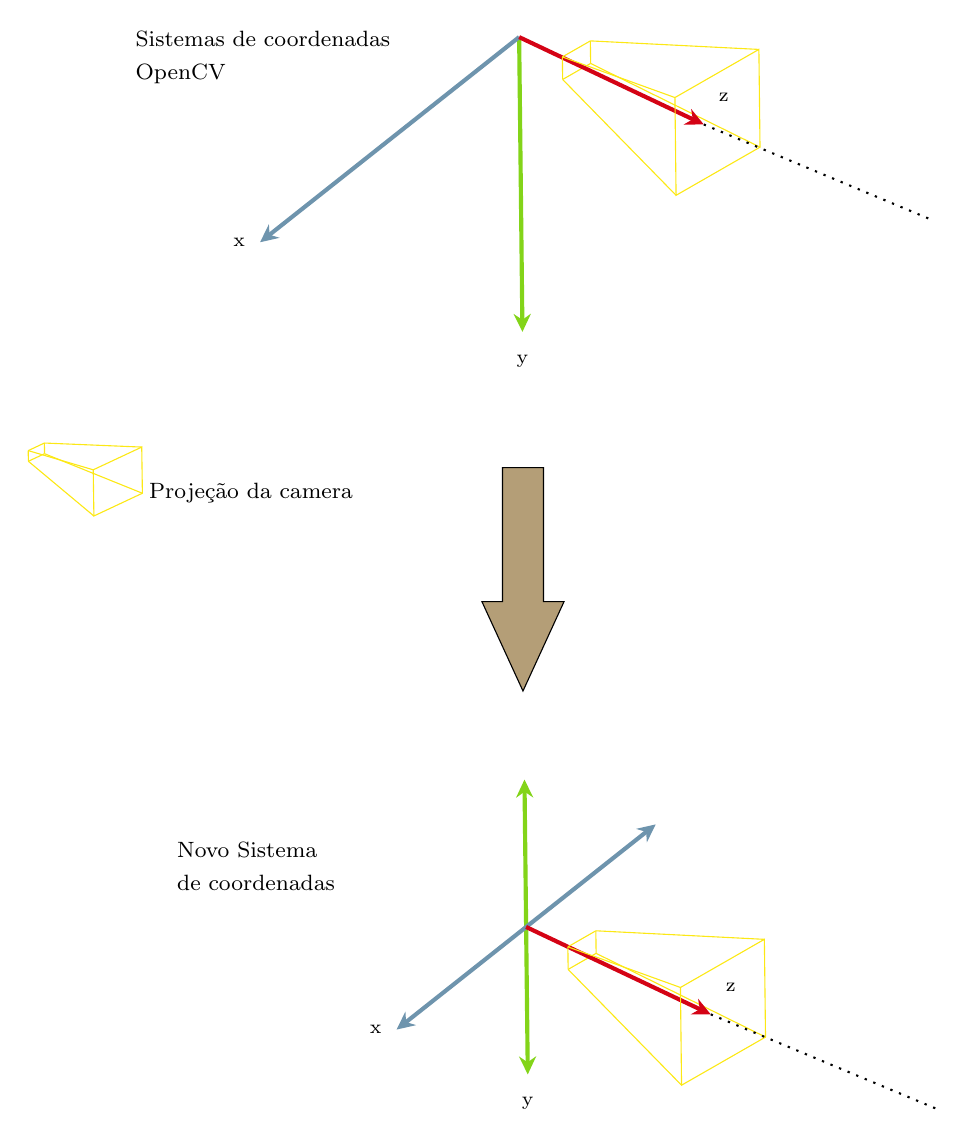
\begin{tikzpicture}[x=0.75pt,y=0.75pt,yscale=-1,xscale=1]
%uncomment if require: \path (0,727); %set diagram left start at 0, and has height of 727

%Straight Lines [id:da8001615144062313] 
\draw [color={rgb, 255:red, 248; green, 231; blue, 28 }  ,draw opacity=1 ]   (349.1,534.72) -- (430.72,575.06) ;
%Straight Lines [id:da8329818260451711] 
\draw [color={rgb, 255:red, 248; green, 231; blue, 28 }  ,draw opacity=1 ]   (335.62,542.45) -- (349.1,534.72) ;
%Straight Lines [id:da7695556715638925] 
\draw [color={rgb, 255:red, 248; green, 231; blue, 28 }  ,draw opacity=1 ]   (348.98,523.85) -- (430.18,527.97) ;
%Straight Lines [id:da9044543466107802] 
\draw [color={rgb, 255:red, 248; green, 231; blue, 28 }  ,draw opacity=1 ]   (335.62,542.45) -- (390.27,598.25) ;
%Straight Lines [id:da22005356609354787] 
\draw [color={rgb, 255:red, 248; green, 231; blue, 28 }  ,draw opacity=1 ]   (349.1,534.72) -- (348.98,523.85) ;
%Straight Lines [id:da9896626633232619] 
\draw [color={rgb, 255:red, 248; green, 231; blue, 28 }  ,draw opacity=1 ]   (346.46,105.96) -- (428.07,146.3) ;
%Straight Lines [id:da5692410863526645] 
\draw [color={rgb, 255:red, 248; green, 231; blue, 28 }  ,draw opacity=1 ]   (332.98,113.69) -- (346.46,105.96) ;
%Straight Lines [id:da5136026067630395] 
\draw [color={rgb, 255:red, 248; green, 231; blue, 28 }  ,draw opacity=1 ]   (346.34,95.1) -- (427.53,99.21) ;
%Straight Lines [id:da17262032579023612] 
\draw [color={rgb, 255:red, 248; green, 231; blue, 28 }  ,draw opacity=1 ]   (332.98,113.69) -- (387.62,169.49) ;
%Straight Lines [id:da23592836557912134] 
\draw [color={rgb, 255:red, 248; green, 231; blue, 28 }  ,draw opacity=1 ]   (346.46,105.96) -- (346.34,95.1) ;
%Straight Lines [id:da03483010490843186] 
\draw [color={rgb, 255:red, 126; green, 211; blue, 33 }  ,draw opacity=1 ][line width=1.5]    (312.02,93.27) -- (313.57,231.3) ;
\draw [shift={(313.61,235.3)}, rotate = 269.36] [fill={rgb, 255:red, 126; green, 211; blue, 33 }  ,fill opacity=1 ][line width=0.08]  [draw opacity=0] (8.75,-4.2) -- (0,0) -- (8.75,4.2) -- (5.81,0) -- cycle    ;
%Straight Lines [id:da9692381380892441] 
\draw [color={rgb, 255:red, 74; green, 144; blue, 226 }  ,draw opacity=1 ][line width=1.5]    (312.02,93.27) -- (190.35,189.62) ;
\draw [shift={(187.21,192.11)}, rotate = 321.62] [fill={rgb, 255:red, 74; green, 144; blue, 226 }  ,fill opacity=1 ][line width=0.08]  [draw opacity=0] (8.75,-4.2) -- (0,0) -- (8.75,4.2) -- (5.81,0) -- cycle    ;
%Straight Lines [id:da5157446213760508] 
\draw [line width=0.75]  [dash pattern={on 0.84pt off 2.51pt}]  (400.96,135.36) -- (509.63,180.81) ;
%Straight Lines [id:da8857765937470132] 
\draw [color={rgb, 255:red, 126; green, 211; blue, 33 }  ,draw opacity=1 ][line width=1.5]    (314.63,455.01) -- (316.14,589.03) ;
\draw [shift={(316.18,593.03)}, rotate = 269.36] [fill={rgb, 255:red, 126; green, 211; blue, 33 }  ,fill opacity=1 ][line width=0.08]  [draw opacity=0] (8.75,-4.2) -- (0,0) -- (8.75,4.2) -- (5.81,0) -- cycle    ;
\draw [shift={(314.59,451.01)}, rotate = 89.36] [fill={rgb, 255:red, 126; green, 211; blue, 33 }  ,fill opacity=1 ][line width=0.08]  [draw opacity=0] (8.75,-4.2) -- (0,0) -- (8.75,4.2) -- (5.81,0) -- cycle    ;
%Straight Lines [id:da27683879440028236] 
\draw [color={rgb, 255:red, 74; green, 144; blue, 226 }  ,draw opacity=1 ][line width=1.5]    (374.65,475.09) -- (256.12,568.96) ;
\draw [shift={(252.98,571.44)}, rotate = 321.62] [fill={rgb, 255:red, 74; green, 144; blue, 226 }  ,fill opacity=1 ][line width=0.08]  [draw opacity=0] (8.75,-4.2) -- (0,0) -- (8.75,4.2) -- (5.81,0) -- cycle    ;
\draw [shift={(377.79,472.6)}, rotate = 141.62] [fill={rgb, 255:red, 74; green, 144; blue, 226 }  ,fill opacity=1 ][line width=0.08]  [draw opacity=0] (8.75,-4.2) -- (0,0) -- (8.75,4.2) -- (5.81,0) -- cycle    ;
%Straight Lines [id:da5586532555155173] 
\draw [color={rgb, 255:red, 208; green, 2; blue, 27 }  ,draw opacity=1 ][line width=1.5]    (315.38,522.02) -- (400.71,562.4) ;
\draw [shift={(404.33,564.11)}, rotate = 205.32999999999998] [fill={rgb, 255:red, 208; green, 2; blue, 27 }  ,fill opacity=1 ][line width=0.08]  [draw opacity=0] (8.75,-4.2) -- (0,0) -- (8.75,4.2) -- (5.81,0) -- cycle    ;
%Straight Lines [id:da3266516450132422] 
\draw [color={rgb, 255:red, 208; green, 2; blue, 27 }  ,draw opacity=1 ][line width=1.5]    (312.02,93.27) -- (397.35,133.65) ;
\draw [shift={(400.96,135.36)}, rotate = 205.32999999999998] [fill={rgb, 255:red, 208; green, 2; blue, 27 }  ,fill opacity=1 ][line width=0.08]  [draw opacity=0] (8.75,-4.2) -- (0,0) -- (8.75,4.2) -- (5.81,0) -- cycle    ;
%Straight Lines [id:da22720526471476132] 
\draw [color={rgb, 255:red, 248; green, 231; blue, 28 }  ,draw opacity=1 ]   (332.98,113.69) -- (332.85,102.82) ;
%Straight Lines [id:da7151365124854405] 
\draw [color={rgb, 255:red, 248; green, 231; blue, 28 }  ,draw opacity=1 ]   (332.85,102.82) -- (346.34,95.1) ;
%Flowchart: Process [id:dp5603704463228976] 
\draw  [color={rgb, 255:red, 248; green, 231; blue, 28 }  ,draw opacity=1 ] (387.08,122.4) -- (427.53,99.21) -- (428.07,146.3) -- (387.63,169.5) -- cycle ;
%Straight Lines [id:da449662482122841] 
\draw [color={rgb, 255:red, 248; green, 231; blue, 28 }  ,draw opacity=1 ]   (332.85,102.82) -- (387.08,122.4) ;
%Flowchart: Process [id:dp31955381373585023] 
\draw  [color={rgb, 255:red, 248; green, 231; blue, 28 }  ,draw opacity=1 ] (389.73,551.16) -- (430.17,527.96) -- (430.72,575.06) -- (390.27,598.25) -- cycle ;
%Straight Lines [id:da42703513033016915] 
\draw [color={rgb, 255:red, 248; green, 231; blue, 28 }  ,draw opacity=1 ]   (335.5,531.58) -- (389.73,551.16) ;
%Straight Lines [id:da995024175451491] 
\draw [color={rgb, 255:red, 248; green, 231; blue, 28 }  ,draw opacity=1 ]   (335.62,542.45) -- (335.5,531.58) ;
%Straight Lines [id:da7299951506055642] 
\draw [color={rgb, 255:red, 248; green, 231; blue, 28 }  ,draw opacity=1 ]   (335.5,531.58) -- (348.98,523.85) ;
%Straight Lines [id:da06216040797981215] 
\draw [line width=0.75]  [dash pattern={on 0.84pt off 2.51pt}]  (404.33,564.11) -- (513,609.56) ;
%Down Arrow [id:dp8671310436718511] 
\draw  [fill={rgb, 255:red, 155; green, 155; blue, 155 }  ,fill opacity=1 ] (294.09,365.26) -- (303.98,365.26) -- (303.98,300.68) -- (323.76,300.68) -- (323.76,365.26) -- (333.65,365.26) -- (313.87,408.32) -- cycle ;
%Straight Lines [id:da9969453837890314] 
\draw [color={rgb, 255:red, 248; green, 231; blue, 28 }  ,draw opacity=1 ]   (83.36,293.99) -- (130.5,313.04) ;
%Straight Lines [id:da20755541341495687] 
\draw [color={rgb, 255:red, 248; green, 231; blue, 28 }  ,draw opacity=1 ]   (75.57,297.64) -- (83.36,293.99) ;
%Straight Lines [id:da408355311774516] 
\draw [color={rgb, 255:red, 248; green, 231; blue, 28 }  ,draw opacity=1 ]   (83.29,288.85) -- (130.19,290.8) ;
%Straight Lines [id:da012230559503274119] 
\draw [color={rgb, 255:red, 248; green, 231; blue, 28 }  ,draw opacity=1 ]   (75.57,297.64) -- (107.13,324) ;
%Straight Lines [id:da9451511625032587] 
\draw [color={rgb, 255:red, 248; green, 231; blue, 28 }  ,draw opacity=1 ]   (83.36,293.99) -- (83.29,288.85) ;
%Flowchart: Process [id:dp6654458458328236] 
\draw  [color={rgb, 255:red, 248; green, 231; blue, 28 }  ,draw opacity=1 ] (106.82,301.75) -- (130.19,290.8) -- (130.5,313.04) -- (107.14,324) -- cycle ;
%Straight Lines [id:da30944050317445937] 
\draw [color={rgb, 255:red, 248; green, 231; blue, 28 }  ,draw opacity=1 ]   (75.5,292.5) -- (106.82,301.75) ;
%Straight Lines [id:da6271536675640212] 
\draw [color={rgb, 255:red, 248; green, 231; blue, 28 }  ,draw opacity=1 ]   (75.57,297.64) -- (75.5,292.5) ;
%Straight Lines [id:da5307318458292762] 
\draw [color={rgb, 255:red, 248; green, 231; blue, 28 }  ,draw opacity=1 ]   (75.5,292.5) -- (83.29,288.85) ;



% Text Node
\draw (313.61,245.13) node [anchor=north] [inner sep=0.75pt]   [align=left] {{\fontfamily{helvet}\selectfont {\scriptsize y}}};
% Text Node
\draw (181.15,192.11) node [anchor=east] [inner sep=0.75pt]   [align=left] {{\fontfamily{helvet}\selectfont {\scriptsize x}}};
% Text Node
\draw (407.02,125.52) node [anchor=south west] [inner sep=0.75pt]   [align=left] {{\fontfamily{helvet}\selectfont {\scriptsize z}}};
% Text Node
\draw (316.18,602.87) node [anchor=north] [inner sep=0.75pt]   [align=left] {{\fontfamily{helvet}\selectfont {\scriptsize y}}};
% Text Node
\draw (246.92,571.44) node [anchor=east] [inner sep=0.75pt]   [align=left] {{\fontfamily{helvet}\selectfont {\scriptsize x}}};
% Text Node
\draw (410.39,554.27) node [anchor=south west] [inner sep=0.75pt]   [align=left] {{\fontfamily{helvet}\selectfont {\scriptsize z}}};
% Text Node
\draw (126,89) node [anchor=north west][inner sep=0.75pt]   [align=left] {{\fontfamily{helvet}\selectfont {\footnotesize Sistemas de coordenadas}}\\{\fontfamily{helvet}\selectfont {\footnotesize OpenCV}}};
% Text Node
\draw (146,480) node [anchor=north west][inner sep=0.75pt]   [align=left] {{\fontfamily{helvet}\selectfont {\footnotesize Novo Sistema}}\\{\fontfamily{helvet}\selectfont {\footnotesize de coordenadas}}};
% Text Node
\draw (132.5,313.04) node [anchor=west] [inner sep=0.75pt]   [align=left] {{\fontfamily{helvet}\selectfont {\footnotesize Projeção da camera}}};

%\draw   (316.81, 488.78) circle [x radius= 5, y radius= 5]   ;
%\draw   (316.81, 488.78) circle [x radius= 5, y radius= 5]   ;
\end{tikzpicture}

	\legend{Fonte: do autor}
	\label{fig:conv}
\end{figure}

\subsubsection{Regiões de Interesse}

Essa etapa foi fundamental para a implementação e funcionamento do protótipo, a ideia é simples foram delimitadas regiões de interesse utilizando o OpenCV, a ilustração \ref{fig:regint} mostra todas as cinco áreas. No centro da tela se situa a região de não interesse e como o nome sugere dentro dessa região ou retângulo não existe reação do sistema de estreamento, porem caso a pessoa se mova e saia de dentro o sistema detecta em qual direção esta se deslocando. A simplicidade vem do fato de o objetivo ou a lógica principal ser sempre manter o alvo (retângulo verde criado pelo OpenCV em torno da face humana) no dentro da região de não interesse.  

\begin{figure}[H]
	\centering
	\caption{Regiões de Interesse}
	% Pattern Info
 
\tikzset{
pattern size/.store in=\mcSize, 
pattern size = 5pt,
pattern thickness/.store in=\mcThickness, 
pattern thickness = 0.3pt,
pattern radius/.store in=\mcRadius, 
pattern radius = 1pt}
\makeatletter
\pgfutil@ifundefined{pgf@pattern@name@_wpn6pas5p}{
\pgfdeclarepatternformonly[\mcThickness,\mcSize]{_wpn6pas5p}
{\pgfqpoint{0pt}{0pt}}
{\pgfpoint{\mcSize+\mcThickness}{\mcSize+\mcThickness}}
{\pgfpoint{\mcSize}{\mcSize}}
{
\pgfsetcolor{\tikz@pattern@color}
\pgfsetlinewidth{\mcThickness}
\pgfpathmoveto{\pgfqpoint{0pt}{0pt}}
\pgfpathlineto{\pgfpoint{\mcSize+\mcThickness}{\mcSize+\mcThickness}}
\pgfusepath{stroke}
}}
\makeatother

% Pattern Info
 
\tikzset{
pattern size/.store in=\mcSize, 
pattern size = 5pt,
pattern thickness/.store in=\mcThickness, 
pattern thickness = 0.3pt,
pattern radius/.store in=\mcRadius, 
pattern radius = 1pt}
\makeatletter
\pgfutil@ifundefined{pgf@pattern@name@_otiu3at08}{
\pgfdeclarepatternformonly[\mcThickness,\mcSize]{_otiu3at08}
{\pgfqpoint{0pt}{0pt}}
{\pgfpoint{\mcSize+\mcThickness}{\mcSize+\mcThickness}}
{\pgfpoint{\mcSize}{\mcSize}}
{
\pgfsetcolor{\tikz@pattern@color}
\pgfsetlinewidth{\mcThickness}
\pgfpathmoveto{\pgfqpoint{0pt}{0pt}}
\pgfpathlineto{\pgfpoint{\mcSize+\mcThickness}{\mcSize+\mcThickness}}
\pgfusepath{stroke}
}}
\makeatother

% Pattern Info
 
\tikzset{
pattern size/.store in=\mcSize, 
pattern size = 5pt,
pattern thickness/.store in=\mcThickness, 
pattern thickness = 0.3pt,
pattern radius/.store in=\mcRadius, 
pattern radius = 1pt}
\makeatletter
\pgfutil@ifundefined{pgf@pattern@name@_sfk6a5gt0}{
\pgfdeclarepatternformonly[\mcThickness,\mcSize]{_sfk6a5gt0}
{\pgfqpoint{0pt}{0pt}}
{\pgfpoint{\mcSize+\mcThickness}{\mcSize+\mcThickness}}
{\pgfpoint{\mcSize}{\mcSize}}
{
\pgfsetcolor{\tikz@pattern@color}
\pgfsetlinewidth{\mcThickness}
\pgfpathmoveto{\pgfqpoint{0pt}{0pt}}
\pgfpathlineto{\pgfpoint{\mcSize+\mcThickness}{\mcSize+\mcThickness}}
\pgfusepath{stroke}
}}
\makeatother

% Pattern Info
 
\tikzset{
pattern size/.store in=\mcSize, 
pattern size = 5pt,
pattern thickness/.store in=\mcThickness, 
pattern thickness = 0.3pt,
pattern radius/.store in=\mcRadius, 
pattern radius = 1pt}
\makeatletter
\pgfutil@ifundefined{pgf@pattern@name@_h2ggdds83}{
\pgfdeclarepatternformonly[\mcThickness,\mcSize]{_h2ggdds83}
{\pgfqpoint{0pt}{0pt}}
{\pgfpoint{\mcSize+\mcThickness}{\mcSize+\mcThickness}}
{\pgfpoint{\mcSize}{\mcSize}}
{
\pgfsetcolor{\tikz@pattern@color}
\pgfsetlinewidth{\mcThickness}
\pgfpathmoveto{\pgfqpoint{0pt}{0pt}}
\pgfpathlineto{\pgfpoint{\mcSize+\mcThickness}{\mcSize+\mcThickness}}
\pgfusepath{stroke}
}}
\makeatother
\tikzset{every picture/.style={line width=0.75pt}} %set default line width to 0.75pt        

\begin{tikzpicture}[x=0.67pt,y=0.67pt,yscale=-1,xscale=1]
%uncomment if require: \path (0,740); %set diagram left start at 0, and has height of 740

%Shape: Rectangle [id:dp5542356534346851] 
\draw  [color={rgb, 255:red, 65; green, 117; blue, 5 }  ,draw opacity=1 ][pattern=_wpn6pas5p,pattern size=18.75pt,pattern thickness=0.75pt,pattern radius=0pt, pattern color={rgb, 255:red, 65; green, 117; blue, 5}] (401.67,250.25) -- (581,250.25) -- (581,450.67) -- (401.67,450.67) -- cycle ;
%Shape: Rectangle [id:dp08639344004590233] 
\draw  [color={blue}  ,draw opacity=1 ][pattern=_otiu3at08,pattern size=18.825000000000003pt,pattern thickness=0.75pt,pattern radius=0pt, pattern color={blue}] (230.67,450.25) -- (401.67,450.25) -- (401.67,601.58) -- (230.67,601.58) -- cycle ;
%Shape: Rectangle [id:dp9680586987844151] 
\draw  [color={orange}  ,draw opacity=1 ][pattern=_sfk6a5gt0,pattern size=18.75pt,pattern thickness=0.75pt,pattern radius=0pt, pattern color={orange}] (51.33,250.25) -- (230.67,250.25) -- (230.67,450.25) -- (51.33,450.25) -- cycle ;
%Shape: Rectangle [id:dp9563171030369828] 
\draw  [color={rgb, 255:red, 208; green, 2; blue, 27 }  ,draw opacity=1 ][pattern=_h2ggdds83,pattern size=18.75pt,pattern thickness=0.75pt,pattern radius=0pt, pattern color={rgb, 255:red, 208; green, 2; blue, 27}] (230.67,98.92) -- (401.67,98.92) -- (401.67,250.25) -- (230.67,250.25) -- cycle ;
%Shape: Rectangle [id:dp7823902945685075] 
\draw  [fill={rgb, 255:red, 0; green, 0; blue, 0 }  ,fill opacity=0.27 ][line width=1.5]  (230.67,250.25) -- (401.67,250.25) -- (401.67,450.25) -- (230.67,450.25) -- cycle ;
%Shape: Smiley Face [id:dp8550050523458042] 
\draw   (266.67,344.67) .. controls (266.67,314.11) and (287.93,289.33) .. (314.17,289.33) .. controls (340.4,289.33) and (361.67,314.11) .. (361.67,344.67) .. controls (361.67,375.23) and (340.4,400) .. (314.17,400) .. controls (287.93,400) and (266.67,375.23) .. (266.67,344.67) -- cycle ; \draw   (293.27,325.85) .. controls (293.27,322.8) and (295.39,320.32) .. (298.02,320.32) .. controls (300.64,320.32) and (302.77,322.8) .. (302.77,325.85) .. controls (302.77,328.91) and (300.64,331.39) .. (298.02,331.39) .. controls (295.39,331.39) and (293.27,328.91) .. (293.27,325.85) -- cycle ; \draw   (325.57,325.85) .. controls (325.57,322.8) and (327.69,320.32) .. (330.32,320.32) .. controls (332.94,320.32) and (335.07,322.8) .. (335.07,325.85) .. controls (335.07,328.91) and (332.94,331.39) .. (330.32,331.39) .. controls (327.69,331.39) and (325.57,328.91) .. (325.57,325.85) -- cycle ; \draw   (290.42,366.8) .. controls (306.25,381.56) and (322.08,381.56) .. (337.92,366.8) ;
%Shape: Rectangle [id:dp03104625375619885] 
\draw  [color={rgb, 255:red, 126; green, 211; blue, 33 }  ,draw opacity=1 ][line width=1.5]  (266.33,288.33) -- (362.33,288.33) -- (362.33,400) -- (266.33,400) -- cycle ;

% Text Node
\draw (260,331) node [anchor=north west][inner sep=0.75pt]   [align=left] {\textcolor[rgb]{1,1,1}{\textbf{{\fontfamily{helvet}\selectfont Região de não }}}\\\textcolor[rgb]{1,1,1}{\textbf{{\fontfamily{helvet}\selectfont interesse}}}};
% Text Node
\draw  [color={rgb, 255:red, 208; green, 2; blue, 27 }  ,draw opacity=1 ][fill={rgb, 255:red, 208; green, 2; blue, 27 }  ,fill opacity=1 ]  (239.17,151.58) -- (393.17,151.58) -- (393.17,197.58) -- (239.17,197.58) -- cycle  ;
\draw (316.17,174.58) node   [align=left] {\textbf{{\fontfamily{helvet}\selectfont \textcolor[rgb]{1,1,1}{Região de interesse }}}\\\textbf{{\fontfamily{helvet}\selectfont \textcolor[rgb]{1,1,1}{Norte}}}};
% Text Node
\draw  [color={rgb, 255:red, 65; green, 117; blue, 5 }  ,draw opacity=1 ][fill={rgb, 255:red, 65; green, 117; blue, 5 }  ,fill opacity=1 ]  (414.33,327.46) -- (568.33,327.46) -- (568.33,373.46) -- (414.33,373.46) -- cycle  ;
\draw (491.33,350.46) node   [align=left] {\textbf{{\fontfamily{helvet}\selectfont \textcolor[rgb]{1,1,1}{Região de interesse }}}\\\textbf{{\fontfamily{helvet}\selectfont \textcolor[rgb]{1,1,1}{Leste}}}};
% Text Node
\draw  [color={orange}  ,draw opacity=1 ][fill={orange}  ,fill opacity=1 ]  (64,327.25) -- (218,327.25) -- (218,373.25) -- (64,373.25) -- cycle  ;
\draw (141,350.25) node  [color={orange}  ,opacity=1 ] [align=left] {\textbf{{\fontfamily{helvet}\selectfont \textcolor[rgb]{1,1,1}{Região de interesse }}}\\\textbf{{\fontfamily{helvet}\selectfont \textcolor[rgb]{1,1,1}{Oeste}}}};
% Text Node
\draw  [color={blue}  ,draw opacity=1 ][fill={blue}  ,fill opacity=1 ]  (239.17,502.92) -- (393.17,502.92) -- (393.17,548.92) -- (239.17,548.92) -- cycle  ;
\draw (316.17,525.92) node   [align=left] {\textbf{{\fontfamily{helvet}\selectfont \textcolor[rgb]{1,1,1}{Região de interesse }}}\\{\fontfamily{helvet}\selectfont \textcolor[rgb]{1,1,1}{\textbf{Sul}}}};


\end{tikzpicture}


	\legend{Fonte: do autor}
	\label{fig:regint}
\end{figure}
%\begin{figure}[htpb]
%  \centering
%  
\includegraphics[scale=.3]{figs/logo}
%  \caption{Breve explicação sobre a figura. Deve vir abaixo da mesma.}
%  \label{fig:nome dado a figura}
%   \legend{Fonte: do autor}
%\end{figure}
As dimensões das regiões de interesse são dinâmicas ou seja elas variam de tamanha conforme a dimensão do retângulo de detecção facial do OpenCV. Essa técnica foi determinada para tratar a distância em que a detecção facial é feita, assim se o alvo da detecção esta em uma distância maior as regiões são menores e mais perto maiores, dessa forma as reações do VANT se adequaram com a distância.

A teoria de dimensionamento dinâmico pode ser explanada da seguinte forma, observando as ilustrações \ref{fig:quad1} e \ref{fig:quad2}, primeiro se achou a diferença entre o centro do retângulo da face B até as bordas do retângulo Ax e Ay, depois foi dimensionado a partir do centro da tela a região de não interesse central somando ou subtraindo o resultado a fx e fy. A partir dai foi possível dimensionar as regiões de interesse Norte, Sul, Leste, Oeste, Nordeste, Noroeste, Sudeste e Sudoeste.

Porem a ideia das regiões de intersere não trata todas as possibilidades, como uma movimentação na diagonal, e dessa forma foi necessário desenvolver outras etapas.

\subsubsection{Coeficiente de Aceleração}

Foi determinado, calculado um valor para o coeficiente de aceleração do VANT, observando a ilustração \ref{fig:quad2} foi pré-determinado um valor de velocidade máxima de 5m/s, esse valor foi dividido pela média da soma de fx e fy, então se multiplicou esse valor pela posição central da caixa delimitadora (retângulo) da face (fx', fy'). 

\subsubsection{Movimentação do VANT}

Para demonstrar como o VANT interage e interpreta os dados que recebe do sistemas de visão computacional e atua para se orientar, foram criados dois modelos de gráfico do tipo vetor gradiente, aonde o tom de cor mais forte representa o valor máximo e consequentemente o tom mais claro o mínimo valor. Foi estipulado que o valor máximo seria de $\displaystyle \eqsim 5/ms$, observando que segundo o site Ardupilot.org-docs\footnote{\url{https://ardupilot.org/copter/docs/auto-mode.html}} um VANT do tipo quadricóptero atinge de 10m/s $\displaystyle \eqsim13m/s$ no máximo, antes de se tornar incapaz de manter a altitude e a velocidade horizontal. 

O primeiro gráfico ilustrado pela figura \ref{fig:teste8} tem como objetivo interpretar como o sistema de visão computacional atua junto com o Dronekit. Se o gráfico \ref{fig:teste8} for sobreposto pela tela do OpenCV a parte aonde o gradiente é mais fraco fica no centro, ou seja, local aonde o software de visão computacional definiu como região de não interesse (não existe velocidade ou é insignificante), ja nas bordas a coloração é mais forte, isso significa que quando a pessoa que esta sendo monitorada pelo software estiver se aproximando  das bordas da interface de captura da câmera, a velocidade aumenta gradualmente, tendo como objetivo sempre manter o alvo no centro da tela, logo conforme o alvo estiver se aproximando do centro a velocidade gradualmente vai diminuindo até parar assim que chegar ao centro e estiver na região de não interesse.

As escalas nos eixos X e Y contem os possíveis valores de velocidade em m/s que podem ser enviados para o VANT, como ja foi abordada no referencial teórico é utilizado o sistema de orientação por coordenadas NED e por regra nesse sistema de coordenadas o X fica no eixo das ordenadas e Y no eixo das abcissas.

No gráfico \ref{fig:teste9} foram adicionadas duas cores para distinguir as velocidades em X e Y, os VANTs representam graficamente algumas posições dentro do sistema de coordenas com seus respectivos valores de velocidade nos vetores X e Y assim como qual direção eles tomaram ao receber os valores de velocidade. A cor verde representa o gradiente de velocidade no eixo X e a cor vermelha no eixo Y e igualmente como no gráfico \ref{fig:teste8} nas bordas tem sua maior intensidade de velocidade e no centro não existe ou é insignificante as forças de velocidade. Nos eixos diagonais a X e Y pontos (A,B,C,D) as cores se sobrepõem, isso significa que os valores de velocidade serão iguais ou próximos para X e Y nesse ponto.

Analisando todos os pontos no gráfico \ref{fig:teste9} aonde estão os VANTs:

\begin{itemize}
	\item VANT 1: Nesse ponto x=-0.9ms e y=1.9m/s, e de acordo com a regra \ref{q2} pertence ao quadrante II, tem direção Noroeste tendendo a se aproximar mais do eixo X por ter uma mair velocidade na componente X.
	\item VANT 2: Nesse ponto x=5ms e y=0m/s, e de acordo com a regra \ref{nq} não pertence a nenhum quadrante por ter uma das componentes de velocidade com valor nulo, porem podemos dizer que tem direção Norte de acordo com a componente x.
	\item VANT 3: Nesse ponto x=-3.95ms e y=-6.5m/s, e de acordo com a regra \ref{q3} pertence ao quadrante III, tem direção Sudoeste e tendendo a se aproximar mais do eixo Y por ter uma mair velocidade na componente Y.
	\item VANT 4: Nesse ponto x=1.5ms e y=3.8m/s, e de acordo com a regra \ref{q1} pertence ao quadrante I, tem direção Nordeste tendendo a se aproximar mais do eixo Y por ter uma mair velocidade na componente Y.
	\item VANT 5: Nesse ponto x=-3.6ms e y=3.75m/s, e de acordo com a regra \ref{q4} pertence ao quadrante IV, tem direção Sudeste e nesse caso tem diferença de valores nas componentes X e Y insignificante não tendendo a se direcionar a nenhum dos eixos.
\end{itemize}
 

\begin{figure}[H]
	\centering
	\caption{Gráfico que Representa o Gradiente de Velocidade}
	% Gradient Info
  
\tikzset {_1nmj4ooki/.code = {\pgfsetadditionalshadetransform{ \pgftransformshift{\pgfpoint{0 bp } { 0 bp }  }  \pgftransformscale{1.14 }  }}}
\pgfdeclareradialshading{_t6d7qbauo}{\pgfpoint{0bp}{0bp}}{rgb(0bp)=(0.97,0.91,0.11);
rgb(0bp)=(0.97,0.91,0.11);
rgb(25bp)=(1,0.92,0);
rgb(400bp)=(1,0.92,0)}
\tikzset{_jedl70pdb/.code = {\pgfsetadditionalshadetransform{\pgftransformshift{\pgfpoint{0 bp } { 0 bp }  }  \pgftransformscale{1.14 } }}}
\pgfdeclareradialshading{_9dwam9ipn} { \pgfpoint{0bp} {0bp}} {color(0bp)=(transparent!100);
color(0bp)=(transparent!100);
color(25bp)=(transparent!0);
color(400bp)=(transparent!0)} 
\pgfdeclarefading{_0k0oruku7}{\tikz \fill[shading=_9dwam9ipn,_jedl70pdb] (0,0) rectangle (50bp,50bp); } 

% Gradient Info
  
\tikzset {_9ie78tr46/.code = {\pgfsetadditionalshadetransform{ \pgftransformshift{\pgfpoint{0 bp } { 0 bp }  }  \pgftransformrotate{0 }  \pgftransformscale{3.6 }  }}}
\pgfdeclarehorizontalshading{_b1j7ieg3b}{150bp}{rgb(0bp)=(0.97,0.91,0.11);
rgb(37.5bp)=(0.97,0.91,0.11);
rgb(62.5bp)=(0.97,0.91,0.11);
rgb(100bp)=(0.97,0.91,0.11)}
\tikzset{_9z21f3uaq/.code = {\pgfsetadditionalshadetransform{\pgftransformshift{\pgfpoint{0 bp } { 0 bp }  }  \pgftransformrotate{0 }  \pgftransformscale{3.6 } }}}
\pgfdeclarehorizontalshading{_bjbtrsbz2} {150bp} {color(0bp)=(transparent!100);
color(37.5bp)=(transparent!100);
color(62.5bp)=(transparent!7);
color(100bp)=(transparent!7) } 
\pgfdeclarefading{_yi0b2856l}{\tikz \fill[shading=_bjbtrsbz2,_9z21f3uaq] (0,0) rectangle (50bp,50bp); } 
\tikzset{every picture/.style={line width=0.75pt}} %set default line width to 0.75pt        

\begin{tikzpicture}[x=0.73pt,y=0.73pt,yscale=-1,xscale=1]
%uncomment if require: \path (0,747); %set diagram left start at 0, and has height of 747

%Flowchart: Connector [id:dp9463721097190696] 
\path  [shading=_t6d7qbauo,_1nmj4ooki,path fading= _0k0oruku7 ,fading transform={xshift=2}] (17,389) .. controls (17,215.03) and (158.03,74) .. (332,74) .. controls (505.97,74) and (647,215.03) .. (647,389) .. controls (647,562.97) and (505.97,704) .. (332,704) .. controls (158.03,704) and (17,562.97) .. (17,389) -- cycle ; % for fading 
 \draw  [color={rgb, 255:red, 155; green, 155; blue, 155 }  ,draw opacity=1 ][dash pattern={on 0.84pt off 2.51pt}] (17,389) .. controls (17,215.03) and (158.03,74) .. (332,74) .. controls (505.97,74) and (647,215.03) .. (647,389) .. controls (647,562.97) and (505.97,704) .. (332,704) .. controls (158.03,704) and (17,562.97) .. (17,389) -- cycle ; % for border 

%Flowchart: Connector [id:dp5881727880187859] 
\draw  [color={rgb, 255:red, 155; green, 155; blue, 155 }  ,draw opacity=1 ][dash pattern={on 0.84pt off 2.51pt}] (241,388.86) .. controls (241.08,339.15) and (281.44,298.92) .. (331.14,299) .. controls (380.85,299.08) and (421.08,339.44) .. (421,389.14) .. controls (420.92,438.85) and (380.56,479.08) .. (330.86,479) .. controls (281.15,478.92) and (240.92,438.56) .. (241,388.86) -- cycle ;
%Flowchart: Connector [id:dp7722946353896842] 
\draw  [color={rgb, 255:red, 155; green, 155; blue, 155 }  ,draw opacity=1 ][dash pattern={on 0.84pt off 2.51pt}] (287,388.92) .. controls (287.04,364.06) and (307.23,343.94) .. (332.08,343.99) .. controls (356.93,344.03) and (377.04,364.22) .. (377,389.08) .. controls (376.96,413.94) and (356.77,434.06) .. (331.92,434.01) .. controls (307.07,433.97) and (286.96,413.78) .. (287,388.92) -- cycle ;
%Flowchart: Connector [id:dp2544406835626385] 
\draw  [color={rgb, 255:red, 155; green, 155; blue, 155 }  ,draw opacity=1 ][dash pattern={on 0.84pt off 2.51pt}] (196,388.79) .. controls (196.12,314.23) and (256.65,253.88) .. (331.21,254) .. controls (405.77,254.12) and (466.12,314.65) .. (466,389.21) .. controls (465.88,463.77) and (405.35,524.12) .. (330.79,524) .. controls (256.23,523.88) and (195.88,463.35) .. (196,388.79) -- cycle ;
%Flowchart: Connector [id:dp06000631406232526] 
\draw  [color={rgb, 255:red, 155; green, 155; blue, 155 }  ,draw opacity=1 ][dash pattern={on 0.84pt off 2.51pt}] (152,388.72) .. controls (152.16,289.31) and (232.87,208.84) .. (332.28,209) .. controls (431.69,209.16) and (512.16,289.87) .. (512,389.28) .. controls (511.84,488.69) and (431.13,569.16) .. (331.72,569) .. controls (232.31,568.84) and (151.84,488.13) .. (152,388.72) -- cycle ;
%Flowchart: Connector [id:dp7137214863827623] 
\draw  [color={rgb, 255:red, 155; green, 155; blue, 155 }  ,draw opacity=1 ][dash pattern={on 0.84pt off 2.51pt}] (106,388.65) .. controls (106.2,261.62) and (207.1,158.81) .. (331.36,159) .. controls (455.63,159.2) and (556.2,262.33) .. (556,389.35) .. controls (555.8,516.38) and (454.9,619.19) .. (330.64,619) .. controls (206.37,618.8) and (105.8,515.67) .. (106,388.65) -- cycle ;
%Flowchart: Connector [id:dp4392817757131624] 
\draw  [color={rgb, 255:red, 155; green, 155; blue, 155 }  ,draw opacity=1 ][dash pattern={on 0.84pt off 2.51pt}] (61,388.58) .. controls (61.23,239.46) and (182.31,118.77) .. (331.42,119) .. controls (480.54,119.23) and (601.23,240.31) .. (601,389.42) .. controls (600.77,538.54) and (479.69,659.23) .. (330.58,659) .. controls (181.46,658.77) and (60.77,537.69) .. (61,388.58) -- cycle ;
%Straight Lines [id:da47528643674774895] 
\draw  [dash pattern={on 0.84pt off 2.51pt}]  (232.33,17.33) -- (311,18) ;
%Shape: Rectangle [id:dp967119633626456] 
\path  [shading=_b1j7ieg3b,_9ie78tr46,path fading= _yi0b2856l ,fading transform={xshift=2}] (231,25.5) -- (313,25.5) -- (313,40) -- (231,40) -- cycle ; % for fading 
 \draw   (231,25.5) -- (313,25.5) -- (313,40) -- (231,40) -- cycle ; % for border 

%Shape: Axis 2D [id:dp3526983734974858] 
\draw [color={rgb, 255:red, 139; green, 87; blue, 42 }  ,draw opacity=1 ][line width=0.75]  (12,389) -- (652,389)(332,70.24) -- (332,708.63) (645,384) -- (652,389) -- (645,394) (327,77.24) -- (332,70.24) -- (337,77.24) (377,384) -- (377,394)(422,384) -- (422,394)(467,384) -- (467,394)(512,384) -- (512,394)(557,384) -- (557,394)(602,384) -- (602,394)(287,384) -- (287,394)(242,384) -- (242,394)(197,384) -- (197,394)(152,384) -- (152,394)(107,384) -- (107,394)(62,384) -- (62,394)(327,344) -- (337,344)(327,299) -- (337,299)(327,254) -- (337,254)(327,209) -- (337,209)(327,164) -- (337,164)(327,119) -- (337,119)(327,434) -- (337,434)(327,479) -- (337,479)(327,524) -- (337,524)(327,569) -- (337,569)(327,614) -- (337,614)(327,659) -- (337,659) ;
\draw [color={rgb, 255:red, 139; green, 87; blue, 42 }  ,opacity=1 ]  (384,401) node[anchor=east, scale=0.75]{1} (429,401) node[anchor=east, scale=0.75]{2} (474,401) node[anchor=east, scale=0.75]{3} (519,401) node[anchor=east, scale=0.75]{4} (564,401) node[anchor=east, scale=0.75]{5} (609,401) node[anchor=east, scale=0.75]{6} (294,401) node[anchor=east, scale=0.75]{-1} (249,401) node[anchor=east, scale=0.75]{-2} (204,401) node[anchor=east, scale=0.75]{-3} (159,401) node[anchor=east, scale=0.75]{-4} (114,401) node[anchor=east, scale=0.75]{-5} (69,401) node[anchor=east, scale=0.75]{-6} (329,344) node[anchor=east, scale=0.75]{1} (329,299) node[anchor=east, scale=0.75]{2} (329,254) node[anchor=east, scale=0.75]{3} (329,209) node[anchor=east, scale=0.75]{4} (329,164) node[anchor=east, scale=0.75]{5} (329,119) node[anchor=east, scale=0.75]{6} (329,434) node[anchor=east, scale=0.75]{-1} (329,479) node[anchor=east, scale=0.75]{-2} (329,524) node[anchor=east, scale=0.75]{-3} (329,569) node[anchor=east, scale=0.75]{-4} (329,614) node[anchor=east, scale=0.75]{-5} (329,659) node[anchor=east, scale=0.75]{-6} ;
\draw   (17.5,393.67) -- (10.83,388.83) -- (17.5,384) ;
\draw   (337,703.5) -- (332.17,710.17) -- (327.33,703.5) ;
%Straight Lines [id:da702172886065308] 
%\draw [color={rgb, 255:red, 144; green, 19; blue, 254 }  ,draw opacity=1 ][line width=1.5]  [dash pattern={on 1.69pt off 2.76pt}]  (502.33,321.5) -- (502.33,388.17) ;
%Straight Lines [id:da20455880041702157] 
%\draw [color={rgb, 255:red, 144; green, 19; blue, 254 }  ,draw opacity=1 ][line width=1.5]  [dash pattern={on 1.69pt off 2.76pt}]  (502,322.83) -- (332.33,322.83) ;
%Straight Lines [id:da9351994418641609] 
%\draw [color={rgb, 255:red, 144; green, 19; blue, 254 }  ,draw opacity=1 ][line width=1.5]  [dash pattern={on 1.69pt off 2.76pt}]  (293,303.5) -- (293,388.17) ;
%Straight Lines [id:da3514349689336398] 
%\draw [color={rgb, 255:red, 144; green, 19; blue, 254 }  ,draw opacity=1 ][line width=1.5]  [dash pattern={on 1.69pt off 2.76pt}]  (293,303.5) -- (332.33,303.5) ;
%Straight Lines [id:da5950502895082348] 
%\draw [color={rgb, 255:red, 189; green, 16; blue, 224 }  ,draw opacity=1 ][line width=1.5]  [dash pattern={on 1.69pt off 2.76pt}]  (38.33,519.5) -- (332.5,518) ;
%Straight Lines [id:da21748616719075642] 
%\draw [color={rgb, 255:red, 144; green, 19; blue, 254 }  ,draw opacity=1 ][line width=1.5]  [dash pattern={on 1.69pt off 2.76pt}]  (37.67,388.83) -- (38.33,519.5) ;
%Straight Lines [id:da6739943755378193] 
%\draw [color={rgb, 255:red, 144; green, 19; blue, 254 }  ,draw opacity=1 ][line width=1.5]  [dash pattern={on 1.69pt off 2.76pt}]  (497,552.83) -- (332.33,552.83) ;
%Straight Lines [id:da9599452682499601] 
%\draw [color={rgb, 255:red, 144; green, 19; blue, 254 }  ,draw opacity=1 ][line width=1.5]  [dash pattern={on 1.69pt off 2.76pt}]  (497,388.83) -- (497,552.83) ;
%Straight Lines [id:da9707972416701958] 
\draw [color={rgb, 255:red, 74; green, 144; blue, 226 }  ,draw opacity=1 ][line width=1.5]  [dash pattern={on 5.63pt off 4.5pt}]  (331,389) -- (113.1,167.14) ;
\draw [shift={(111,165)}, rotate = 405.52] [color={rgb, 255:red, 74; green, 144; blue, 226 }  ,draw opacity=1 ][line width=1.5]    (14.21,-4.28) .. controls (9.04,-1.82) and (4.3,-0.39) .. (0,0) .. controls (4.3,0.39) and (9.04,1.82) .. (14.21,4.28)   ;

%%Image [id:dp4910331142859843] 
%\draw (292.67,302.67) node  {
%\def\svgwidth{1cm}
%\input{{figs/svg/drone3.pdf_tex}}};
%
%	
%%Image [id:dp529076379845653] 
%\draw (331.67,159.67) node {
%\def\svgwidth{1cm}
%\input{{figs/svg/drone3.pdf_tex}}};
%	
%%Image [id:dp557059753604739] 
%\draw (40,519.33) node  {
%\def\svgwidth{1cm}
%\input{{figs/svg/drone3.pdf_tex}}};
%	
%%Image [id:dp9981786601001263] 
%\draw (502.33,323) node  {
%\def\svgwidth{1cm}
%\input{{figs/svg/drone3.pdf_tex}}};
%
%%Image [id:dp12050943669977343] 
%\draw (495.67,551) node  {
%\def\svgwidth{1cm}
%\input{{figs/svg/drone3.pdf_tex}}};	

% Text Node
\draw (10,373.33) node [anchor=north west][inner sep=0.75pt]   [align=left] {\mbox{-}y};
% Text Node
\draw (630,373) node [anchor=north west][inner sep=0.75pt]   [align=left] {+y};
% Text Node
\draw (341,690.67) node [anchor=north west][inner sep=0.75pt]   [align=left] {\mbox{-}x};
% Text Node
\draw (339,80) node [anchor=north west][inner sep=0.75pt]   [align=left] {+x};
% Text Node
\draw (84.88,180.88) node [anchor=south] [inner sep=0.75pt]  [rotate=-315] [align=left] {{\fontfamily{helvet}\selectfont {\tiny \textcolor[rgb]{0.29,0.56,0.89}{velocidade máxima $\displaystyle \eqsim 5m/s$}}}};
% Text Node $\displaystyle a\eqsim b$
\draw (135.83,41.83) node   [align=left] {\begin{minipage}[lt]{156.62666666666667pt}\setlength\topsep{0pt}
{\fontfamily{pcr}\selectfont {\scriptsize Áreas de velocidade - }}\\{\fontfamily{pcr}\selectfont {\scriptsize Gradiente de velocidade -}}\\
\end{minipage}};
% Text Node
%\draw (275.67,285) node [anchor=south east] [inner sep=0.75pt]   [align=left] {{\fontfamily{pcr}\selectfont {\tiny \textbf{aproximadamente}}}\\\textbf{{\fontfamily{pcr}\selectfont {\tiny x:-0.9m/s ,y:1.9m/s}} \ }};
% Text Node
%\draw (503,299.17) node [anchor=south] [inner sep=0.75pt]   [align=left] {{\fontfamily{pcr}\selectfont {\tiny \textbf{aproximadamente}}}\\\textbf{{\fontfamily{pcr}\selectfont {\tiny x:3.8m/s ,y:1.5m/s}} \ }};
% Text Node
%\draw (498.33,530.5) node [anchor=south] [inner sep=0.75pt]   [align=left] {{\fontfamily{pcr}\selectfont {\tiny \textbf{aproximadamente}}}\\\textbf{{\fontfamily{pcr}\selectfont {\tiny x:3.75m/s ,y:-3.6m/s}} \ }};
% Text Node
%\draw (55,501) node [anchor=south west] [inner sep=0.75pt]   [align=left] {{\fontfamily{pcr}\selectfont {\tiny \textbf{aproximadamente}}}\\\textbf{{\fontfamily{pcr}\selectfont {\tiny x:-6.5m/s ,y:-3.95m/s}} \ }};
% Text Node
%\draw (407.67,164.5) node [anchor=south] [inner sep=0.75pt]   [align=left] {{\fontfamily{pcr}\selectfont {\tiny \textbf{aproximadamente}}}\\\textbf{{\fontfamily{pcr}\selectfont {\tiny x:0m/s , y:5m/s}} } };
% Text Node
%\draw (282.67,82.33) node [anchor=north west][inner sep=0.75pt]   [align=left] {\textcolor{olive}{\textbf{Norte}}};
%% Text Node
%\draw (589.33,345.67) node [anchor=north west][inner sep=0.75pt]   [align=left] {\textcolor{olive}{\textbf{Leste}}};
%% Text Node
%\draw (32.67,355) node [anchor=north west][inner sep=0.75pt]   [align=left] {\textcolor{olive}{\textbf{Oeste}}};
%% Text Node
%\draw (297.33,675.67) node [anchor=north west][inner sep=0.75pt]   [align=left] {\textcolor{olive}{\textbf{Sul}}};
% Text Node
%\draw (100,176) node [anchor=north west][inner sep=0.75pt]   [align=left] {\textbf{A}};
%% Text Node
%\draw (557,186) node [anchor=north west][inner sep=0.75pt]   [align=left] {\textbf{B}};
%% Text Node
%\draw (115,597) node [anchor=north west][inner sep=0.75pt]   [align=left] {\textbf{C}};
%% Text Node
%\draw (547,591) node [anchor=north west][inner sep=0.75pt]   [align=left] {\textbf{D}};

%\draw   (310.22, 520.35) circle [x radius= 5, y radius= 5]   ;
%\draw   (225.22, 520.73) circle [x radius= 5, y radius= 5]   ;
%\draw   (163.36, 521.01) circle [x radius= 5, y radius= 5]   ;
%\draw   (112.44, 521.25) circle [x radius= 5, y radius= 5]   ;
%\draw   (62.21, 521.47) circle [x radius= 5, y radius= 5]   ;
%\draw   (71, 521.43) circle [x radius= 5, y radius= 5]   ;
%\draw   (56.33, 521.5) circle [x radius= 5, y radius= 5]   ;
%\draw   (350, 520.17) circle [x radius= 5, y radius= 5]   ;
\end{tikzpicture}


	\legend{Fonte: do autor}
	\label{fig:teste8}
\end{figure}

\begin{figure}[H]
	\centering
	\caption{Gráfico que Representa o Gradiente de Velocidade para X e Y}
	% Gradient Info
  
\tikzset {_u2y3p9dde/.code = {\pgfsetadditionalshadetransform{ \pgftransformshift{\pgfpoint{0 bp } { 0 bp }  }  \pgftransformrotate{0 }  \pgftransformscale{4 }  }}}
\pgfdeclarehorizontalshading{_o9uf4r8i7}{150bp}{rgb(0bp)=(0.82,0.01,0.11);
rgb(37.589285714285715bp)=(0.82,0.01,0.11);
rgb(49.64285714285714bp)=(0.82,0.01,0.11);
rgb(62.5bp)=(0.82,0.01,0.11);
rgb(100bp)=(0.82,0.01,0.11)}
\tikzset{_k3xpfmspc/.code = {\pgfsetadditionalshadetransform{\pgftransformshift{\pgfpoint{0 bp } { 0 bp }  }  \pgftransformrotate{0 }  \pgftransformscale{4 } }}}
\pgfdeclarehorizontalshading{_7sidw3eek} {150bp} {color(0bp)=(transparent!0);
color(37.589285714285715bp)=(transparent!0);
color(49.64285714285714bp)=(transparent!100);
color(62.5bp)=(transparent!0);
color(100bp)=(transparent!0) } 
\pgfdeclarefading{_lb6zfszms}{\tikz \fill[shading=_7sidw3eek,_k3xpfmspc] (0,0) rectangle (50bp,50bp); } 

% Gradient Info
  
\tikzset {_ytdjpc7dm/.code = {\pgfsetadditionalshadetransform{ \pgftransformshift{\pgfpoint{0 bp } { 0 bp }  }  \pgftransformrotate{-90 }  \pgftransformscale{4 }  }}}
\pgfdeclarehorizontalshading{_07rypc9bg}{150bp}{rgb(0bp)=(0.49,0.83,0.13);
rgb(37.589285714285715bp)=(0.49,0.83,0.13);
rgb(49.64285714285714bp)=(0.49,0.83,0.13);
rgb(62.5bp)=(0.49,0.83,0.13);
rgb(100bp)=(0.49,0.83,0.13)}
\tikzset{_mgyz19z9a/.code = {\pgfsetadditionalshadetransform{\pgftransformshift{\pgfpoint{0 bp } { 0 bp }  }  \pgftransformrotate{-90 }  \pgftransformscale{4 } }}}
\pgfdeclarehorizontalshading{_7oeqsasgh} {150bp} {color(0bp)=(transparent!0);
color(37.589285714285715bp)=(transparent!0);
color(49.64285714285714bp)=(transparent!100);
color(62.5bp)=(transparent!0);
color(100bp)=(transparent!0) } 
\pgfdeclarefading{_3gin1qm9m}{\tikz \fill[shading=_7oeqsasgh,_mgyz19z9a] (0,0) rectangle (50bp,50bp); } 

% Gradient Info
  
\tikzset {_re24w7kuc/.code = {\pgfsetadditionalshadetransform{ \pgftransformshift{\pgfpoint{0 bp } { 0 bp }  }  \pgftransformrotate{0 }  \pgftransformscale{3.6 }  }}}
\pgfdeclarehorizontalshading{_zliph5uwe}{150bp}{rgb(0bp)=(0.49,0.83,0.13);
rgb(37.5bp)=(0.49,0.83,0.13);
rgb(62.5bp)=(0.49,0.83,0.13);
rgb(100bp)=(0.49,0.83,0.13)}
\tikzset{_uzz9xwq5q/.code = {\pgfsetadditionalshadetransform{\pgftransformshift{\pgfpoint{0 bp } { 0 bp }  }  \pgftransformrotate{0 }  \pgftransformscale{3.6 } }}}
\pgfdeclarehorizontalshading{_njmyxoswn} {150bp} {color(0bp)=(transparent!100);
color(37.5bp)=(transparent!100);
color(62.5bp)=(transparent!14);
color(100bp)=(transparent!14) } 
\pgfdeclarefading{_2l1c9206l}{\tikz \fill[shading=_njmyxoswn,_uzz9xwq5q] (0,0) rectangle (50bp,50bp); } 

% Gradient Info
  
\tikzset {_cibblijk9/.code = {\pgfsetadditionalshadetransform{ \pgftransformshift{\pgfpoint{0 bp } { 0 bp }  }  \pgftransformrotate{0 }  \pgftransformscale{3.6 }  }}}
\pgfdeclarehorizontalshading{_vj1c5txvz}{150bp}{rgb(0bp)=(0.82,0.01,0.11);
rgb(37.5bp)=(0.82,0.01,0.11);
rgb(62.5bp)=(0.82,0.01,0.11);
rgb(100bp)=(0.82,0.01,0.11)}
\tikzset{_i2hou2efn/.code = {\pgfsetadditionalshadetransform{\pgftransformshift{\pgfpoint{0 bp } { 0 bp }  }  \pgftransformrotate{0 }  \pgftransformscale{3.6 } }}}
\pgfdeclarehorizontalshading{_vic7d4zat} {150bp} {color(0bp)=(transparent!100);
color(37.5bp)=(transparent!100);
color(62.5bp)=(transparent!14);
color(100bp)=(transparent!14) } 
\pgfdeclarefading{_lchimy15d}{\tikz \fill[shading=_vic7d4zat,_i2hou2efn] (0,0) rectangle (50bp,50bp); } 
\tikzset{every picture/.style={line width=0.75pt}} %set default line width to 0.75pt        

\begin{tikzpicture}[x=0.73pt,y=0.73pt,yscale=-1,xscale=1]
%uncomment if require: \path (0,747); %set diagram left start at 0, and has height of 747

%Flowchart: Connector [id:dp9463721097190696] 
\path  [shading=_o9uf4r8i7,_u2y3p9dde,path fading= _lb6zfszms ,fading transform={xshift=2}] (17,389) .. controls (17,215.03) and (158.03,74) .. (332,74) .. controls (505.97,74) and (647,215.03) .. (647,389) .. controls (647,562.97) and (505.97,704) .. (332,704) .. controls (158.03,704) and (17,562.97) .. (17,389) -- cycle ; % for fading 
 \draw  [color={rgb, 255:red, 155; green, 155; blue, 155 }  ,draw opacity=1 ][dash pattern={on 0.84pt off 2.51pt}] (17,389) .. controls (17,215.03) and (158.03,74) .. (332,74) .. controls (505.97,74) and (647,215.03) .. (647,389) .. controls (647,562.97) and (505.97,704) .. (332,704) .. controls (158.03,704) and (17,562.97) .. (17,389) -- cycle ; % for border 

%Flowchart: Connector [id:dp03161820752390754] 
\path  [shading=_07rypc9bg,_ytdjpc7dm,path fading= _3gin1qm9m ,fading transform={xshift=2}] (646,389) .. controls (646,562.97) and (504.97,704) .. (331,704) .. controls (157.03,704) and (16,562.97) .. (16,389) .. controls (16,215.03) and (157.03,74) .. (331,74) .. controls (504.97,74) and (646,215.03) .. (646,389) -- cycle ; % for fading 
% \draw  [color={rgb, 255:red, 155; green, 155; blue, 155 }  ,draw opacity=1 ][dash pattern={on 0.84pt off 2.51pt}] (646,389) .. controls (646,562.97) and (504.97,704) .. (331,704) .. controls (157.03,704) and (16,562.97) .. (16,389) .. controls (16,215.03) and (157.03,74) .. (331,74) .. controls (504.97,74) and (646,215.03) .. (646,389) -- cycle ; % for border 

%Flowchart: Connector [id:dp5881727880187859] 
\draw  [color={rgb, 255:red, 155; green, 155; blue, 155 }  ,draw opacity=1 ][dash pattern={on 0.84pt off 2.51pt}] (241,388.86) .. controls (241.08,339.15) and (281.44,298.92) .. (331.14,299) .. controls (380.85,299.08) and (421.08,339.44) .. (421,389.14) .. controls (420.92,438.85) and (380.56,479.08) .. (330.86,479) .. controls (281.15,478.92) and (240.92,438.56) .. (241,388.86) -- cycle ;
%Flowchart: Connector [id:dp7722946353896842] 
\draw  [color={rgb, 255:red, 155; green, 155; blue, 155 }  ,draw opacity=1 ][dash pattern={on 0.84pt off 2.51pt}] (287,388.92) .. controls (287.04,364.06) and (307.23,343.94) .. (332.08,343.99) .. controls (356.93,344.03) and (377.04,364.22) .. (377,389.08) .. controls (376.96,413.94) and (356.77,434.06) .. (331.92,434.01) .. controls (307.07,433.97) and (286.96,413.78) .. (287,388.92) -- cycle ;
%Flowchart: Connector [id:dp2544406835626385] 
\draw  [color={rgb, 255:red, 155; green, 155; blue, 155 }  ,draw opacity=1 ][dash pattern={on 0.84pt off 2.51pt}] (196,388.79) .. controls (196.12,314.23) and (256.65,253.88) .. (331.21,254) .. controls (405.77,254.12) and (466.12,314.65) .. (466,389.21) .. controls (465.88,463.77) and (405.35,524.12) .. (330.79,524) .. controls (256.23,523.88) and (195.88,463.35) .. (196,388.79) -- cycle ;
%Flowchart: Connector [id:dp06000631406232526] 
\draw  [color={rgb, 255:red, 155; green, 155; blue, 155 }  ,draw opacity=1 ][dash pattern={on 0.84pt off 2.51pt}] (152,388.72) .. controls (152.16,289.31) and (232.87,208.84) .. (332.28,209) .. controls (431.69,209.16) and (512.16,289.87) .. (512,389.28) .. controls (511.84,488.69) and (431.13,569.16) .. (331.72,569) .. controls (232.31,568.84) and (151.84,488.13) .. (152,388.72) -- cycle ;
%Flowchart: Connector [id:dp7137214863827623] 
\draw  [color={rgb, 255:red, 155; green, 155; blue, 155 }  ,draw opacity=1 ][dash pattern={on 0.84pt off 2.51pt}] (106,388.65) .. controls (106.2,261.62) and (207.1,158.81) .. (331.36,159) .. controls (455.63,159.2) and (556.2,262.33) .. (556,389.35) .. controls (555.8,516.38) and (454.9,619.19) .. (330.64,619) .. controls (206.37,618.8) and (105.8,515.67) .. (106,388.65) -- cycle ;
%Flowchart: Connector [id:dp4392817757131624] 
\draw  [color={rgb, 255:red, 155; green, 155; blue, 155 }  ,draw opacity=1 ][dash pattern={on 0.84pt off 2.51pt}] (61,388.58) .. controls (61.23,239.46) and (182.31,118.77) .. (331.42,119) .. controls (480.54,119.23) and (601.23,240.31) .. (601,389.42) .. controls (600.77,538.54) and (479.69,659.23) .. (330.58,659) .. controls (181.46,658.77) and (60.77,537.69) .. (61,388.58) -- cycle ;
%Straight Lines [id:da47528643674774895] 
\draw  [dash pattern={on 0.84pt off 2.51pt}]  (232.33,17.33) -- (311,18) ;
%Shape: Rectangle [id:dp967119633626456] 
\path  [shading=_zliph5uwe,_re24w7kuc,path fading= _2l1c9206l ,fading transform={xshift=2}] (231,25.5) -- (313,25.5) -- (313,40) -- (231,40) -- cycle ; % for fading 
 \draw   (231,25.5) -- (313,25.5) -- (313,40) -- (231,40) -- cycle ; % for border 

%Shape: Axis 2D [id:dp3526983734974858] 
\draw [color={rgb, 255:red, 139; green, 87; blue, 42 }  ,draw opacity=1 ][line width=0.75]  (12,389) -- (652,389)(332,70.24) -- (332,708.63) (645,384) -- (652,389) -- (645,394) (327,77.24) -- (332,70.24) -- (337,77.24) (377,384) -- (377,394)(422,384) -- (422,394)(467,384) -- (467,394)(512,384) -- (512,394)(557,384) -- (557,394)(602,384) -- (602,394)(287,384) -- (287,394)(242,384) -- (242,394)(197,384) -- (197,394)(152,384) -- (152,394)(107,384) -- (107,394)(62,384) -- (62,394)(327,344) -- (337,344)(327,299) -- (337,299)(327,254) -- (337,254)(327,209) -- (337,209)(327,164) -- (337,164)(327,119) -- (337,119)(327,434) -- (337,434)(327,479) -- (337,479)(327,524) -- (337,524)(327,569) -- (337,569)(327,614) -- (337,614)(327,659) -- (337,659) ;
\draw [color={rgb, 255:red, 139; green, 87; blue, 42 }  ,opacity=1 ]  (384,401) node[anchor=east, scale=0.75]{1} (429,401) node[anchor=east, scale=0.75]{2} (474,401) node[anchor=east, scale=0.75]{3} (519,401) node[anchor=east, scale=0.75]{4} (564,401) node[anchor=east, scale=0.75]{5} (609,401) node[anchor=east, scale=0.75]{6} (294,401) node[anchor=east, scale=0.75]{-1} (249,401) node[anchor=east, scale=0.75]{-2} (204,401) node[anchor=east, scale=0.75]{-3} (159,401) node[anchor=east, scale=0.75]{-4} (114,401) node[anchor=east, scale=0.75]{-5} (69,401) node[anchor=east, scale=0.75]{-6} (329,344) node[anchor=east, scale=0.75]{1} (329,299) node[anchor=east, scale=0.75]{2} (329,254) node[anchor=east, scale=0.75]{3} (329,209) node[anchor=east, scale=0.75]{4} (329,164) node[anchor=east, scale=0.75]{5} (329,119) node[anchor=east, scale=0.75]{6} (329,434) node[anchor=east, scale=0.75]{-1} (329,479) node[anchor=east, scale=0.75]{-2} (329,524) node[anchor=east, scale=0.75]{-3} (329,569) node[anchor=east, scale=0.75]{-4} (329,614) node[anchor=east, scale=0.75]{-5} (329,659) node[anchor=east, scale=0.75]{-6} ;
\draw   (17.5,393.67) -- (10.83,388.83) -- (17.5,384) ;
\draw   (337,703.5) -- (332.17,710.17) -- (327.33,703.5) ;
%Shape: Rectangle [id:dp24950383943336263] 
\path  [shading=_vj1c5txvz,_cibblijk9,path fading= _lchimy15d ,fading transform={xshift=2}] (231,47) -- (313,47) -- (313,61.5) -- (231,61.5) -- cycle ; % for fading 
 \draw   (231,47) -- (313,47) -- (313,61.5) -- (231,61.5) -- cycle ; % for border 

%Straight Lines [id:da702172886065308] 
\draw [color={rgb, 255:red, 144; green, 19; blue, 254 }  ,draw opacity=1 ][line width=1.5]  [dash pattern={on 1.69pt off 2.76pt}]  (502.33,321.5) -- (502.33,388.17) ;
%Straight Lines [id:da20455880041702157] 
\draw [color={rgb, 255:red, 144; green, 19; blue, 254 }  ,draw opacity=1 ][line width=1.5]  [dash pattern={on 1.69pt off 2.76pt}]  (502,322.83) -- (332.33,322.83) ;
%Straight Lines [id:da9351994418641609] 
\draw [color={rgb, 255:red, 144; green, 19; blue, 254 }  ,draw opacity=1 ][line width=1.5]  [dash pattern={on 1.69pt off 2.76pt}]  (293,303.5) -- (293,388.17) ;
%Straight Lines [id:da3514349689336398] 
\draw [color={rgb, 255:red, 144; green, 19; blue, 254 }  ,draw opacity=1 ][line width=1.5]  [dash pattern={on 1.69pt off 2.76pt}]  (293,303.5) -- (332.33,303.5) ;
%Straight Lines [id:da5950502895082348] 
\draw [color={rgb, 255:red, 189; green, 16; blue, 224 }  ,draw opacity=1 ][line width=1.5]  [dash pattern={on 1.69pt off 2.76pt}]  (38.33,519.5) -- (332.5,518) ;
%Straight Lines [id:da21748616719075642] 
\draw [color={rgb, 255:red, 144; green, 19; blue, 254 }  ,draw opacity=1 ][line width=1.5]  [dash pattern={on 1.69pt off 2.76pt}]  (37.67,388.83) -- (38.33,519.5) ;
%Straight Lines [id:da6739943755378193] 
\draw [color={rgb, 255:red, 144; green, 19; blue, 254 }  ,draw opacity=1 ][line width=1.5]  [dash pattern={on 1.69pt off 2.76pt}]  (497,552.83) -- (332.33,552.83) ;
%Straight Lines [id:da9599452682499601] 
\draw [color={rgb, 255:red, 144; green, 19; blue, 254 }  ,draw opacity=1 ][line width=1.5]  [dash pattern={on 1.69pt off 2.76pt}]  (497,388.83) -- (497,552.83) ;
%Straight Lines [id:da9707972416701958] 
\draw [color={rgb, 255:red, 74; green, 144; blue, 226 }  ,draw opacity=1 ][line width=1.5]  [dash pattern={on 5.63pt off 4.5pt}]  (331,389) -- (113.1,167.14) ;
\draw [shift={(111,165)}, rotate = 405.52] [color={rgb, 255:red, 74; green, 144; blue, 226 }  ,draw opacity=1 ][line width=1.5]    (14.21,-4.28) .. controls (9.04,-1.82) and (4.3,-0.39) .. (0,0) .. controls (4.3,0.39) and (9.04,1.82) .. (14.21,4.28)   ;

%Image [id:dp4910331142859843] 
%\draw (292.67,302.67) node  {\includegraphics[width=22.5pt,height=22.5pt]{6025c54d-4c76-4719-8b35-c28b7f17b685}};
%Image [id:dp529076379845653] 
%\draw (331.67,159.67) node  {\includegraphics[width=22.5pt,height=22.5pt]{6025c54d-4c76-4719-8b35-c28b7f17b685}};
%Image [id:dp557059753604739] 
%\draw (40,519.33) node  {\includegraphics[width=22.5pt,height=22.5pt]{6025c54d-4c76-4719-8b35-c28b7f17b685}};
%Image [id:dp9981786601001263] 
%\draw (502.33,323) node  {\includegraphics[width=22.5pt,height=22.5pt]{6025c54d-4c76-4719-8b35-c28b7f17b685}};
%Image [id:dp12050943669977343] 
%\draw (495.67,551) node  {\includegraphics[width=22.5pt,height=22.5pt]{6025c54d-4c76-4719-8b35-c28b7f17b685}};

%Image [id:dp4910331142859843] 
\draw (292.67,302.67) node  {
	\def\svgwidth{1cm}
	\input{{figs/svg/drone3.pdf_tex}}};

%Image [id:dp529076379845653] 
\draw (331.67,159.67) node {
	\def\svgwidth{1cm}
	\input{{figs/svg/drone3.pdf_tex}}};

%Image [id:dp557059753604739] 
\draw (40,519.33) node  {
	\def\svgwidth{1cm}
	\input{{figs/svg/drone3.pdf_tex}}};

%Image [id:dp9981786601001263] 
\draw (502.33,323) node  {
	\def\svgwidth{1cm}
	\input{{figs/svg/drone3.pdf_tex}}};

%Image [id:dp12050943669977343] 
\draw (495.67,551) node  {
	\def\svgwidth{1cm}
	\input{{figs/svg/drone3.pdf_tex}}};	

\draw (262.67,296) node [anchor=north west][inner sep=0.75pt]   [align=left] {\textbf{1}};
\draw (300,152) node [anchor=north west][inner sep=0.75pt]   [align=left] {\textbf{2}};
\draw (10,513) node [anchor=north west][inner sep=0.75pt]   [align=left] {\textbf{3}};
\draw (470,317) node [anchor=north west][inner sep=0.75pt]   [align=left] {\textbf{4}};
\draw (463,545) node [anchor=north west][inner sep=0.75pt]   [align=left] {\textbf{5}};

% Text Node
\draw (10,373.33) node [anchor=north west][inner sep=0.75pt]   [align=left] {\mbox{-}y};
% Text Node
\draw (630,373) node [anchor=north west][inner sep=0.75pt]   [align=left] {+y};
% Text Node
\draw (339,707.67) node [anchor=north west][inner sep=0.75pt]   [align=left] {\mbox{-}x};
% Text Node
\draw (339,80) node [anchor=north west][inner sep=0.75pt]   [align=left] {+x};
% Text Node
\draw (84.88,180.88) node [anchor=south] [inner sep=0.75pt]  [rotate=-315] [align=left] {{\fontfamily{helvet}\selectfont {\tiny \textcolor[rgb]{0.29,0.56,0.89}{velocidade máxima $\displaystyle \eqsim 5m/s$}}}};
% Text Node
\draw (122.83,41.83) node   [align=left] {\begin{minipage}[lt]{156.62666666666667pt}\setlength\topsep{0pt}
{\fontfamily{pcr}\selectfont {\scriptsize Áreas de velocidade - }}\\{\fontfamily{pcr}\selectfont {\scriptsize Gradiente de velocidade em x-}}\\{\fontfamily{pcr}\selectfont {\scriptsize Gradiente de velocidade em y-}}\\
\end{minipage}};
% Text Node
\draw (275.67,285) node [anchor=south east] [inner sep=0.75pt]   [align=left] {{\fontfamily{pcr}\selectfont {\tiny \textbf{aproximadamente}}}\\\textbf{{\fontfamily{pcr}\selectfont {\tiny  x:1.9m/s, y:-0.9m/s}} \ }};
% Text Node
\draw (503,299.17) node [anchor=south] [inner sep=0.75pt]   [align=left] {{\fontfamily{pcr}\selectfont {\tiny \textbf{aproximadamente}}}\\\textbf{{\fontfamily{pcr}\selectfont {\tiny x:1.5m/s, y:3.8m/s}} \ }};
% Text Node
\draw (498.33,530.5) node [anchor=south] [inner sep=0.75pt]   [align=left] {{\fontfamily{pcr}\selectfont {\tiny \textbf{aproximadamente}}}\\\textbf{{\fontfamily{pcr}\selectfont {\tiny x:-3.6m/s, y:3.75m/s}} \ }};
% Text Node
\draw (55,501) node [anchor=south west] [inner sep=0.75pt]   [align=left] {{\fontfamily{pcr}\selectfont {\tiny \textbf{aproximadamente}}}\\\textbf{{\fontfamily{pcr}\selectfont {\tiny x:-3.95m/s, y:-6.5m/s}} \ }};
% Text Node
\draw (407.67,164.5) node [anchor=south] [inner sep=0.75pt]   [align=left] {{\fontfamily{pcr}\selectfont {\tiny \textbf{aproximadamente}}}\\\textbf{{\fontfamily{pcr}\selectfont {\tiny x:5m/s, y:0m/s}} } };

% Text Node
\draw (100,176) node [anchor=north west][inner sep=0.75pt]   [align=left] {\textbf{A}};
% Text Node
\draw (557,186) node [anchor=north west][inner sep=0.75pt]   [align=left] {\textbf{B}};
% Text Node
\draw (115,597) node [anchor=north west][inner sep=0.75pt]   [align=left] {\textbf{C}};
% Text Node
\draw (547,591) node [anchor=north west][inner sep=0.75pt]   [align=left] {\textbf{D}};

% Text Node
\draw (282.67,82.33) node [anchor=north west][inner sep=0.75pt]   [align=left] {\textcolor{cyan}{\textbf{Norte}}};
% Text Node
\draw (589.33,345.67) node [anchor=north west][inner sep=0.75pt]   [align=left] {\textcolor{cyan}{\textbf{Leste}}};
% Text Node
\draw (32.67,355) node [anchor=north west][inner sep=0.75pt]   [align=left] {\textcolor{cyan}{\textbf{Oeste}}};
% Text Node
\draw (297.33,675.67) node [anchor=north west][inner sep=0.75pt]   [align=left] {\textcolor{cyan}{\textbf{Sul}}};

%\draw   (310.22, 520.35) circle [x radius= 5, y radius= 5]   ;
%\draw   (225.22, 520.73) circle [x radius= 5, y radius= 5]   ;
%\draw   (163.36, 521.01) circle [x radius= 5, y radius= 5]   ;
%\draw   (112.44, 521.25) circle [x radius= 5, y radius= 5]   ;
%\draw   (62.21, 521.47) circle [x radius= 5, y radius= 5]   ;
%\draw   (71, 521.43) circle [x radius= 5, y radius= 5]   ;
%\draw   (56.33, 521.5) circle [x radius= 5, y radius= 5]   ;
%\draw   (350, 520.17) circle [x radius= 5, y radius= 5]   ;
\end{tikzpicture}

	\legend{Fonte: do autor}
	\label{fig:teste9}
\end{figure}

\section{Treinamento da rede Neural}

Para o sistema de visão computacional foi treinada uma rede neural do tipo CNN utilizando tecnologias da NVIDIA (CUDA, CUDNN) e as bibliotecas DLIB com \textit{face-recognition} para as chamadas de detecção facial ja implementadas nelas.

O treinamento gera um arquivo que cria um vetor contendo os dados 128-D para cada face inserida no banco de dados do método de busca, assim como foi abordado no capitulo \ref{sec:recface} tendo como exemplo a ilustração \ref{fig:ext128d}.

\section{Controles do VANT}

Para controlar o VANT foi utilizado o kit de ferramentas para controle e desenvolvimento de VANTs Dronekit juntamente do \textit{firmware} Ardupilot, nele esta contido o software SITL que é utilizado para simular o funcionamento de VANTs. Foi utilizada uma API\footnote{\url{https://ardupilot.org/dev/docs/using-gazebo-simulator-with-sitl.html}} desenvolvida para integrar o SITL do Ardupilot com o software de simulação Gazebo.
A partir dai foi possível usar as chamadas de funções do Dronekit no código fonte para enviar comandos de movimento para o VANT, também é possível interceptar mensagens de telemetria do VANT como velocidade, altura e direção. E ao integrarmos essa ferramenta com a parte desenvolvida em visão computacional obtivemos o sistema de controle de VANT.

%\section{Simulações com Software}

\section{Componentes Físicos}

Os componentes físicos são o computador utilizado nas simulações, computador complementar (Raspberry Pi)e o dispositivo de captura de imagem utilizado nos testes.

\subsection{Computador Utilizado nas Simulações}
\label{subsec:compsim}

Devido ser necessário executar simultaneamente varias ferramentas de simulação que na sua maioria se utilizam de interfaces gráficas que necessitam de renderização em tempo real, e com um sistema de visão computacional que necessita de uma GPU e boa quantidade de memoria RAM para conseguir executar sua tarefa de reconhecimento facial, foi preciso um computador com hardware de tecnologia de vanguarda.

\begin{itemize}
	\item Especificações do Computador:
	\begin{itemize}
		\item Processador:
		\begin{itemize}
			\item Intel Core i7 8700
			\item 6 núcleos de processamento
			\item 12 threads
			\item 3.20GHz de frequência base
			\item 4.60GHz de frequência máxima
			\item 12MB de memória cache
			\begin{itemize}
				\item L1 (Data) cache 6x32 KBytes
				\item L1 (Instruction) cache 6x32 KBytes
				\item L2 cache 6x256 KBytes
				\item L3 cache 12 MBytes 
			\end{itemize}
		\end{itemize}
	\end{itemize}
	
	\begin{itemize}
		\item Placa de Video:
		\begin{itemize}
			\item NVIDIA GFORCE RTX2070
			\item 2304 NVIDIA CUDA Cores 
			\item 1620 MHz de clock máximo
			\item 1410 MHz de clock base
			\item 8GB de memoria GDDR6
			\item Interface de memoria de 256bit
			\item Taxa de transferencial 448GB/s 
		\end{itemize}
	\end{itemize}
	
	\begin{itemize}
		\item Memória RAM:
		\begin{itemize}
			\item 16GB de capacidade
			\item Taxa de transferência 3200Mb/s 
			\item Tecnologia DDR4
		\end{itemize}
	\end{itemize}
	
	\begin{itemize}
		\item Armazenamento:
		\begin{itemize}
			\item 1TB SSD
			\item Taxa de leitura gravação 500MB/s e 450MB/s
			\item Interface SATA 3
		\end{itemize}
	\end{itemize}
\end{itemize}

\subsection{Computador Complementar}
\label{subsec:compcomp}

Devido ao fato da pesquisa propor um vant que acople um computador que comportaria o software de visão computacional, foi estipulado que este seria um Raspberry Pi, pelo seu reduzido tamanho e peso, Foi feita uma implementação do sistema de reconhecimento facial que foi utilizado na simulação, com o Raspberry Pi para provar seu funcionamento em uma possível simulação real. 

\begin{figure}[H]
	\centering	
	\caption{Raspberry Pi 3 B}
	%\fontsize{9pt}{12pt}\selectfont
	%\color{white}
	\def\svgwidth{15cm}
	\input{figs/svg/pingpioraspberry.pdf_tex}
	\legend{Fonte: do autor com base em \cite{raspdoc}.}
	\label{fig:gpiorasp}
\end{figure}

\begin{itemize}
	\item CPU Broadcom BCM2837 de 64 bits Quad Core de 1.2GHz
	\item 1GB RAM
	\item LAN sem fio BCM43438 e Bluetooth Low Energy (BLE)
	\item 100 Base Ethernet
	\item Extensão GPIO de 40 pinos
	\item 4 portas USB 2
	\item Saída estéreo de 4 polos e porta de vídeo composto
	\item HDMI em tamanho real
	\item Porta de conexão para câmera CSI Raspberry Pi
	\item Porta de conexão para display DSI Raspberry Pi sensível ao toque
	\item Porta Micro SD para carregar seu sistema operacional e armazenar dados
	\item Fonte de alimentação Micro USB comutada atualizada até 2.5ª
\end{itemize}

\subsection{Dispositivo de Captura}

Para os testes foi utilizado um dispositivo de captura da figura \ref{fig:cam} do tipo webcam da \textit{Microsoft} modelo life-cam HD-5000.

\begin{figure}[H]
	\centering	
	\caption{Dispositivo de Captura}
	%\fontsize{9pt}{12pt}\selectfont
	%\color{white}
	\def\svgwidth{10cm}
	\input{figs/svg/cam.pdf_tex}
	\legend{Fonte: do autor}
	\label{fig:cam}
\end{figure}

\section{Sistemas Operacionais}

Para implementar as simulações no computador foi utilizado o sistema operacional linux Mint 19, baseado no linux Ubuntu Bionic.
A maioria das ferramentas são desenvolvidas para sistemas UNIX e que se baseiam no Linux Debian e Ubuntu por isso se chegou nessa escolha.



\section{Computador Complementar vs Computador Utilizado nas Simulações (Benchmarking)}

Uma simulação \textit{benchmarking} para aferir o desempenho do algoritmo de visão computacional do protótipo foi implementada, comparando os resultados entre o computador utilizado nas simulações \ref{subsec:compsim} e o computador complementar (Raspberry Pi) \ref{subsec:compcomp}.

Para o computador das simulações foi utilizada a técnica de treinamento CNN\footnote{Rede Neural Convolucional Profunda} e para o computador complementar foi utilizada a técnica HOG\footnote{Histograma de Gradiente Orientado\url{https://www.learnopencv.com/histogram-of-oriented-gradients/}}, isso porque a Raspberry Pi não tem capacidade computacional para treinar uma rede do tipo CNN.

Se sabe que uma HOG tem desempenho inferior ao de uma CNN então realizou-se essa comparação extraindo FPS\footnote{Quadros por segundo} e numero de detecções positivas utilizando um video de aproximadamente um minuto.    

Enquanto a instalação do OpenCV e treinamento da rede neural no computador das simulações durou algo em torno de meia hora, na Raspberry Pi foram necessitarias 3 horas para instalação do OpenCV e 20 minutos para treinar a HOG.

%\draw (467.32,239.58) node [xslant=-0.33] {
%	\def\svgwidth{0.8cm}
%	\input{{figs/svg/drone3.pdf_tex}}};

% PARTE
%\part{Proposta}
\chapter{Analise dos Resultados e Considerações Finais}\label{cap:apresAnaRes}

\section{Resultados}

Para demonstrar a capacidade de reconhecimento facial do protótipo, foi utilizada uma foto com dois personagens (Fabiano, Antonela). A rede neural foi treinada duas vezes; a primeira para reconhecer apenas o personagem Fabiano e a segunda para reconhecer os dois personagens. 
A ilustração \ref{fig:eu2} mostra o reconhecimento de apenas o personagem Fabiano, e a ilustração \ref{fig:eu2} o reconhecimento dos dois personagens     
 
Isso mostra a capacidade do sensoriamento populacional, pelo fato de ser capaz de distinguir entre uma pessoa que foi inserido no conjunto de dados e uma pessoa que não foi.  
 
\begin{figure}[H]
	\centering	
	\caption{Teste de Reconhecimento Facial (2 Pessoas)}
	%\fontsize{9pt}{12pt}\selectfont
	%\color{white}
	\def\svgwidth{8cm}
	\input{figs/svg/eu.pdf_tex}
	\legend{Fonte: do autor}
	\label{fig:eu}
\end{figure} 
 
\begin{figure}[H]
	\centering	
	\caption{Teste de Reconhecimento Facial (1 Pessoa)}
	%\fontsize{9pt}{12pt}\selectfont
	%\color{white}
	\def\svgwidth{8cm}
	\input{figs/svg/eu2.pdf_tex}
	\legend{Fonte: do autor}
	\label{fig:eu2}
\end{figure} 
 
Para mostrar o funcionamento do sistema de controle que diz para o sistema a direção em que o VANT deve se deslocar, algumas ilustrações foram inseridas para interpretar os dados adquiridos no \textit{software } de simulação Gazebo.

Analisando as imagens conseguimos obter as seguintes informações para interpretar o funcionamento:  

\begin{itemize}
	\item \textbf{Simulação de Nenhum Deslocamento:} Na ilustração \ref{fig:00} o VANT esta parado seguindo a lógica do sistema de sempre que o VANT estiver no centro da tela ele não tera reações de deslocamento.
	
	\item \textbf{Simulação de Deslocamento para o Norte:} Na ilustração \ref{fig:norte} o VANT esta na região de interesse Norte se deslocando nesse sentido à uma velocidade de $\displaystyle \eqsim3,75m/s$ em X e não a componente de velocidade em Y nessa região. 
	
	\item \textbf{Simulação de Deslocamento para o Sul:} Na ilustração \ref{fig:sul} o VANT esta na região de interesse Sul se deslocando nesse sentido à uma velocidade de $\displaystyle \eqsim-2,1m/s$ em X e não à componente de velocidade em Y nessa região. 
	
	\item \textbf{Simulação de Deslocamento para o Leste:} Na ilustração \ref{fig:leste} o VANT esta na região de interesse Leste se deslocando nesse sentido à uma velocidade de $\displaystyle \eqsim2,8m/s$ em Y e não à componente de velocidade em X nessa região.
	
	\item \textbf{Simulação de Deslocamento para o Nordeste:} Na ilustração \ref{fig:nordeste} o VANT esta na região de interesse Nordeste se deslocando nesse sentido à uma velocidade de $\displaystyle \eqsim2,7m/s$ em X e $\displaystyle \eqsim1,5m/s$ em Y.
	
	\item \textbf{Simulação de Deslocamento para o Noroeste:} Na ilustração \ref{fig:noroeste} o VANT esta na região de interesse Noroeste se deslocando nesse sentido à uma velocidade de $\displaystyle \eqsim2,8m/s$ em X e $\displaystyle \eqsim2,7m/s$ em Y.
\end{itemize}

Com isso podemos analisar que a teoria de deslocamento mostrada na ilustração \ref{fig:teste9} é no mínimo proficiente para ser utilizada em um sistema de controle e automação para VANT, utilizando visão computacional. 
 
No Gazebo a velocidade no eixo Y fica negativo em relação a componente de velocidade calculada no sistema, mas isso é porque o sistema de coordenadas para VANT do Gazebo esta incorreto, porem isso não altera o funcionamento em geral.
 
\begin{figure}[H]
	\centering	
	\caption{Simulação de Nenhum Deslocamento}
	%\fontsize{9pt}{12pt}\selectfont
	%\color{white}
	\def\svgwidth{15cm}
	\input{figs/svg/00.pdf_tex}
	\legend{Fonte: do autor}
	\label{fig:00}
\end{figure}
 
\begin{figure}[H]
	\centering	
	\caption{Simulação de Deslocamento para o Norte}
	%\fontsize{9pt}{12pt}\selectfont
	%\color{white}
	\def\svgwidth{15cm}
	\input{figs/svg/norte.pdf_tex}
	\legend{Fonte: do autor}
	\label{fig:norte}
\end{figure}

\begin{figure}[H]
	\centering	
	\caption{Simulação de Deslocamento para o Sul}
	%\fontsize{9pt}{12pt}\selectfont
	%\color{white}
	\def\svgwidth{15cm}
	\input{figs/svg/sul.pdf_tex}
	\legend{Fonte: do autor}
	\label{fig:sul}
\end{figure}

\begin{figure}[H]
	\centering	
	\caption{Simulação de Deslocamento para o Leste}
	%\fontsize{9pt}{12pt}\selectfont
	%\color{white}
	\def\svgwidth{15cm}
	\input{figs/svg/leste.pdf_tex}
	\legend{Fonte: do autor}
	\label{fig:leste}
\end{figure}

\begin{figure}[H]
	\centering	
	\caption{Simulação de Deslocamento para o Nordeste}
	%\fontsize{9pt}{12pt}\selectfont
	%\color{white}
	\def\svgwidth{15cm}
	\input{figs/svg/nordeste.pdf_tex}
	\legend{Fonte: do autor}
	\label{fig:nordeste}
\end{figure} 

\begin{figure}[H]
	\centering	
	\caption{Simulação de Deslocamento para o Noroeste}
	%\fontsize{9pt}{12pt}\selectfont
	%\color{white}
	\def\svgwidth{15cm}
	\input{figs/svg/noroeste.pdf_tex}
	\legend{Fonte: do autor}
	\label{fig:noroeste}
\end{figure}

Agora analisamos a aceleração do VANT em relação a teoria que fui utilizada na ilustração \ref{fig:teste8}, dizendo que o VANT possui maior velocidade nas bordas e menor velocidade no centro do sistema de referência.

Através das ilustrações abaixo podemos analisar as seguintes informações extraídas do \textit{software} Gazebo:

\begin{itemize}
	\item \textbf{Primeira Simulação de Velocidade para o Norte:} Na ilustração \ref{fig:vel1} observando o gráfico podemos verificar que o VANT saiu de um estado aonde não possuía velocidade e acelerou até atingir $\displaystyle \eqsim1,3m/s$ em X e o personagem alvo do sistema de visão computacional esta bem próximo do centro da tela aonde as componentes de velocidade são baixas.
	
	\item \textbf{Segunda Simulação de Velocidade para o Norte:} Na ilustração \ref{fig:vel2} observando o gráfico o VANT estava em aproximadamente 1,3m/s e acelerou até atingir velocidade de $\displaystyle \eqsim2,0/s$. 
	
	\item \textbf{Terceira Simulação de Velocidade para o Norte:} Na ilustração \ref{fig:vel3} observando o gráfico o VANT ja esta a uma velocidade de $\displaystyle \eqsim3,7/s$ e o personagem alvo do sistema de visão computacional esta bem próximo a borda da tela aonde as componentes de velocidade são maiores. 
	
	\item \textbf{Simulação de Velocidade para o Sul:} Na ilustração \ref{fig:vel4} o gráfico tem uma inversão de sinal obtendo velocidade de $\displaystyle \eqsim-2,5/s$ em X, isso porque o personagem alvo esta na região de interesse Sul invertendo a componente de velocidade do eixo X.
\end{itemize} 

\begin{figure}[H]
	\centering	
	\caption{Primeira Simulação de Velocidade para o Norte}
	%\fontsize{9pt}{12pt}\selectfont
	%\color{white}
	\def\svgwidth{15cm}
	\input{figs/svg/vel-1,3.pdf_tex}
	\legend{Fonte: do autor}
	\label{fig:vel1}
\end{figure}

\begin{figure}[H]
	\centering	
	\caption{Segunda Simulação de Velocidade para o Norte}
	%\fontsize{9pt}{12pt}\selectfont
	%\color{white}
	\def\svgwidth{15cm}
	\input{figs/svg/vel-2.pdf_tex}
	\legend{Fonte: do autor}
	\label{fig:vel2}
\end{figure}

\begin{figure}[H]
	\centering	
	\caption{Terceira Simulação de Velocidade para o Norte}
	%\fontsize{9pt}{12pt}\selectfont
	%\color{white}
	\def\svgwidth{15cm}
	\input{figs/svg/vel-3,7.pdf_tex}
	\legend{Fonte: do autor}
	\label{fig:vel3}
\end{figure}

\begin{figure}[H]
	\centering	
	\caption{Simulação de Velocidade para o Sul}
	%\fontsize{9pt}{12pt}\selectfont
	%\color{white}
	\def\svgwidth{15cm}
	\input{figs/svg/vel--2,5.pdf_tex}
	\legend{Fonte: do autor}
	\label{fig:vel4}
\end{figure}
 
\section{Considerações Finais}

Com tudo isso se chegou a conclusão de que é possível controlar um VANT usando visão computacional, porem como a maioria dos trabalhos nessa área são de caráter experimental, se decidiu criar uma bateria de simulações utilizando softwares e implementar um algoritmo que une visão computacional (OpenCV para reconhecimento facial) com tecnologia de controle para VANT (Dronekit) e checar se as reações da simulação são suficientemente satisfatórias. Logo se determinou que o VANT ir na direção pré-determinada no algoritmo é o ponto de satisfação para uma conclusão positiva do protótipo.

Apesar do sistema de simulação não ter sido totalmente satisfatório, é possível evoluir o produto aplicando mais testes, evoluindo o sistema de simulação, agregando mais recursos e utilizando equipamentos mais específicos para este fim.

Em relação aos componentes usados a maioria eram do próprio autor e não foram adquiridos outros devido ao custo devidamente auto para uma pessoa física.  
 
Em relação aos métodos usados na analise, a simulação por software comprovou ser ideal para os primeiros testes, porem se fez necessário possuir um computador com uma alta capacidade de processamento, e foi utilizado o computador que o autor ja possuía. 

Alguns paradigma em relação ao desenvolvimento desse projeto:

\begin{itemize}
	\item Em relação ao VANT o principal paradigma a ser vencido é a autonomia que na atualidade fica em torno de no máximo 45 minutos de operação.
	\item Em relação a tecnologia de visão computacional o paradigma a ser vencido é o de capacidade de processamento.
\end{itemize}

Alguns aspectos que podem ser melhorados em versões futuras para tornar o projeto
mais eficiente e utilizável são:

\begin{itemize}
	\item Utilizar um equipamento com maior poder de processamento e especifico para o fim.
	\item Maior cronograma de tempo para o desenvolvimento de um sistema de simulação mais completo e eficiente.
	\item Estender as técnicas de visão computacional para melhoria do sistema de sensoriamento de pessoas.
	\item Utilizar um sistema de controle do tipo PID ou lógica Fuzzi para controlar o VANT.
	\item Adquirir os componentes físicos para testes reais.
\end{itemize}

% PARTE
%\part{Parte Final}
\chapter{Resultados}\label{cap:resultados}

\lipsum[73]


\section{Considerações Finais}


%%\chapter*{Conclusões e Trabalhos Futuros}\label{cap:conclusao}
%\addcontentsline{toc}{chapter}{Conclusão e Trabalhos Futuros}

%\lipsum[81]

%\section*{Conclusões}

%\lipsum[82-84]

%\section*{Trabalhos Futuros}

%\lipsum[85] 

%\chapter{Resultados e Discussão}\label{cap:resultados}

%\lipsum[73]

%\section{Base de Dados}

%\lipsum[72]

%\section{Considerações Finais}

%\lipsum[74]

% ----------------------------------------------------------
% ELEMENTOS PÓS-TEXTUAIS (Referências, Glossário, Apêndices)
% ----------------------------------------------------------
\postextual

% Referências bibliográficas
\bibliography{bibliografia}

% Glossário (Consulte o manual)
%\glossary

% Apêndices
%% ----------------------------------------------------------
% Apêndices
% ----------------------------------------------------------

% ---
% Inicia os apêndices
% ---
\begin{apendicesenv}

% Imprime uma página indicando o início dos apêndices
\partapendices

% ----------------------------------------------------------
\chapter{Código Fonte da Visão Computacional}
% ----------------------------------------------------------

\begin{python_}
# USAGE
# python recognize_faces_video.py --encodings encodings.pickle

# importação das bibliotecas
# import the necessary packages
from collections import deque
from imutils.video import VideoStream
from imutils.face_utils import rect_to_bb
from decimal import Decimal
from dronekit import connect,VehicleMode,LocationGlobalRelative,APIException
from functionsControlDrone import connectMyCopter, 
arm_and_takeoff, send_local_ned_velocity,send_global_ned_velocity
import face_recognition
import argparse
import imutils
import pickle
import time
import numpy as np
import cv2


# contrução dos argumentos passados
# construct the argument parser and parse the arguments
ap = argparse.ArgumentParser()
ap.add_argument("-e", "--encodings", default="encodings.pickle",
help="path to serialized db of facial encodings")
ap.add_argument("-o", "--output", type=str,	
help="path to output video")
ap.add_argument("-y", "--display", type=int, default=1,	
help="whether or not to display output frame to screen")
ap.add_argument("-d", "--detection-method", type=str, default="cnn", 
help="face detection model to use: either `hog` or `cnn`")
ap.add_argument("-b", "--buffer", type=int, default=64,	
help="max buffer size")
ap.add_argument('--connect')	
args = vars(ap.parse_args())

# conectar o VANT (MAVLink)
# connect the UAV (MAVLink)
vehicle = connectMyCopter()

#def vision():
# load the known faces and embeddings
# carrega o arquivo de faces conhecidas pré-treinada
print("[INFO] loading encodings...")
data = pickle.loads(open(args["encodings"], "rb").read())

pts = deque(maxlen=args["buffer"])
counter = 0
(dX, dY) = (0, 0)
direction = ""
auxX=""
auxY=""
auxVelX=""
auxVelY=""
VELMAX = 5


# allow the camera sensor to warm up
# aguarda a camera inicializar
print("[INFO] starting video stream...")
vs = VideoStream(src=0).start()
writer = None
time.sleep(2.0)

# loop sobre quadros do fluxo de arquivos de vídeo
# loop over frames from the video file stream
while True:

	# pegue o quadro do fluxo de vídeo encadeado
	# grab the frame from the threaded video stream
	frame = vs.read()
	
	# converta o quadro de entrada de BGR para RGB e redimensione-o para ter
	# uma largura de 750px (para acelerar o processamento)
	# convert the input frame from BGR to RGB then resize it to have
	# a width of 750px (to speedup processing)
	rgb = cv2.cvtColor(frame, cv2.COLOR_BGR2RGB)
	rgb = imutils.resize(frame, width=750)
	r = frame.shape[1] / float(rgb.shape[1])
	
	# calcula varias coordenas de posicionamento x,y em pixels na tela do opencv
	# calculates various x, y positioning coordinates in pixels on the opencv screen
	(height, width) = frame.shape[:2]
	startX = int(height-height)
	startY = int(width-width)
	centerScreenX = int(width/2)
	centerScreenY = int(height/2)
	
	# converte em string
	# max_w_str = str(width)
	# max_h_str = str(height) 
	
	#cv2.circle(frame,(width,height),10, (0,21,255),-2)
	#cv2.putText(frame, "dx: {}, dy: {}".format(max_w_str, max_h_str),
	#(frame.shape[0]+40, frame.shape[0] - 10), cv2.FONT_HERSHEY_SIMPLEX,0.40, 
	#(0,21,255), 1)
	
	cv2.circle(frame,(centerScreenX,centerScreenY),4, (0,21,255),-2)
	
	# detecta as coordenadas (x, y) das caixas delimitadoras
	# correspondente a cada face no quadro de entrada e depois calcule
	# os tratamentos faciais para cada rosto
	# detect the (x, y)-coordinates of the bounding boxes
	# corresponding to each face in the input frame, then compute
	# the facial embeddings for each face
	boxes = face_recognition.face_locations(rgb, model=args["detection_method"])
	encodings = face_recognition.face_encodings(rgb, boxes)
	center = None
	names = []	
	
	cv2.line(frame,(centerScreenX,0),(centerScreenX,480), (255,255,255),2) 
	cv2.line(frame,(0,centerScreenY),(640,centerScreenY), (255,255,255),2) 
	
	# loop sobre os revestimentos faciais  
	# loop over the facial embeddings
	for encoding in encodings:	
	
		# tente combinar cada rosto na imagem de entrada com os nossos conhecidos
		# attempt to match each face in the input image to our known
		# encodings
		matches = face_recognition.compare_faces(data["encodings"],
		encoding)
		name = "Unknown"
		
		# verifique se encontramos uma correspondência
		# check to see if we have found a match
		if True in matches:
		
			# encontre os índices de todas as faces correspondentes e inicialize um
			# dictionary para contar o número total de vezes que cada face
			# foi correspondido
			# find the indexes of all matched faces then initialize a
			# dictionary to count the total number of times each face
			# was matched
			matchedIdxs = [i for (i, b) in enumerate(matches) if b]
			counts = {}
			
			# faz um loop sobre os índices correspondentes e mantém uma contagem para
			# cada rosto reconhecido
			# loop over the matched indexes and maintain a count for
			# each recognized face face
			for i in matchedIdxs:
				name = data["names"][i]
				counts[name] = counts.get(name, 0) + 1
			
			# determinar a face reconhecida com o maior número
			# numero de votos (nota: no caso de um empate improvável em Python
			# seleciona a primeira entrada no dicionário)
			# determine the recognized face with the largest number
			# of votes (note: in the event of an unlikely tie Python
			# will select first entry in the dictionary)
			name = max(counts, key=counts.get)
		
		# atualiza a lista de nomes
		# update the list of names
		names.append(name)
	
	# passe pelas faces reconhecidas
	# loop over the recognized faces
	for ((top, right, bottom, left), name) in zip(boxes, names):
	
		# redimensionar as coordenadas do rosto
		# rescale the face coordinates
		top = int(top * r)
		right = int(right * r)
		bottom = int(bottom * r)
		left = int(left * r)
		
		topS = str(top)
		rightS = str(right)
		bottomS = str(bottom)
		leftS = str(left)
		
		# Pontos X e Y do centro do retângulo da face
		# X and Y points in the center of the face rectangle
		cx = int((left + right)/2.0)
		cy = int((top + bottom)/2.0)
		center = (cx, cy)
		cx_str = str(cx)
		cy_str = str(cy)
		
		# desenha o retangulo, nome do rosto, centro do quadro
		# draw the predicted face name on the image
		cv2.rectangle(frame, (left, top), (right, bottom),
		(0, 255, 0), 2)
		y = top - 15 if top - 15 > 15 else top + 15
		cv2.putText(frame, name, (left, y), cv2.FONT_HERSHEY_SIMPLEX,
		0.75, (0, 255, 0), 2)
		cv2.circle(frame,(cx,cy),4, (255),-2)
		cv2.putText(frame, "dx: {}, dy: {}".format(cx_str, cy_str),
		(400, frame.shape[0] - 10), cv2.FONT_HERSHEY_SIMPLEX,0.40, (0, 255, 0), 1)
		cv2.arrowedLine(frame,(centerScreenX,centerScreenY),(cx,cy), 
		(255, 255, 255),1, 8, 0, 0.1)
		pts.appendleft(center)
		x1=1
		y1=1
		
		
		# determina a região (retângulo) de não interesse  
		# determines the region (rectangle) of no interest
		l=int((cx-left)*1.025) #delta widht
		a=int((cy-top)*1.025) #delta height
		PaX = int(centerScreenX-a)
		PaY = int(centerScreenY-l)
		PbX = int(centerScreenX+a)
		PbY = int(centerScreenY+l)
		
		# desenha as regioes de interesse	
		# draw the regions of interest
		cv2.rectangle(frame, (PaX,PaY), (PbX,PbY), (211,211,211), 2)
		cv2.line(frame,(startX,PaY),(PaX,PaY), (0,128,255),1) #laranja orange
		cv2.line(frame,(startX,PbY),(PaX,PbY), (0,128,255),1) #laranja orange
		cv2.line(frame,(PaX,height),(PaX,PbY), (255),1) #azul blue
		cv2.line(frame,(PbX,height),(PbX,PbY), (255),1) #azul blue
		cv2.line(frame,(PbX,PbY),(width,PbY), (20,255,57),1) #verde green
		cv2.line(frame,(PbX,PaY),(width,PaY), (20,255,57),1) #verde green
		cv2.line(frame,(PaX,PaY),(PaX,startY), (0,0,255),1) #vermelho red
		cv2.line(frame,(PbX,PaY),(PbX,startY), (0,0,255),1) #vermelho red
		
		# valor da componente de velocidade
		# speed component value
		COMPVX=Decimal(VELMAX/centerScreenY)
		COMPVY=Decimal(VELMAX/centerScreenX)
		COMPV=Decimal((COMPVX+COMPVY)/2)
		
		# verifica em qual regiao de interesse a face esta,
		# calcula as velocidades
		# envia a informação para o VANT
		# check in which region of interest the face is
		# calculates speeds
		# sends the information to the UAV
		if cx in range(PaX,PbX) and cy in range(startY,PaY):
			print("NORTE")
			direction = "NORTE"
			auxX = int(centerScreenY-cy)
			auxVelY = 0
			auxVelX = round(Decimal(auxX*COMPV),4)
			print(auxVelX)
			#send_local_ned_velocity(vehicle, auxX , 0, 0)
		elif cx in range(PaX,PbX) and cy in range(PbY,height):
			print("SUL")
			direction = "SUL"
			auxX = int(centerScreenY-cy)
			auxVelY = 0
			auxVelX = round(Decimal(auxX*COMPV),4)
			print(auxVelX)
		elif cx in range(PbX,width) and cy in range(PaY,PbY):
			print("LESTE")
			direction = "LESTE"
			auxVelX = 0
			auxY = int(cx-centerScreenX)
			auxVelY = round(Decimal(auxY*COMPVY),4)	
			print(auxVelY)
		elif cx in range(startX,PaX) and cy in range(PaY,PbY):
			print("OESTE")
			direction = "OESTE"	
			auxVelX = 0
			auxY = int(cx-centerScreenX)
			auxVelY = round(Decimal(auxY*COMPVY),4)
			print(auxVelY)
		elif cx in range(PbX,width) and cy in range(startY,PaY):
			print("NORDESTE")
			direction = "NORDESTE"
			if cx >= centerScreenX and cy <= centerScreenY:
				auxY = int(cx-centerScreenX)
				auxX = int(centerScreenY-cy)
				auxVelX = round(Decimal(auxX*COMPV),4)
				auxVelY = round(Decimal(auxY*COMPV),4)
		elif cx in range(startX,PaX) and cy in range(startY,PaY):
			print("NOROESTE")
			direction = "NOROESTE"
			if cx <= centerScreenX and cy <= centerScreenY:
				auxY = int(cx-centerScreenX)
				auxX = int(centerScreenY-cy)
				auxVelX = round(Decimal(auxX*COMPV),4)
				auxVelY = round(Decimal(auxY*COMPV),4)
		elif cx in range(startX,PaX) and cy in range(PbY,height):
			print("SUDOESTE")
			direction = "SUDOESTE"
			if cx <= centerScreenX and cy >= centerScreenY:
				auxY = int(cx-centerScreenX)
				auxX = int(centerScreenY-cy)
				auxVelX = round(Decimal(auxX*COMPV),4)
				auxVelY = round(Decimal(auxY*COMPV),4)
		elif cx in range(PbX,width) and cy in range(PbY,height):
			print("SUDESTE")
			direction = "SUDESTE"
			if cx >= centerScreenX and cy >= centerScreenY:
				auxY = int(cx-centerScreenX)
				auxX = int(centerScreenY-cy)
				auxVelX = round(Decimal(auxX*COMPV),4)
				auxVelY = round(Decimal(auxY*COMPV),4)
		else:
			direction = ""
			auxX = 0
			auxY = 0
			auxVelX = 0
			auxVelY = 0
	
	# desenha os valores das componentes de velocidade e a direção
	# draws the values of the speed components and the direction
	cv2.putText(frame, direction, (10, 30), cv2.FONT_HERSHEY_SIMPLEX,
	0.65, (255), 3)
	cv2.putText(frame, "Vel-X: {}, Vel-Y: {}".format(auxVelX, auxVelY),
	(10, frame.shape[0] - 10), cv2.FONT_HERSHEY_SIMPLEX,
	0.35, (255), 1)
	counter += 1
	
	# se o gravador de vídeo for None * AND *, devemos escrever
	# o vídeo de saída em disco inicializa o gravador
	# if the video writer is None *AND* we are supposed to write
	# the output video to disk initialize the writer
	if writer is None and args["output"] is not None:
		fourcc = cv2.VideoWriter_fourcc(*"MJPG")
		writer = cv2.VideoWriter(args["output"], fourcc, 20,
		(frame.shape[1], frame.shape[0]), True)
	
	# se o gravador não for None, escreva o quadro com as
	# faces no disco
	# if the writer is not None, write the frame with recognized
	# faces t odisk
	if writer is not None:
		writer.write(frame)
	
	# verifique se devemos exibir o quadro de saída
	# na tela
	# check to see if we are supposed to display the output frame to
	# the screen
	if args["display"] > 0:
		cv2.imshow("Frame", frame)
		key = cv2.waitKey(1) & 0xFF
	
	# se a tecla `q` foi pressionada, interrompa o loop
	# if the `q` key was pressed, break from the loop
	if key == ord("q"):
		break
	
	# faça uma limpeza
	# do a bit of cleanup
	cv2.destroyAllWindows()
	vs.stop()
	
	# verifique se o ponto do gravador de vídeo precisa ser liberado
	# check to see if the video writer point needs to be released
	if writer is not None:
		writer.release()
\end{python_}

% ----------------------------------------------------------
\chapter{Código Fonte dos Controles do VANT}
% ----------------------------------------------------------

\begin{python_}
##########DEPENDENCIES#############
import dronekit
from dronekit import connect, VehicleMode,LocationGlobalRelative,APIException
import time
import socket
import math
import argparse
from pymavlink import mavutil
from click import exceptions
#########FUNCTIONS#################
vehicle = None

def connectMyCopter():

	global vehicle
	try:
	
		parser = argparse.ArgumentParser(description='commands')
		parser.add_argument('--connect')
		args = parser.parse_args()
		
		connection_string = args.connect
		
		if not connection_string:
			import dronekit_sitl
			sitl = dronekit_sitl.start_default()
			connection_string = sitl.connection_string()
		
		vehicle = connect(connection_string,wait_ready=True, timeout=5)
	
	except socket.error:
		print ('SEM SERVIDOR SITL EXISTENTE!')
	except exceptions.OSError as e:
		print ('SEM COMINICAÇÃO SERIAL EXISTENTE!')
	except dronekit.APIException:
		print ('TEMPO DE CONEXAO EXCEDIDO!')
	except:
		print ('ACONTEREAM OUTROS ERROS DE CONEXAO!')
	
	return vehicle

def arm_and_takeoff(vehicle, targetHeight):
	while vehicle.is_armable!=True:
		print("Esperando o veiculo se armar")
		time.sleep(1)
	print("Veiculo armado")
	
	vehicle.mode = VehicleMode("GUIDED")
	
	while vehicle.mode!='GUIDED':
		print("Aguardando entrar em modo GUIDED")
		time.sleep(1)
	print("Veiculo em modo GUIDED")
	
	vehicle.armed = True
	while vehicle.armed==False:
		print("Esperando o veiculo se armar")
		time.sleep(1)
	print("Cuidado as helices virtuais estao em funcionamento")
	
	vehicle.simple_takeoff(targetHeight) ##meters
	
	
	while True:
		print("Current Altitude: %d"%vehicle.location.global_relative_frame.alt, 
		targetHeight)
		
		if vehicle.location.global_relative_frame.alt>=.92*targetHeight:
		break
		time.sleep(1)
	print("Target altitude reached!!")
	return None

def send_local_ned_velocity(vehicle, vx, vy, vz):
	"""
	Move vehicle in direction based on specified velocity vectors.
	"""
	msg = vehicle.message_factory.set_position_target_local_ned_encode(
		0,       # time_boot_ms (not used)
		0, 0,    # target system, target component
		mavutil.mavlink.MAV_FRAME_BODY_OFFSET_NED, # frame
		0b0000111111000111, # type_mask (only speeds enabled)
		0, 0, 0, # x, y, z positions (not used)
		vx, vy, vz, # x, y, z velocity in m/s
		0, 0, 0, # x, y, z acceleration (not supported yet, ignored in GCS_Mavlink)
		0, 0)    # yaw, yaw_rate (not supported yet, ignored in GCS_Mavlink)
	
	# send command to vehicle on 1 Hz cycle
	print(" Airspeed: %s" % vehicle.airspeed)
	vehicle.send_mavlink(msg)
	vehicle.flush()


def send_global_ned_velocity(vehicle, vx, vy, vz):
	"""
	Move vehicle in direction based on specified velocity vectors.
	"""
	msg = vehicle.message_factory.set_position_target_local_ned_encode(
		0,       # time_boot_ms (not used)
		0, 0,    # target system, target component
		mavutil.mavlink.MAV_FRAME_LOCAL_NED, # frame
		0b0000111111000111, # type_mask (only speeds enabled)
		0, 0, 0, # x, y, z positions (not used)
		vx, vy, vz, # x, y, z velocity in m/s
		0, 0, 0, # x, y, z acceleration (not supported yet, ignored in GCS_Mavlink)
		0, 0)    # yaw, yaw_rate (not supported yet, ignored in GCS_Mavlink)
	
	# send command to vehicle on 1 Hz cycle
	vehicle.send_mavlink(msg)
	vehicle.flush()
\end{python_}

\end{apendicesenv}
% ---

% Anexos
%% ----------------------------------------------------------
% Apêndices
% ----------------------------------------------------------

% ---
% Inicia os anexos
% ---
\begin{anexosenv}

% Imprime uma página indicando o início dos anexos
\partanexos

% ---
\chapter{Nome do Primeiro Anexo}
% ---
\lipsum[30] % Texto qualquer. REMOVER!!

% ---
\chapter{Nome de Outro Anexo}
% ---

\lipsum[32] % Texto qualquer. REMOVER!!

\end{anexosenv}

% Índice remissivo (Consultar manual)
%\phantompart
%\printindex

\end{document}
